\section{シミュレーションの結果}
\label{sec:sim-result}
本実験では, 作成したシミュレータを用いてHodgkin-Huxleyモデルの神経細胞モデル\ref{subsec:hh-model}項からなる\ref{subsec:bench-model}項で示したベンチマークネットワークを最適化しシミュレーションを行い,
その後シミュレーションの結果を用いて最適化に用いたパラメータを定量的に評価する.\\
 本論文執筆時においてパラメータの探索は全探索を用いているため, パラメータすべての組み合わせを大規模なシミュレーションで行うことは現実的ではない.
そのため,\ref{sec:algorithm}章で述べたように, 実行マシンに関わるパラメータ(プロセス数とスレッド数)は並列実行に関連するものであり,
モデルに関わるパラメータ(SIMD化と配列のくくり出し)は逐次実行に関するものであるという事実を利用する.\\
 5.1節では, シミュレーション時間をスパイクが出始める100msに設定したシミュレーションを3回行い,
その平均をとった実行時間を用いてパラメータの評価を行い, 大規模のシミュレーションを行う際に除外できるパラメータ候補の絞り込みを行う.\\
5.2節においては, 5.1節で絞り込んだそれぞれのパラメータに対して規模の変更を通してより詳細なシミュレーションを行う.\\
 最後に5.3節では, 最適化なしのNEURONと先行研究にて手動での最適化を行ったNEURON, (そしてICCを用いてコンパイルしたNEURON)を用いてシミュレーションを行い,
本研究での自動最適化後もっとも高速化されていたシミュレーション結果と比較することで自動最適化の効果を評価・考察する.\\

\subsection{小規模シミュレーションでのパラメータ比較}
\label{subsec:small-sim}
本節では, ベンチーマクモデルの中で実際の神経回路ネットワークと最も近いと考えられるWatts and Strogatzネットワークに対して
以下のパラメータを用いてシミュレーションを行った.\\
\subsubsection{クラスタ環境}
\begin{table}[htb]
  \caption {クラスタでのパラメータ}
  \begin{center}
    \begin{tabular}{|p{6cm}|p{8cm}|}
      \hline
      パラメータ & 値の範囲\\ \hline
      ノード数 & 1\\ \hline
      MPIプロセス数 & 1〜28\\ \hline
      OpenMPスレッド数 & 1〜16\\ \hline
      SIMD化 & 行う or 行わない\\ \hline
      配列のくくり出し & 行う(SIMD化を行っているならば) or 行わない\\ \hline
      シミュレーション時間 & 100ms\\ \hline
      神経細胞数 & 256\\ \hline
    \end{tabular}
  \end{center}
\end{table}
プロセス数についてはクラスタでのコア数の上限まで,
スレッド数についてはNEURONの内部で細胞単位でスレッド並列を行う上限を16と設定していたためその16を上限として設定した.\\
 また, 配列のくくり出しに関してはSIMD化の過程で変数を配列化する必要があるため, SIMD化をした上で行うか否かという条件とした.\\

図\ref{fig:cluster-bench}は, パラメータによる絞り込みを行っていない状態でそれぞれのパラメータに対して実行時間を表示したものである.\\
 MPI processのグラフを例とすると, x軸はプロセス数ごとに並べた順序(x軸が0である時は, プロセス数1-28に対しもっとも実行時間が短いもの),
y軸は実行時間を示している.\\
\begin{figure}[htb]
% h:here, t:top, b:bottom, p:page
 \begin{center}
%    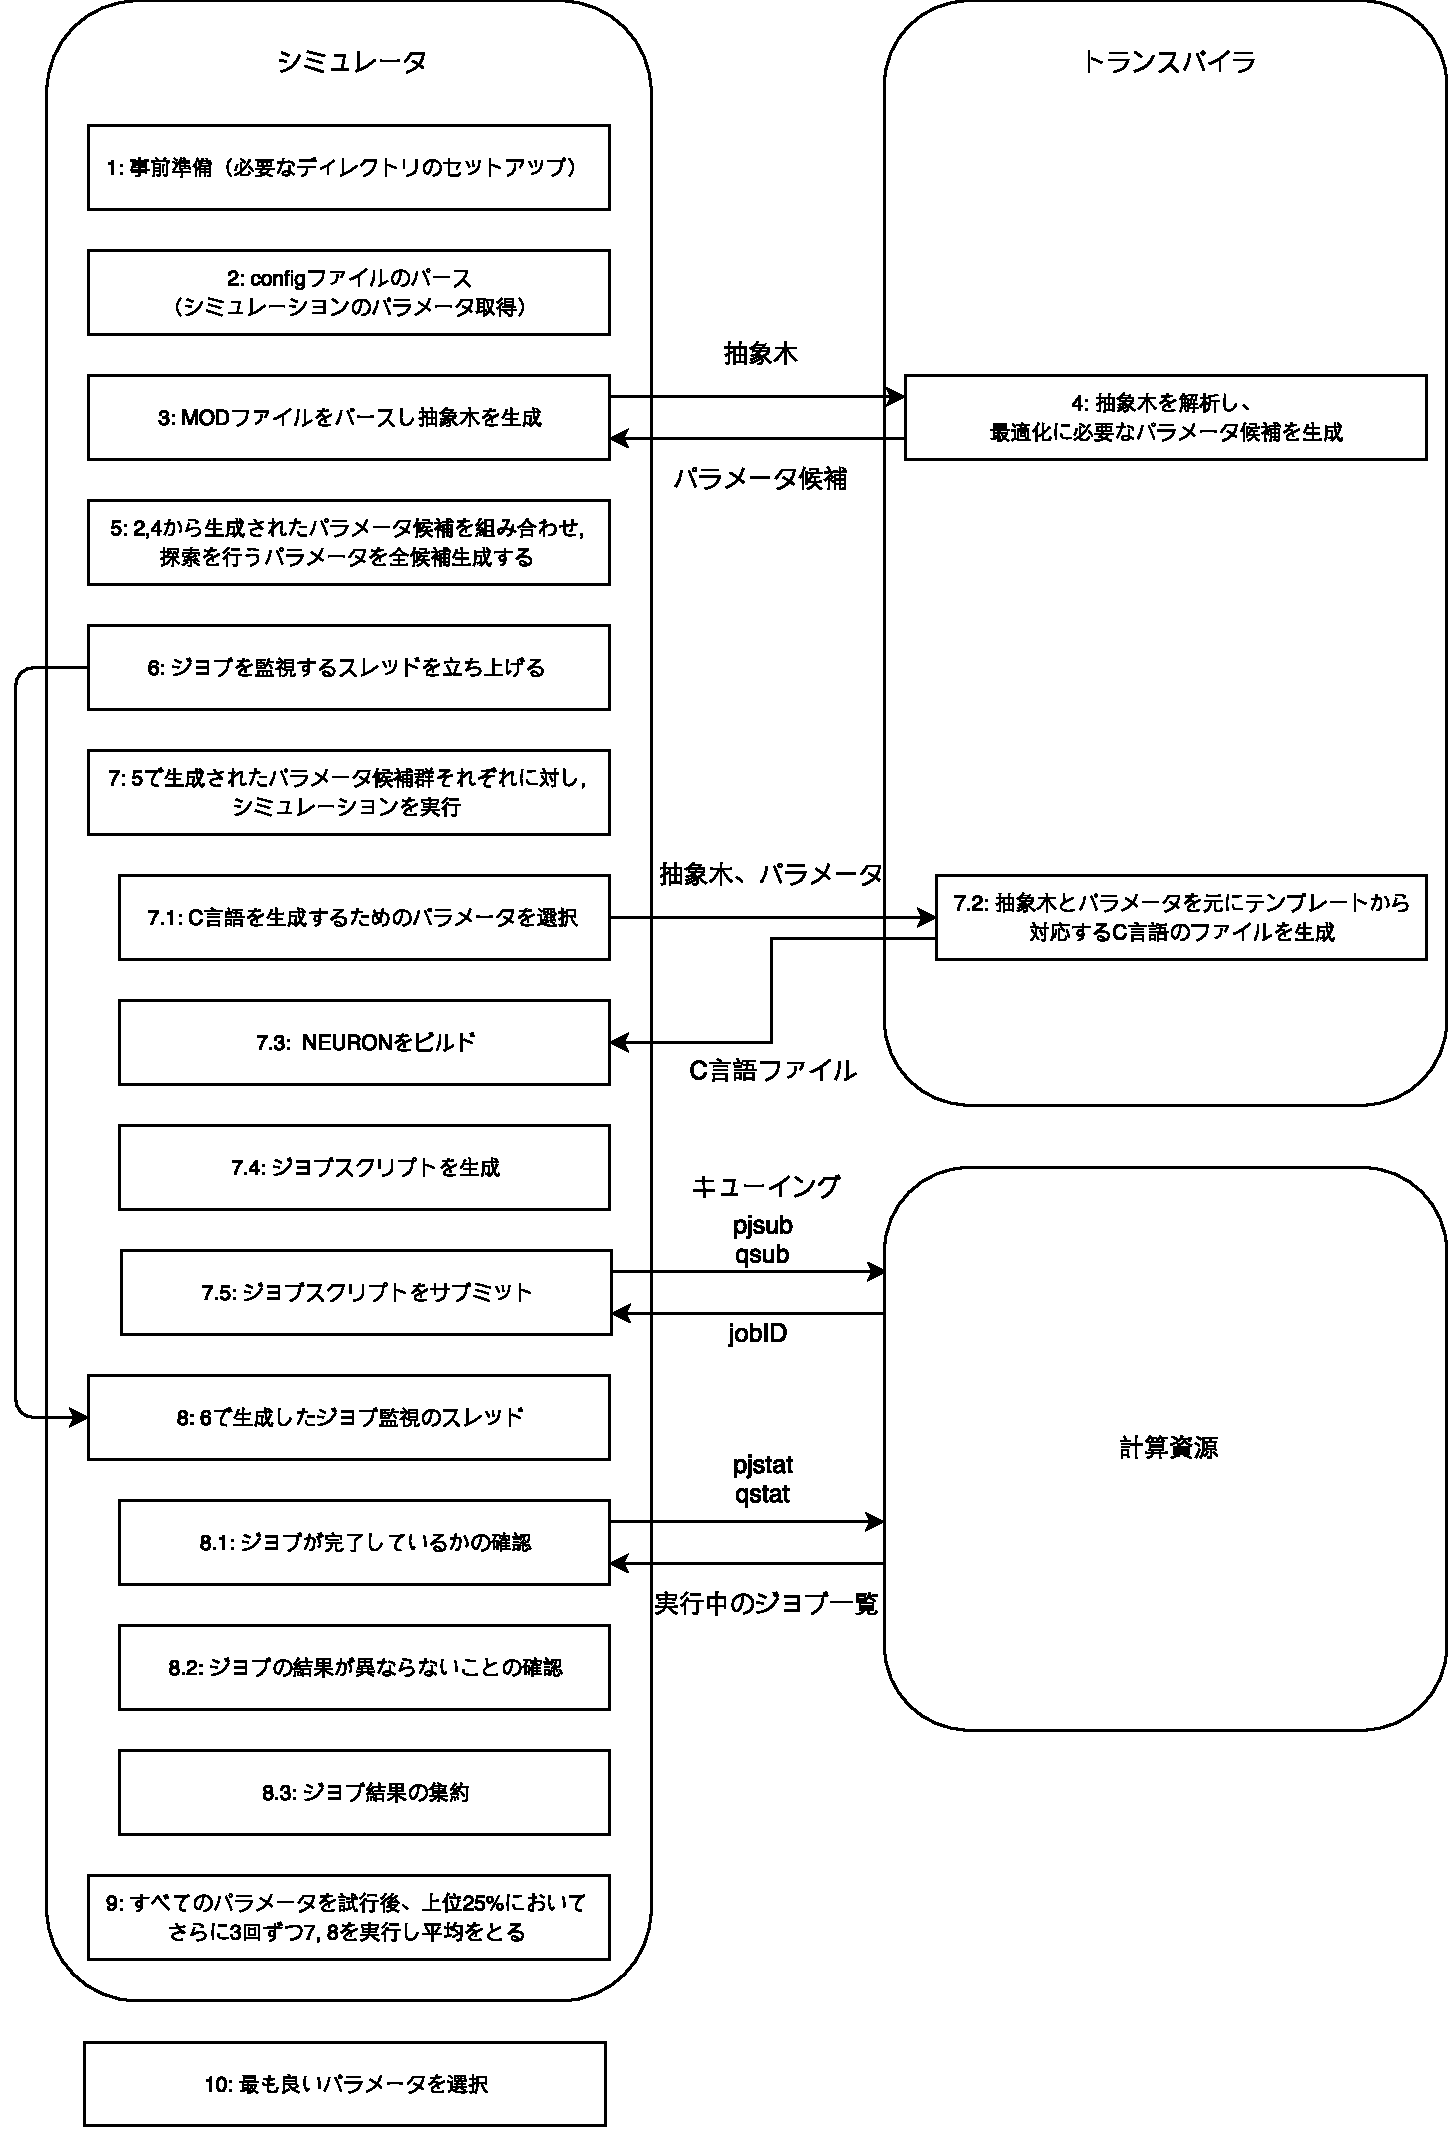
\includegraphics[width=18.0cm]{./images/Genie.pdf}
    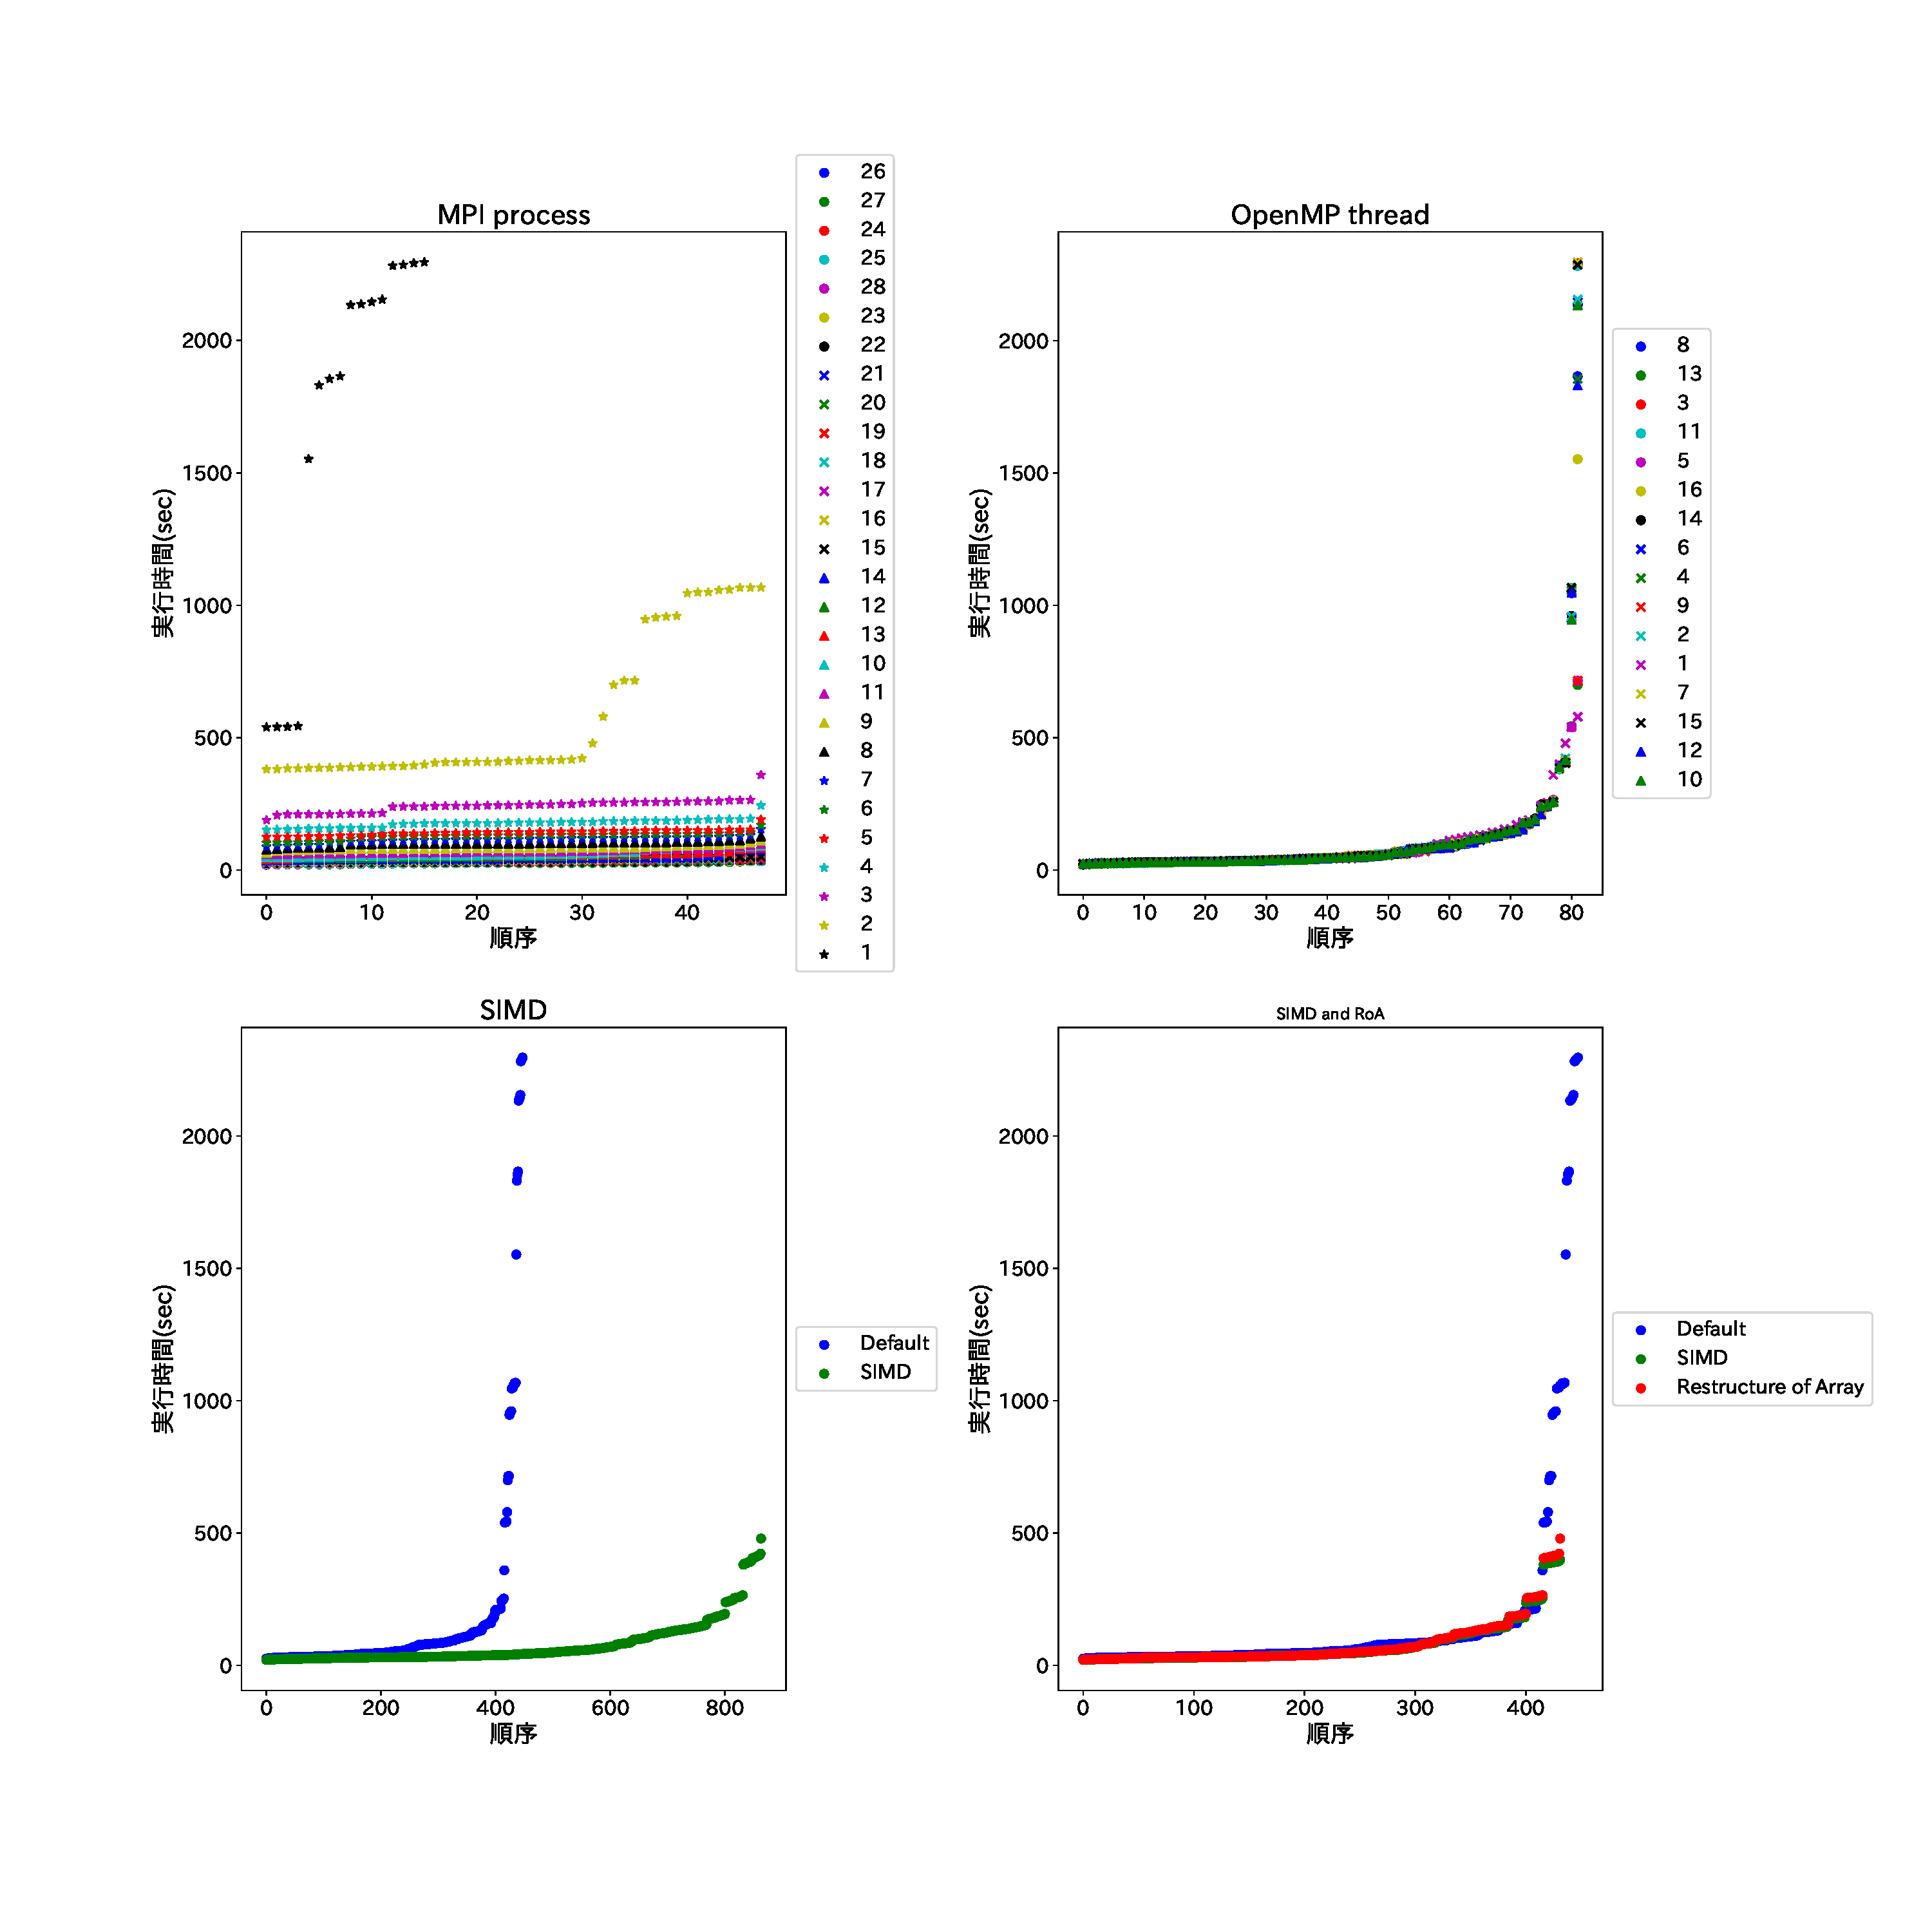
\includegraphics[width=14cm]{./images/cluster-bench.pdf}
    \caption{クラスタ 小規模シミュレーション結果}
    \label{fig:cluster-bench}
 \end{center}
\end{figure}
 一方で, この図では実行時間が短い部分が一部の非常に遅い実行時間に影響されて潰れてしまっている.
そこでパラメータと実行時間の関係を見るために, シミュレータでも利用している実行時間の上位25\%を用いる. その結果を図\ref{fig:cluster-bench-top25}に示す.\\
\begin{figure}[htb]
% h:here, t:top, b:bottom, p:page
 \begin{center}
%    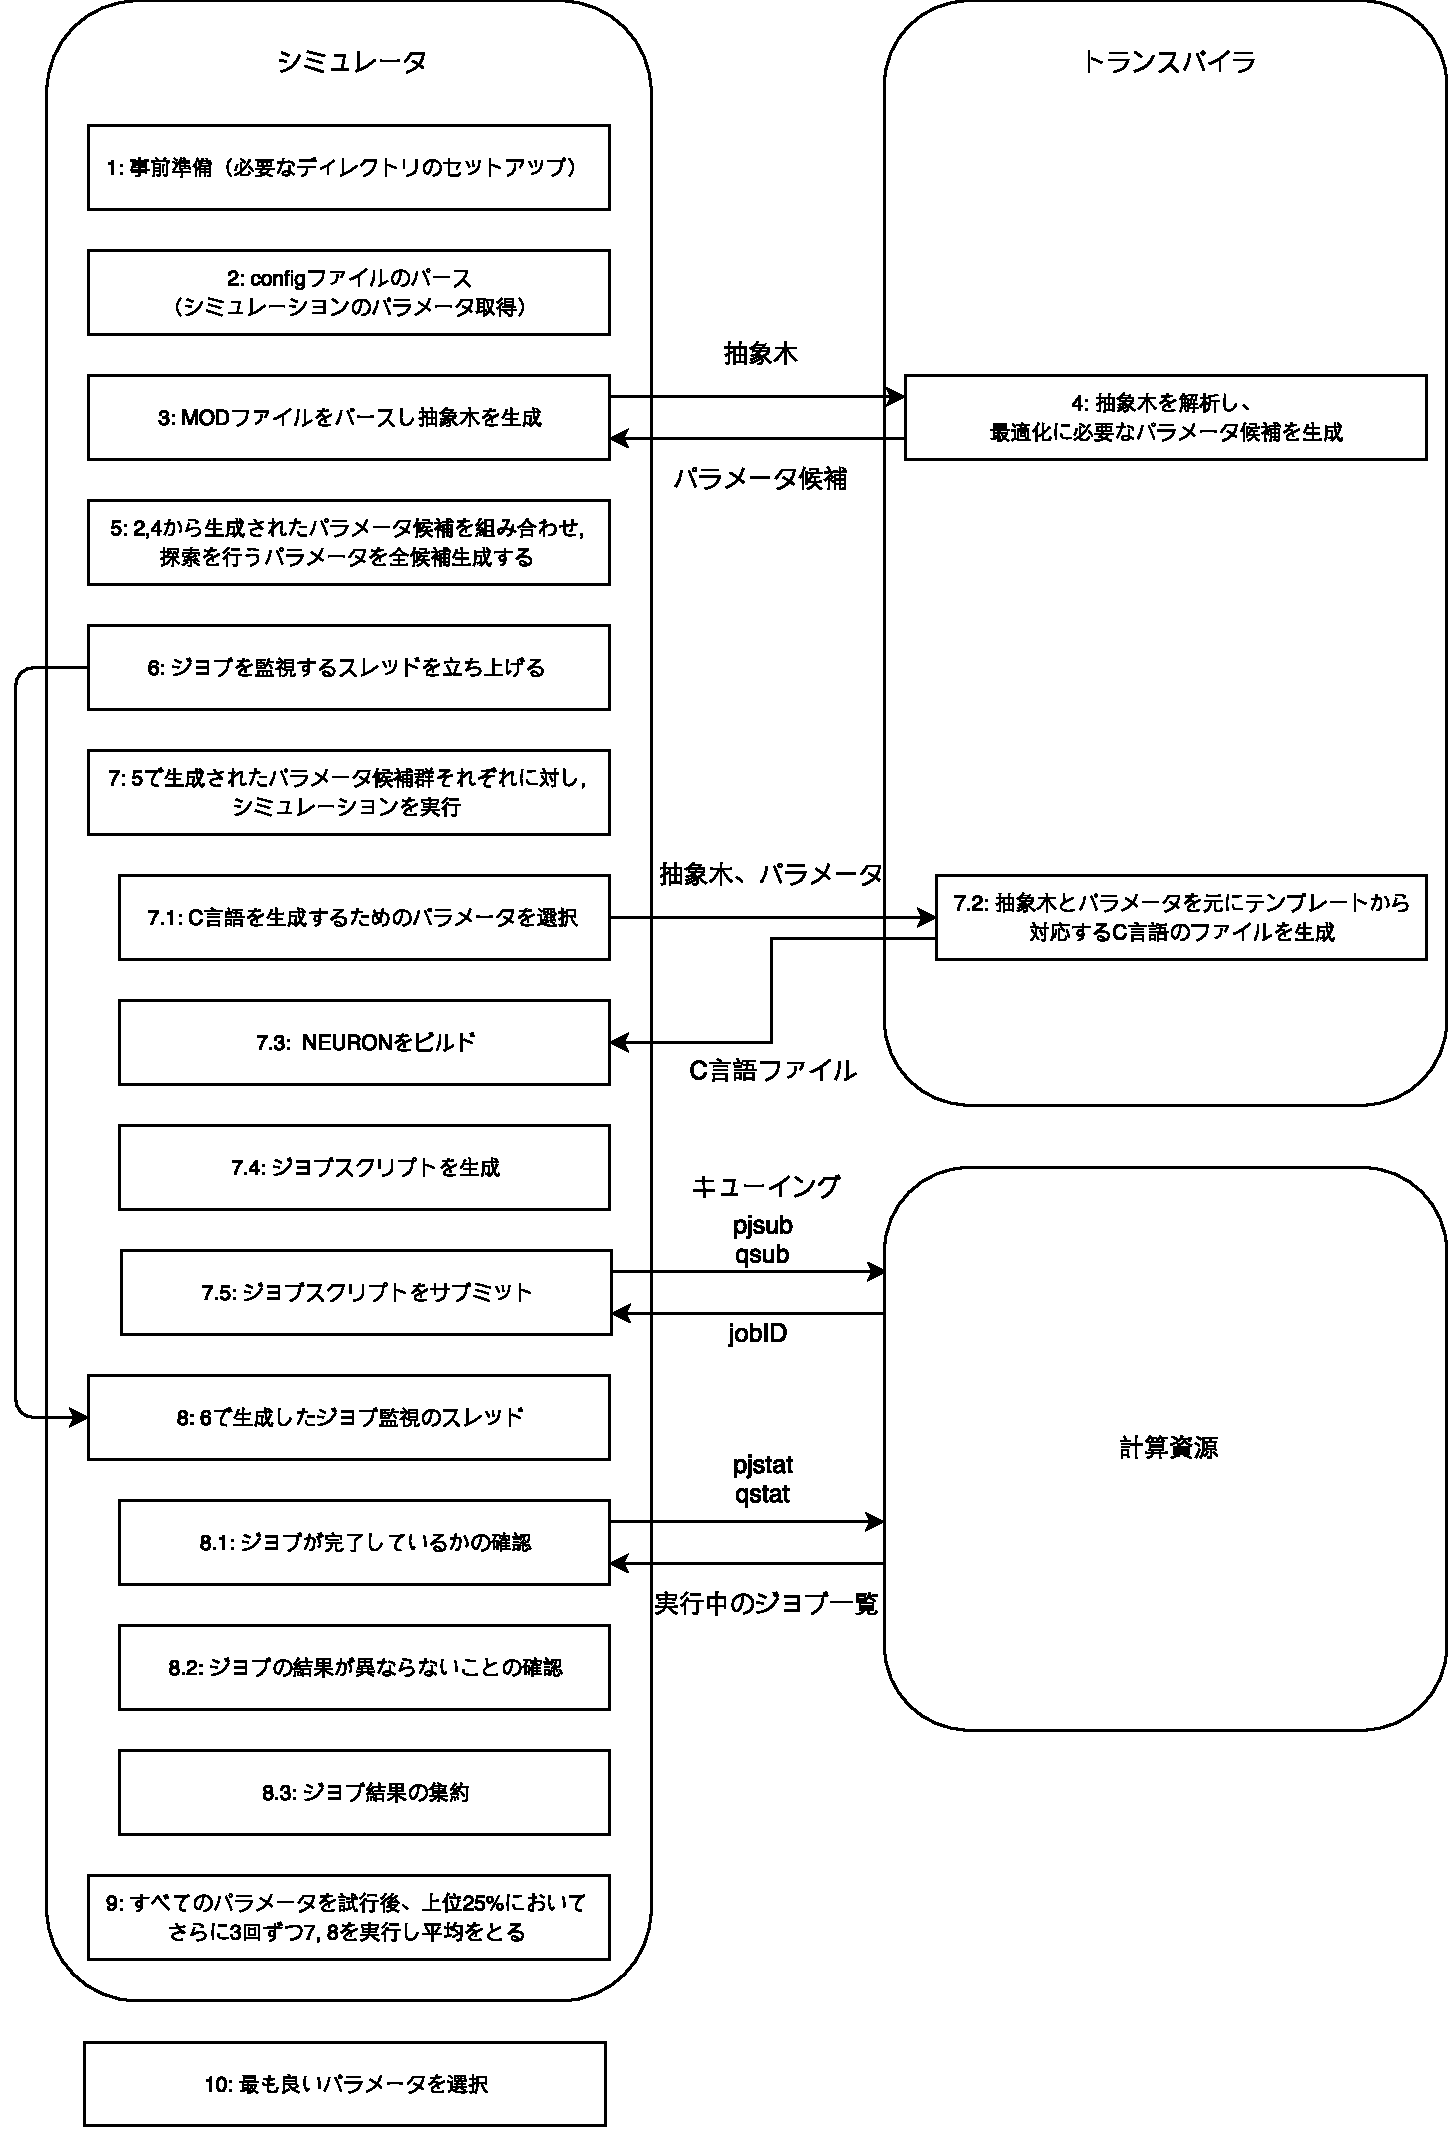
\includegraphics[width=18.0cm]{./images/Genie.pdf}
    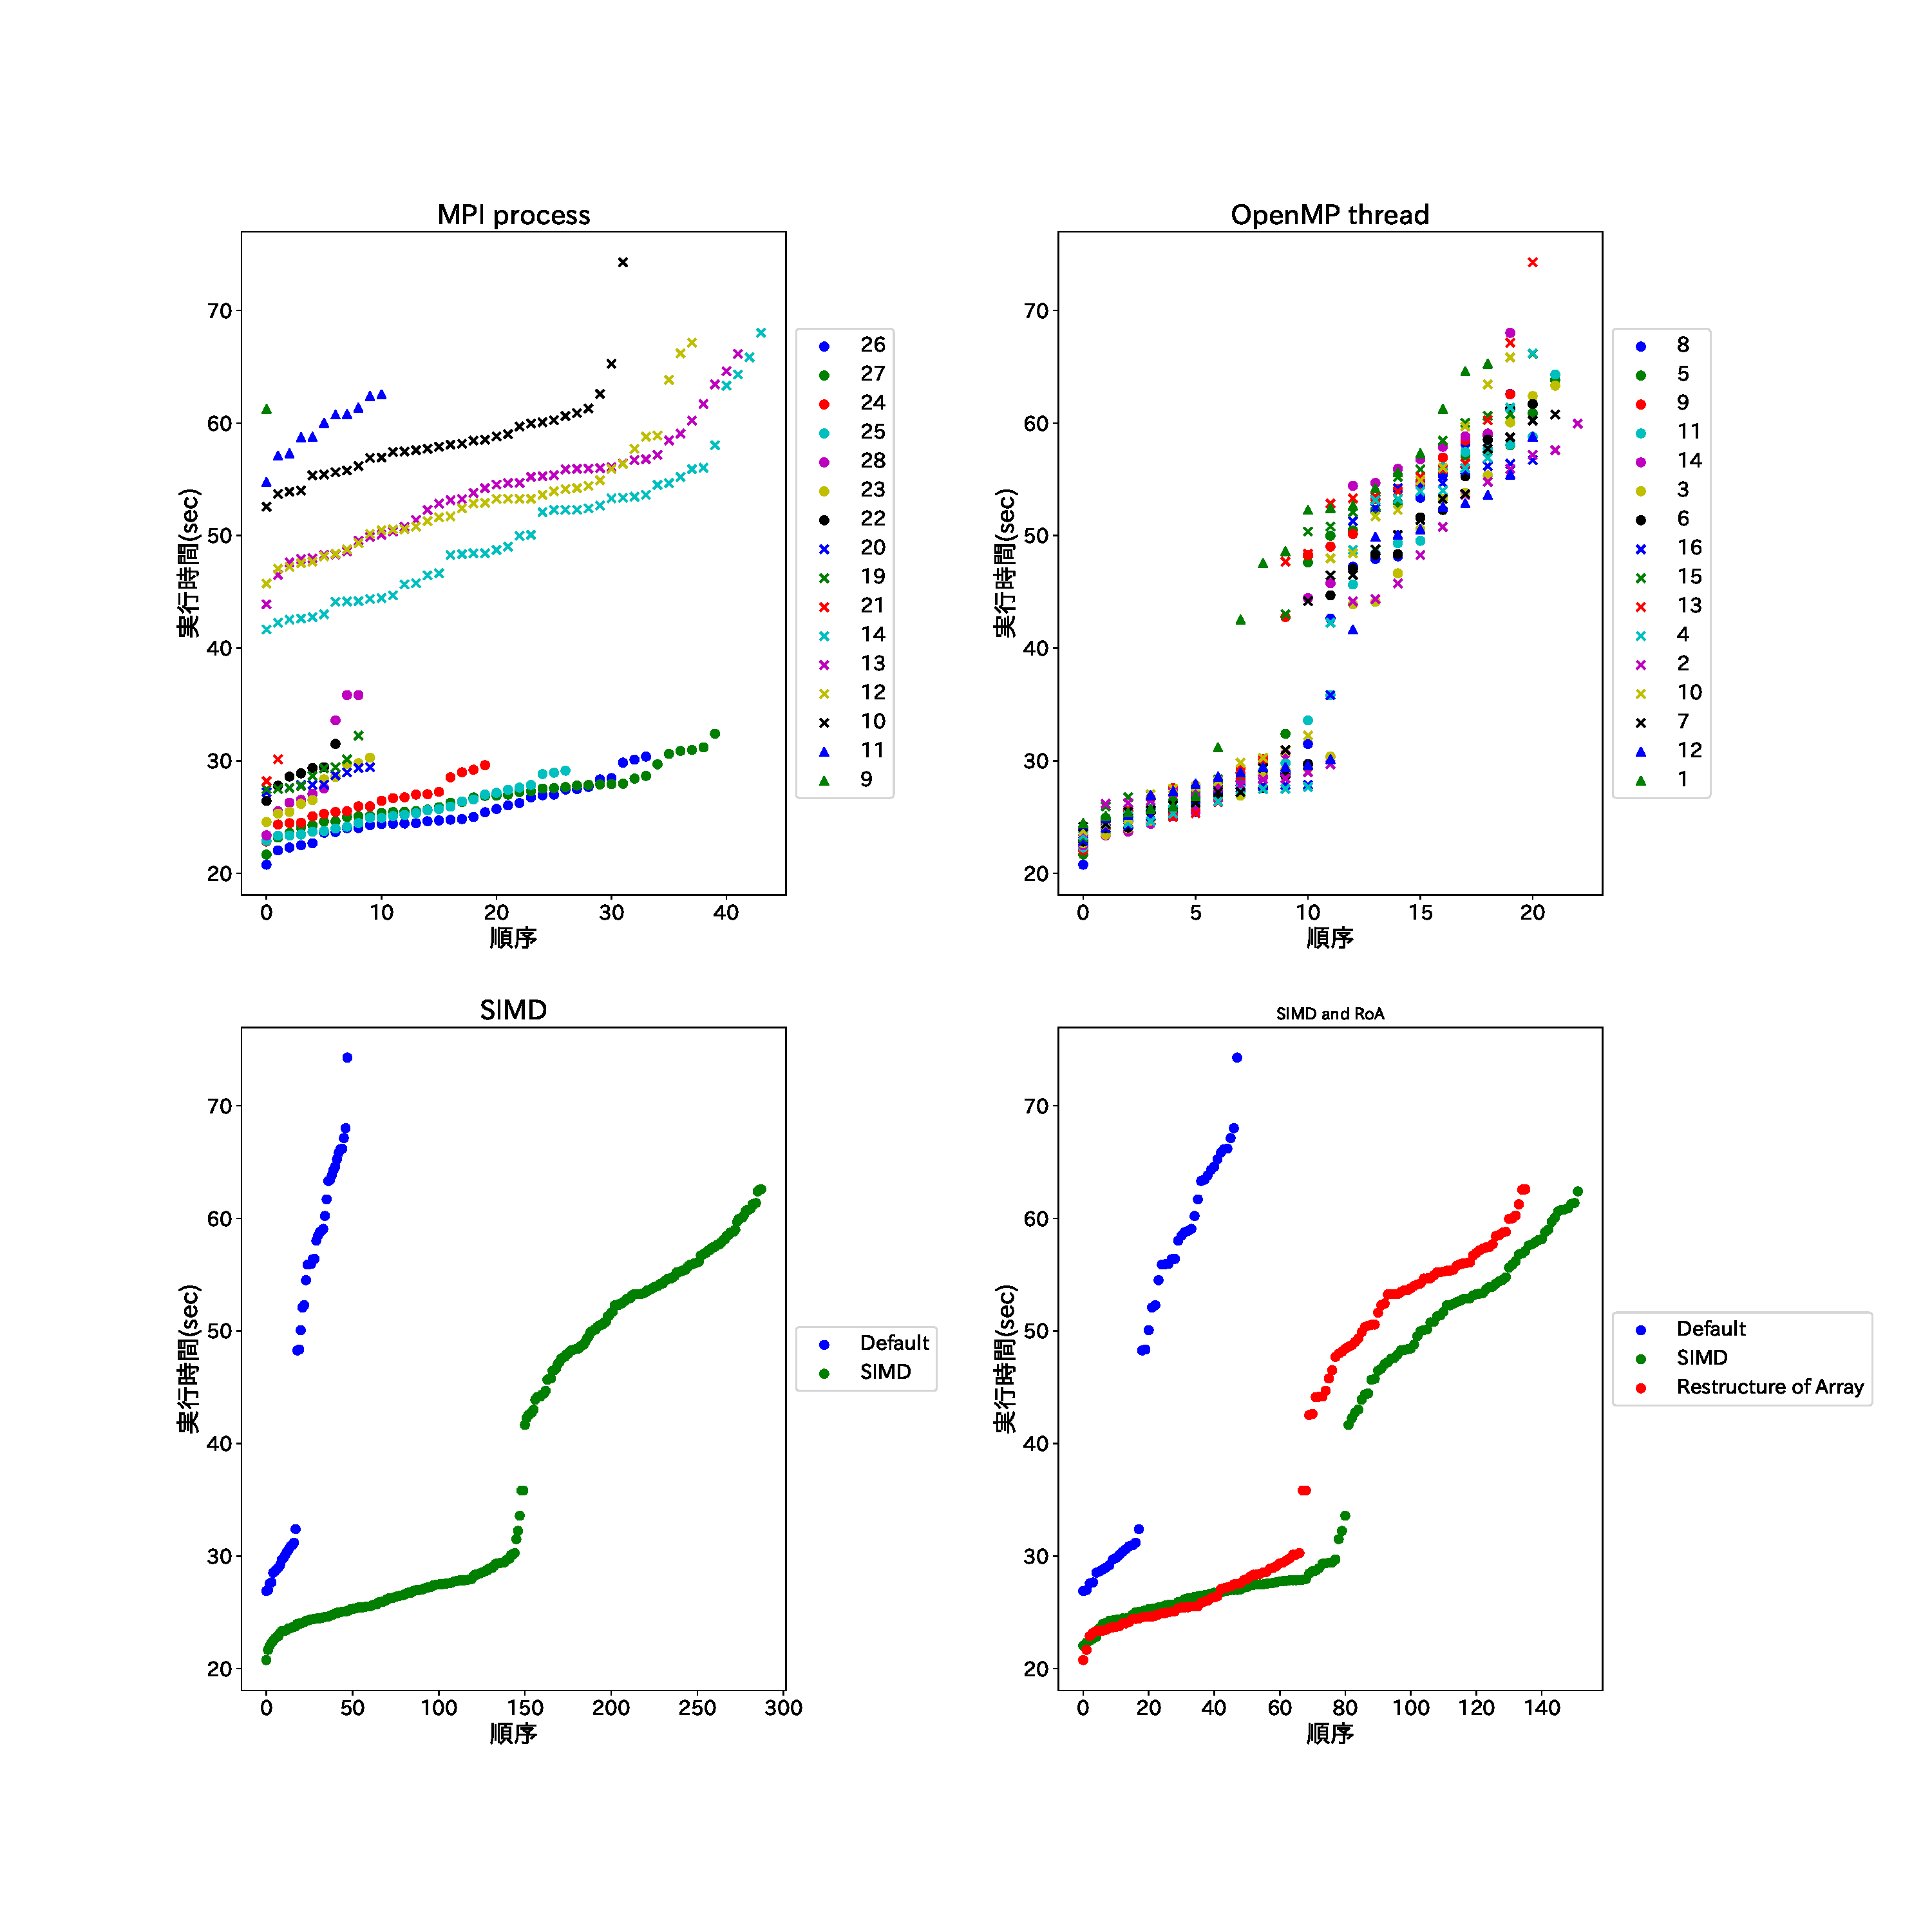
\includegraphics[width=14cm]{./images/cluster-bench-top25.pdf}
    \caption{クラスタ 小規模シミュレーション結果 上位25\%}
    \label{fig:cluster-bench-top25}
 \end{center}
\end{figure}
 図\ref{fig:cluster-bench-top25}では, まずMPIプロセス数に関してプロセス数が14以下のものとそれよりも大きいものの間で実行時間に大きな乖離があることがわかる.
本研究において求めるのは, 実行時間がその環境において最も早くなるパラメータ一組であり,
ここで求めたいものは5.2節以降に詳細にシミュレーションを行う意義のあるパラメータ候補であるため,
ためこのように明確に乖離が見られるパラメータは探索対象から除外することができる.\\
 同様にして, 他の条件を固定した状態でパラメータの除外を行いパラメータによる有意差が生まれなくなるまで絞り込みを行った結果が図\ref{fig:cluster-bench-adjusted-final}である.\\
\begin{figure}[htb]
% h:here, t:top, b:bottom, p:page
\begin{center}
%    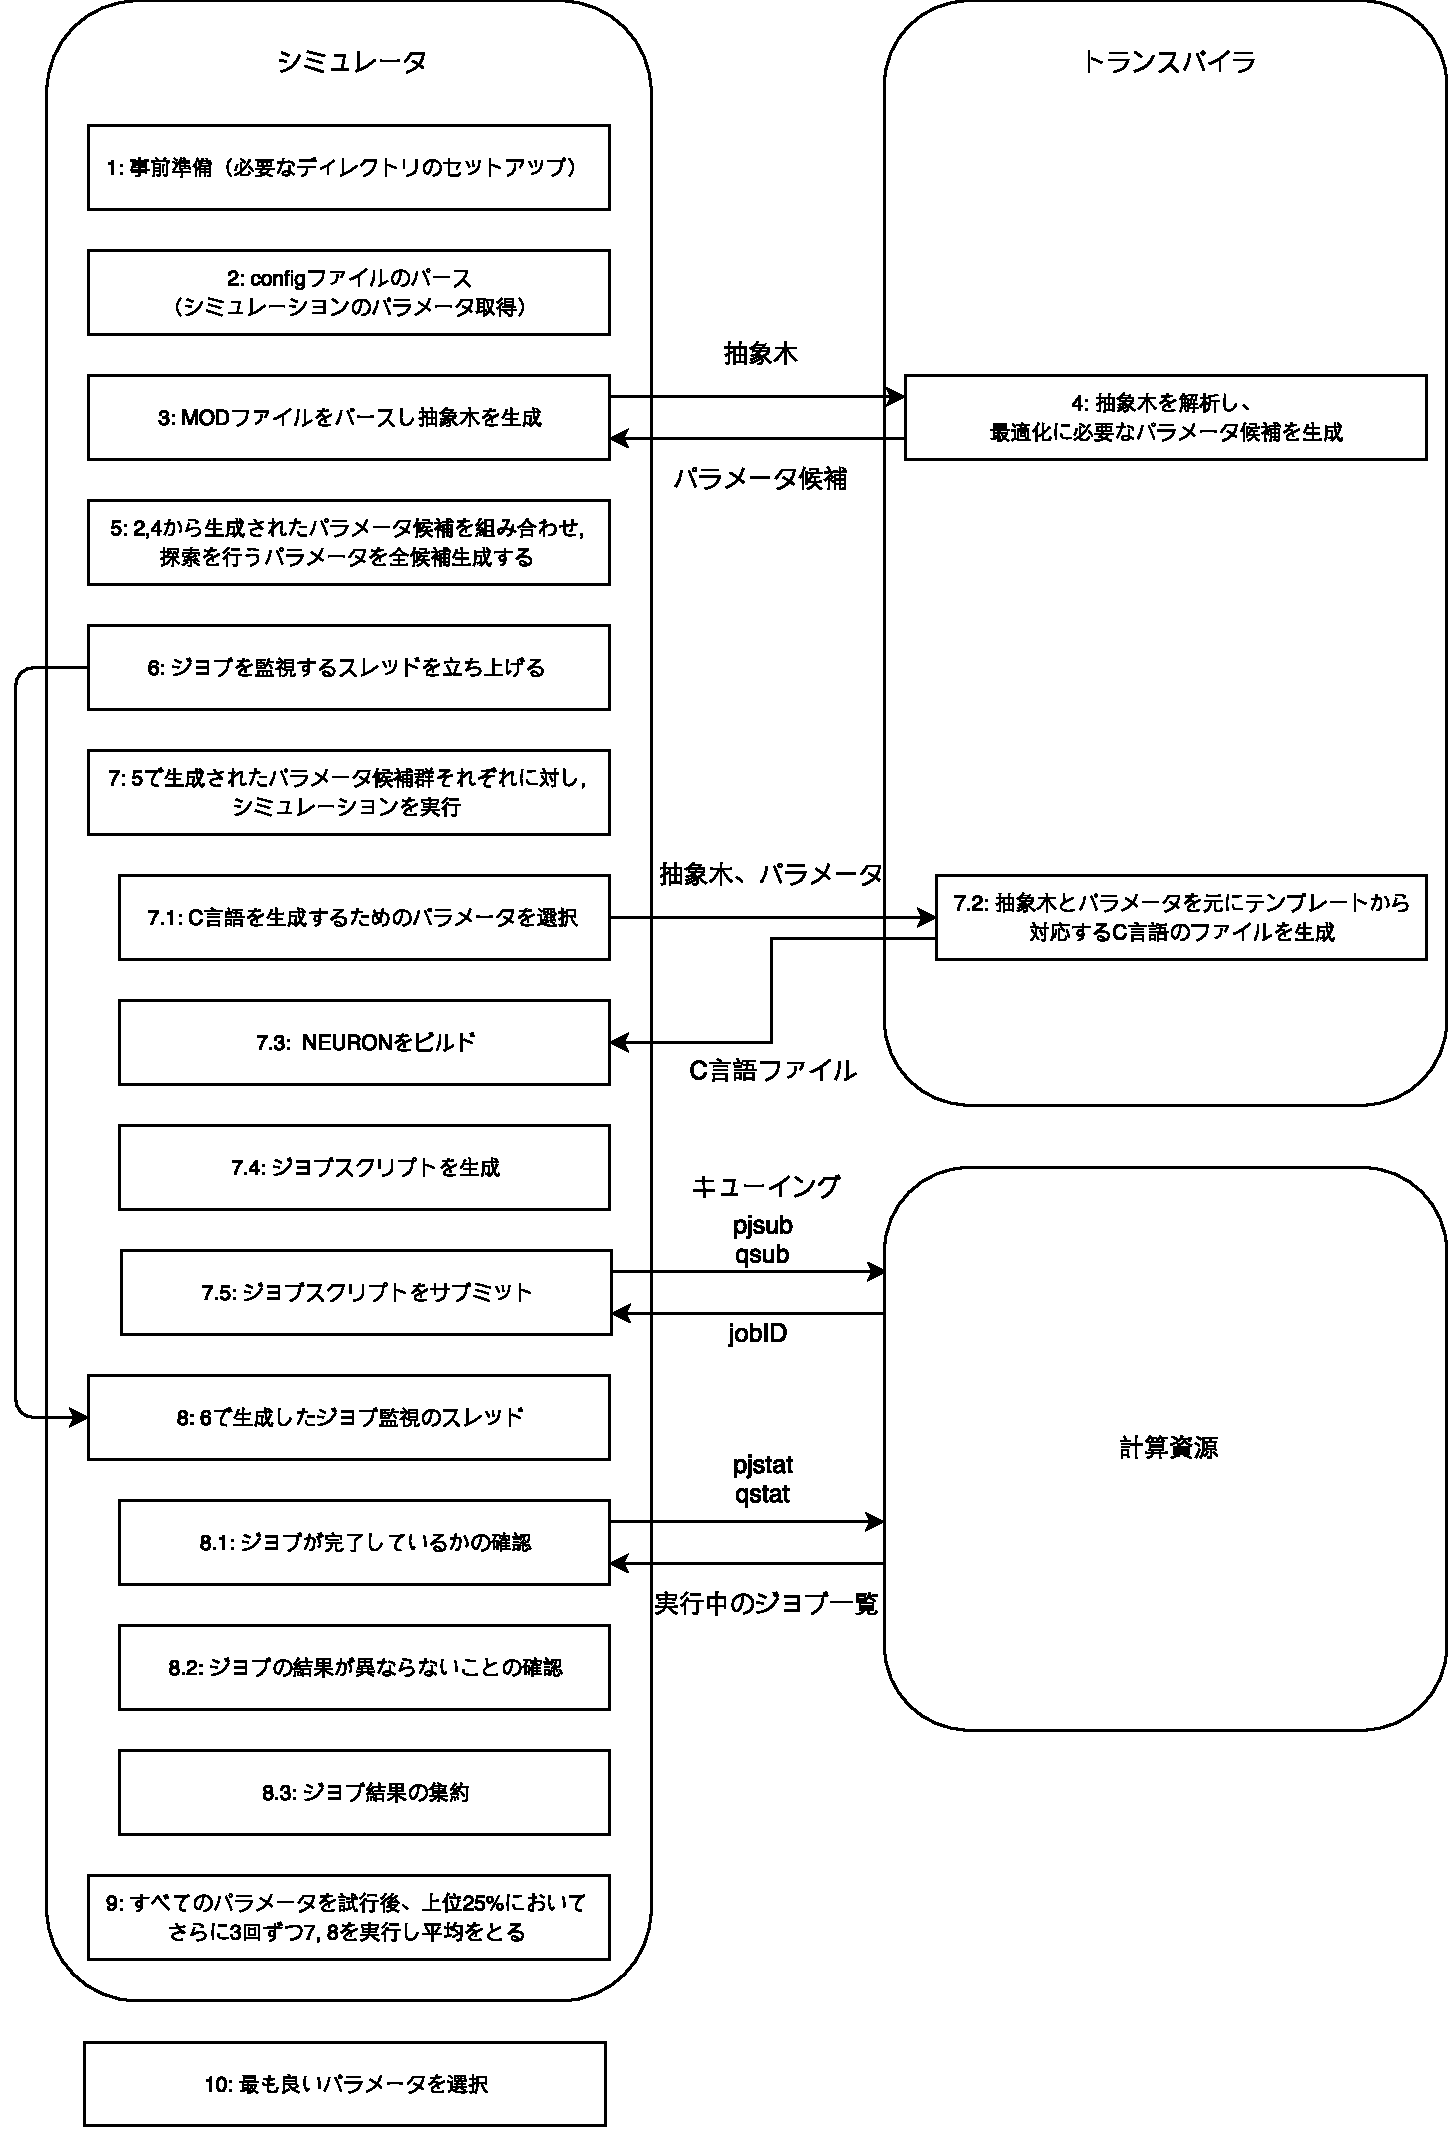
\includegraphics[width=18.0cm]{./images/Genie.pdf}
    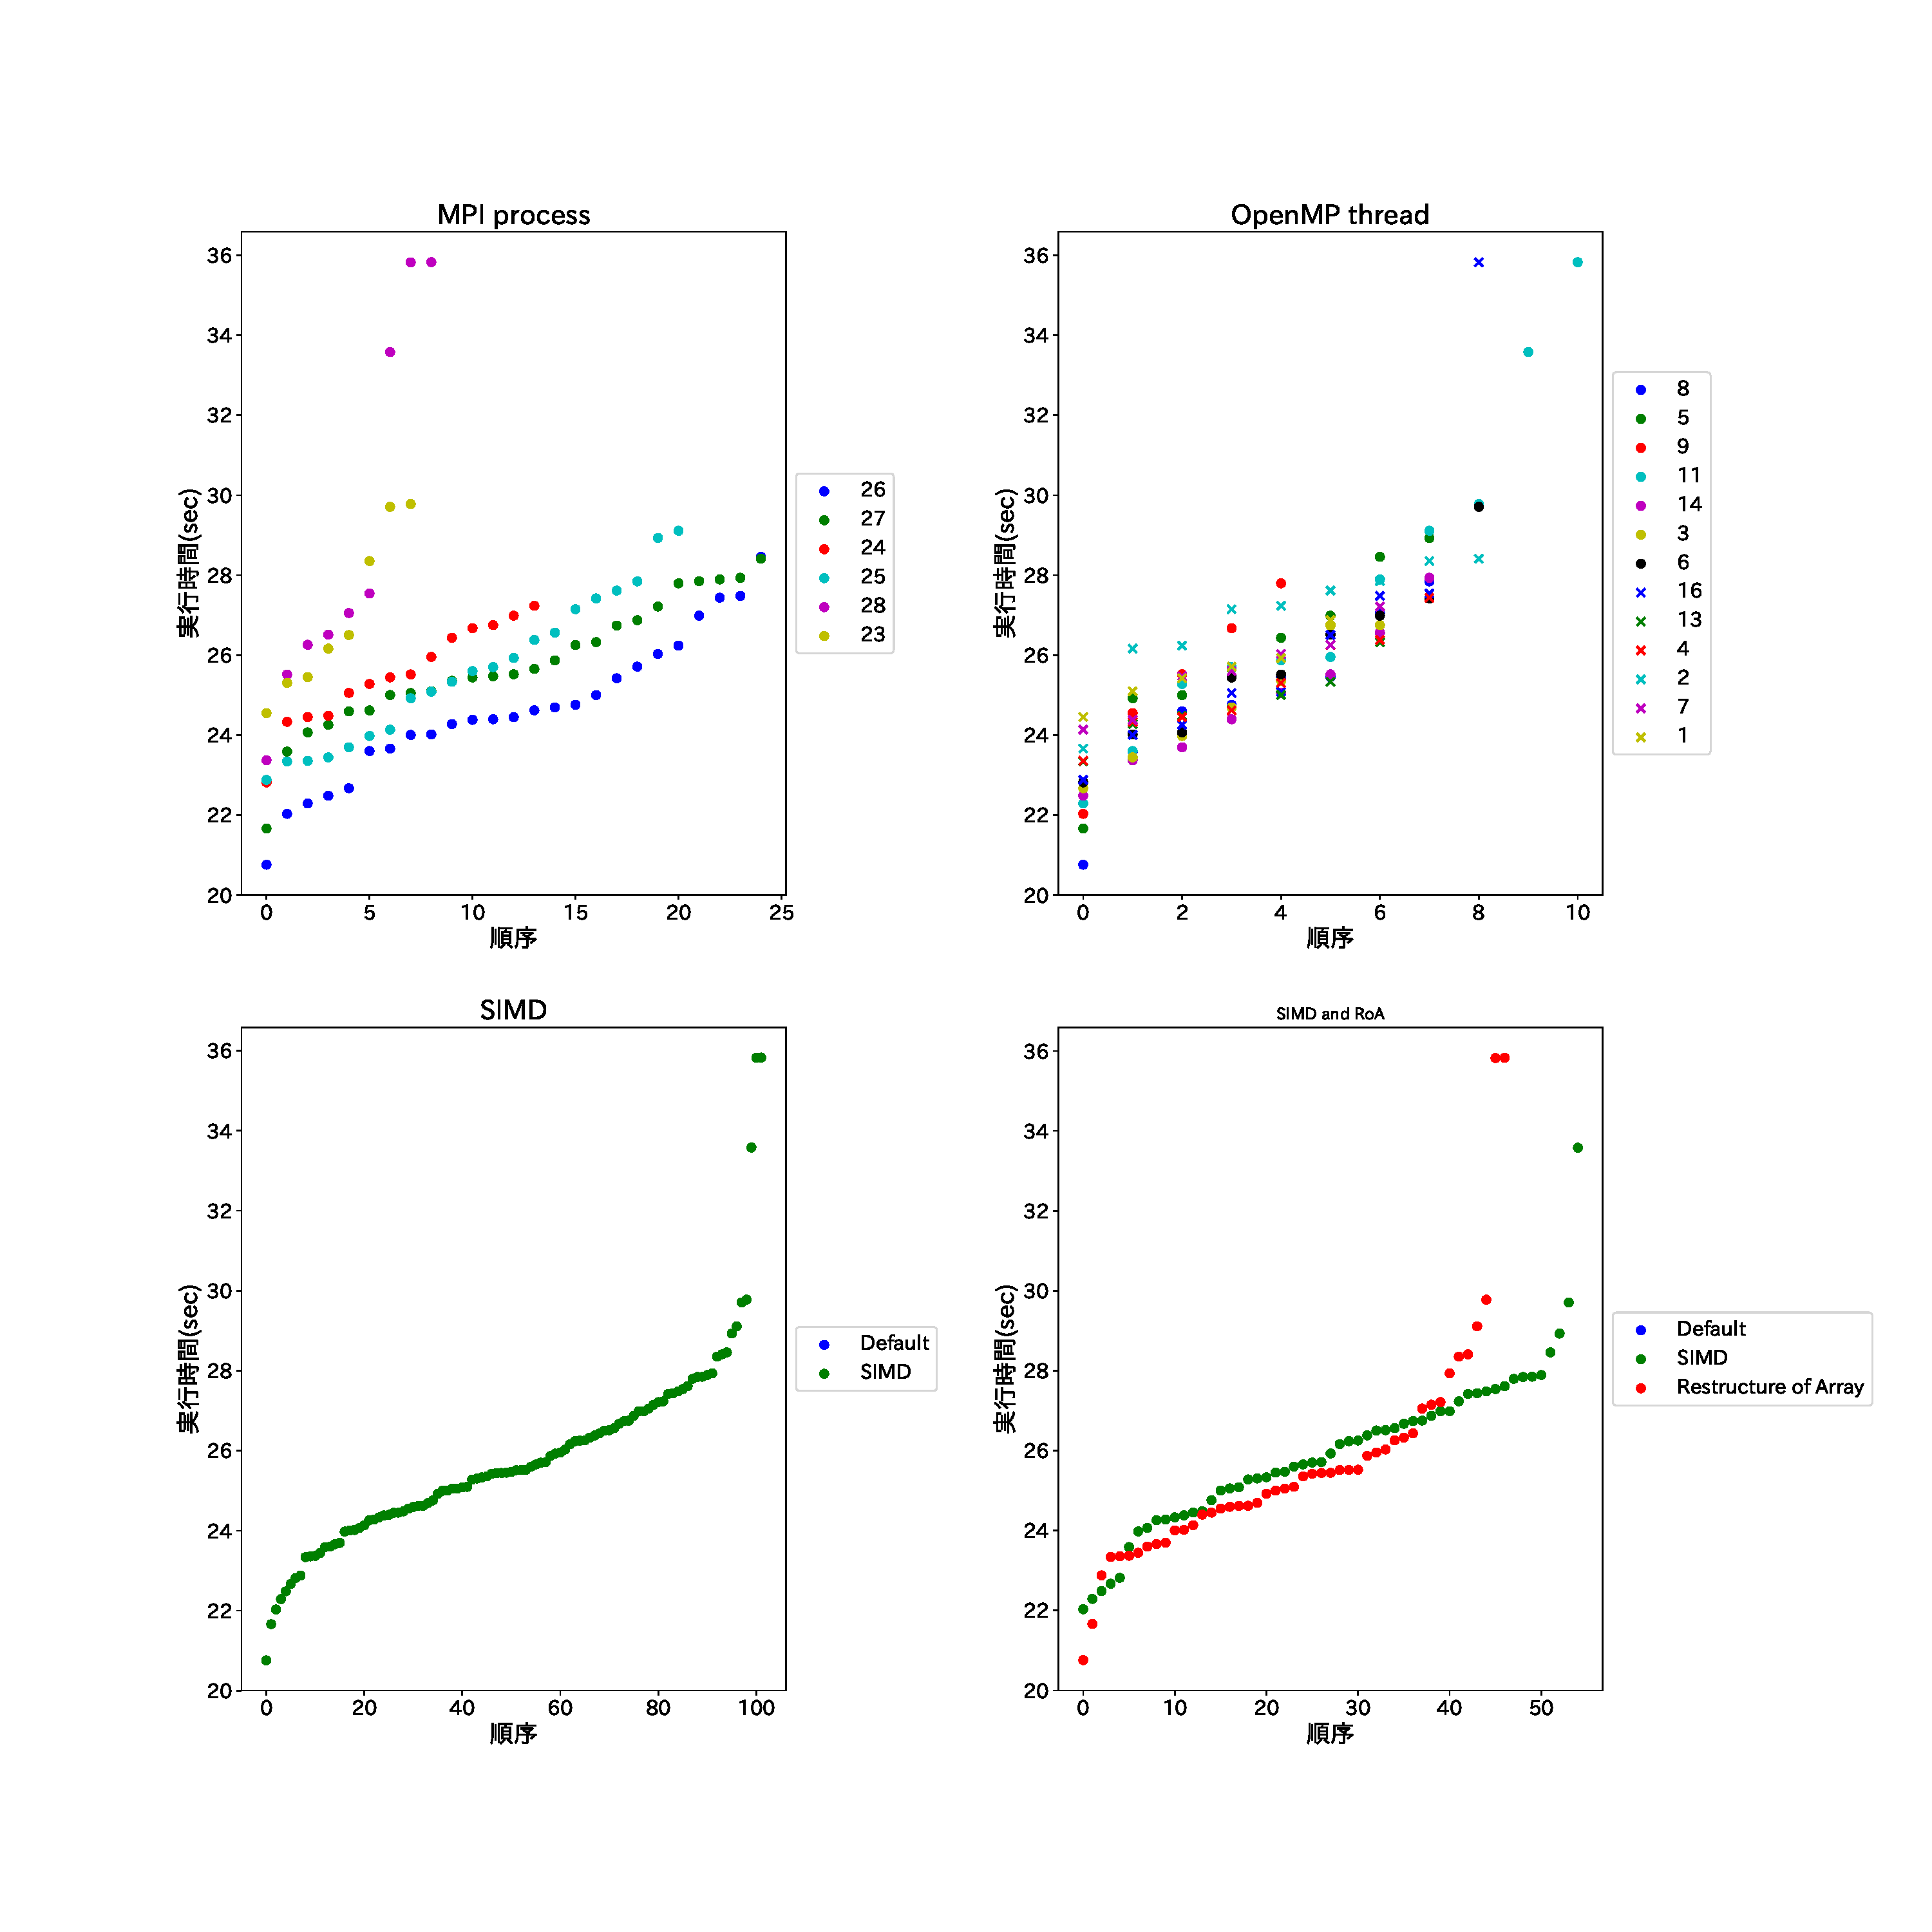
\includegraphics[width=14cm]{./images/cluster-bench-adjusted-final.pdf}
    \caption{クラスタ 小規模シミュレーション結果 パラメータ絞り込み後}
    \label{fig:cluster-bench-adjusted-final}
\end{center}
\end{figure}
\clearpage
 また絞り込みを行った後のパラメータは次のようになる.\\
\begin{table}[htb]
  \caption {クラスタでの絞り込み後のパラメータ}
  \begin{center}
    \begin{tabular}{|p{6cm}|p{8cm}|}
      \hline
      パラメータ & 値の範囲\\ \hline
      ノード数 & 1\\ \hline
      MPIプロセス数 & 23〜28\\ \hline
      OpenMPスレッド数 & [1, 2, 3, 4, 5, 6, 7, 8, 9, 11, 13, 14, 16]\\ \hline
      SIMD化 & 行う\\ \hline
      配列のくくり出し & 行う or 行わない\\ \hline
    \end{tabular}
  \end{center}
\end{table}

\subsubsection{京環境}
\begin{table}[htb]
  \caption {京でのパラメータ}
  \begin{center}
    \begin{tabular}{|p{6cm}|p{8cm}|}
      \hline
      パラメータ & 値の範囲\\ \hline
      ノード数 & 8\\ \hline
      MPIプロセス数 & 1〜8\\ \hline
      OpenMPスレッド数 & 1〜16\\ \hline
      SIMD化 & 行う or 行わない\\ \hline
      配列のくくり出し & 行う(SIMD化を行っているならば) or 行わない\\ \hline
      シミュレーション時間 & 100ms\\ \hline
      神経細胞数 & 256\\ \hline
    \end{tabular}
  \end{center}
\end{table}
 京においてもクラスタ同様パラメータの絞り込みを小規模シミュレーションを用いて行った.\\
 図\ref{fig:k-bench}のMPIプロセス数に着目すると, それぞれのプロセス数に対し30番目前後で大きな
隔たりがあることがわかる. SIMDのグラフにおいてもSIMDがデフォルトのソースコードを大きく上回っていること,
またシミュレーションの設定上SIMDとそうでないものが2対1の比率であり,
30番目付近を境としたMPIプロセス数における比率と同じであることからこの隔たりはSIMD化が影響していることがわかる.\\
\begin{figure}[htb]
% h:here, t:top, b:bottom, p:page
\begin{center}
%    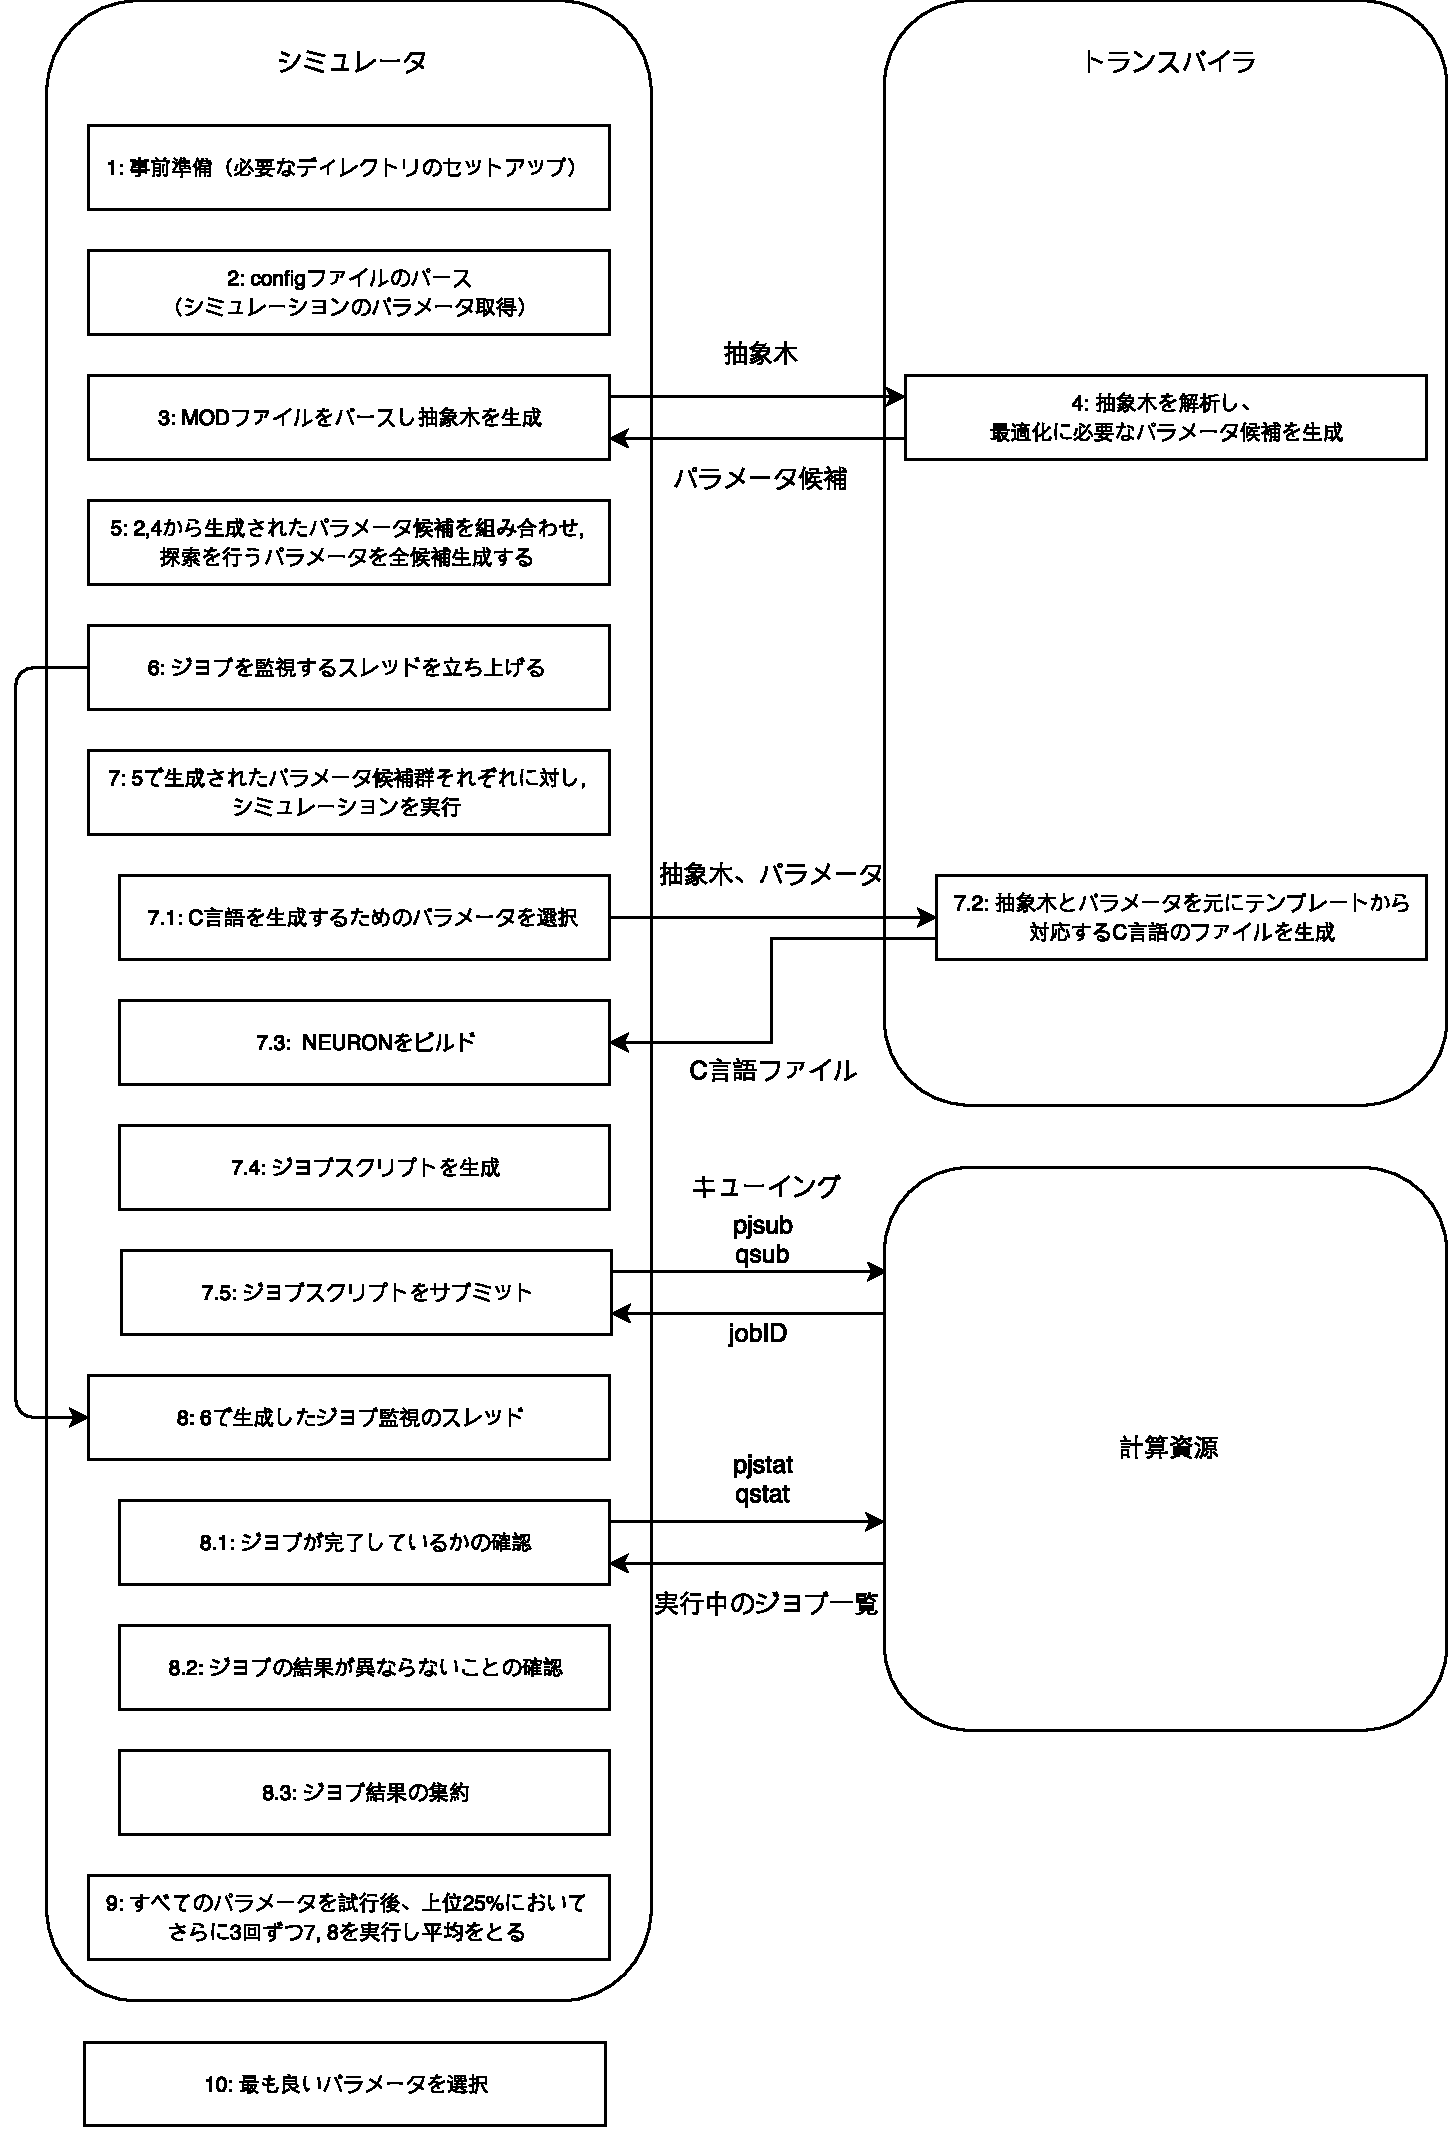
\includegraphics[width=18.0cm]{./images/Genie.pdf}
    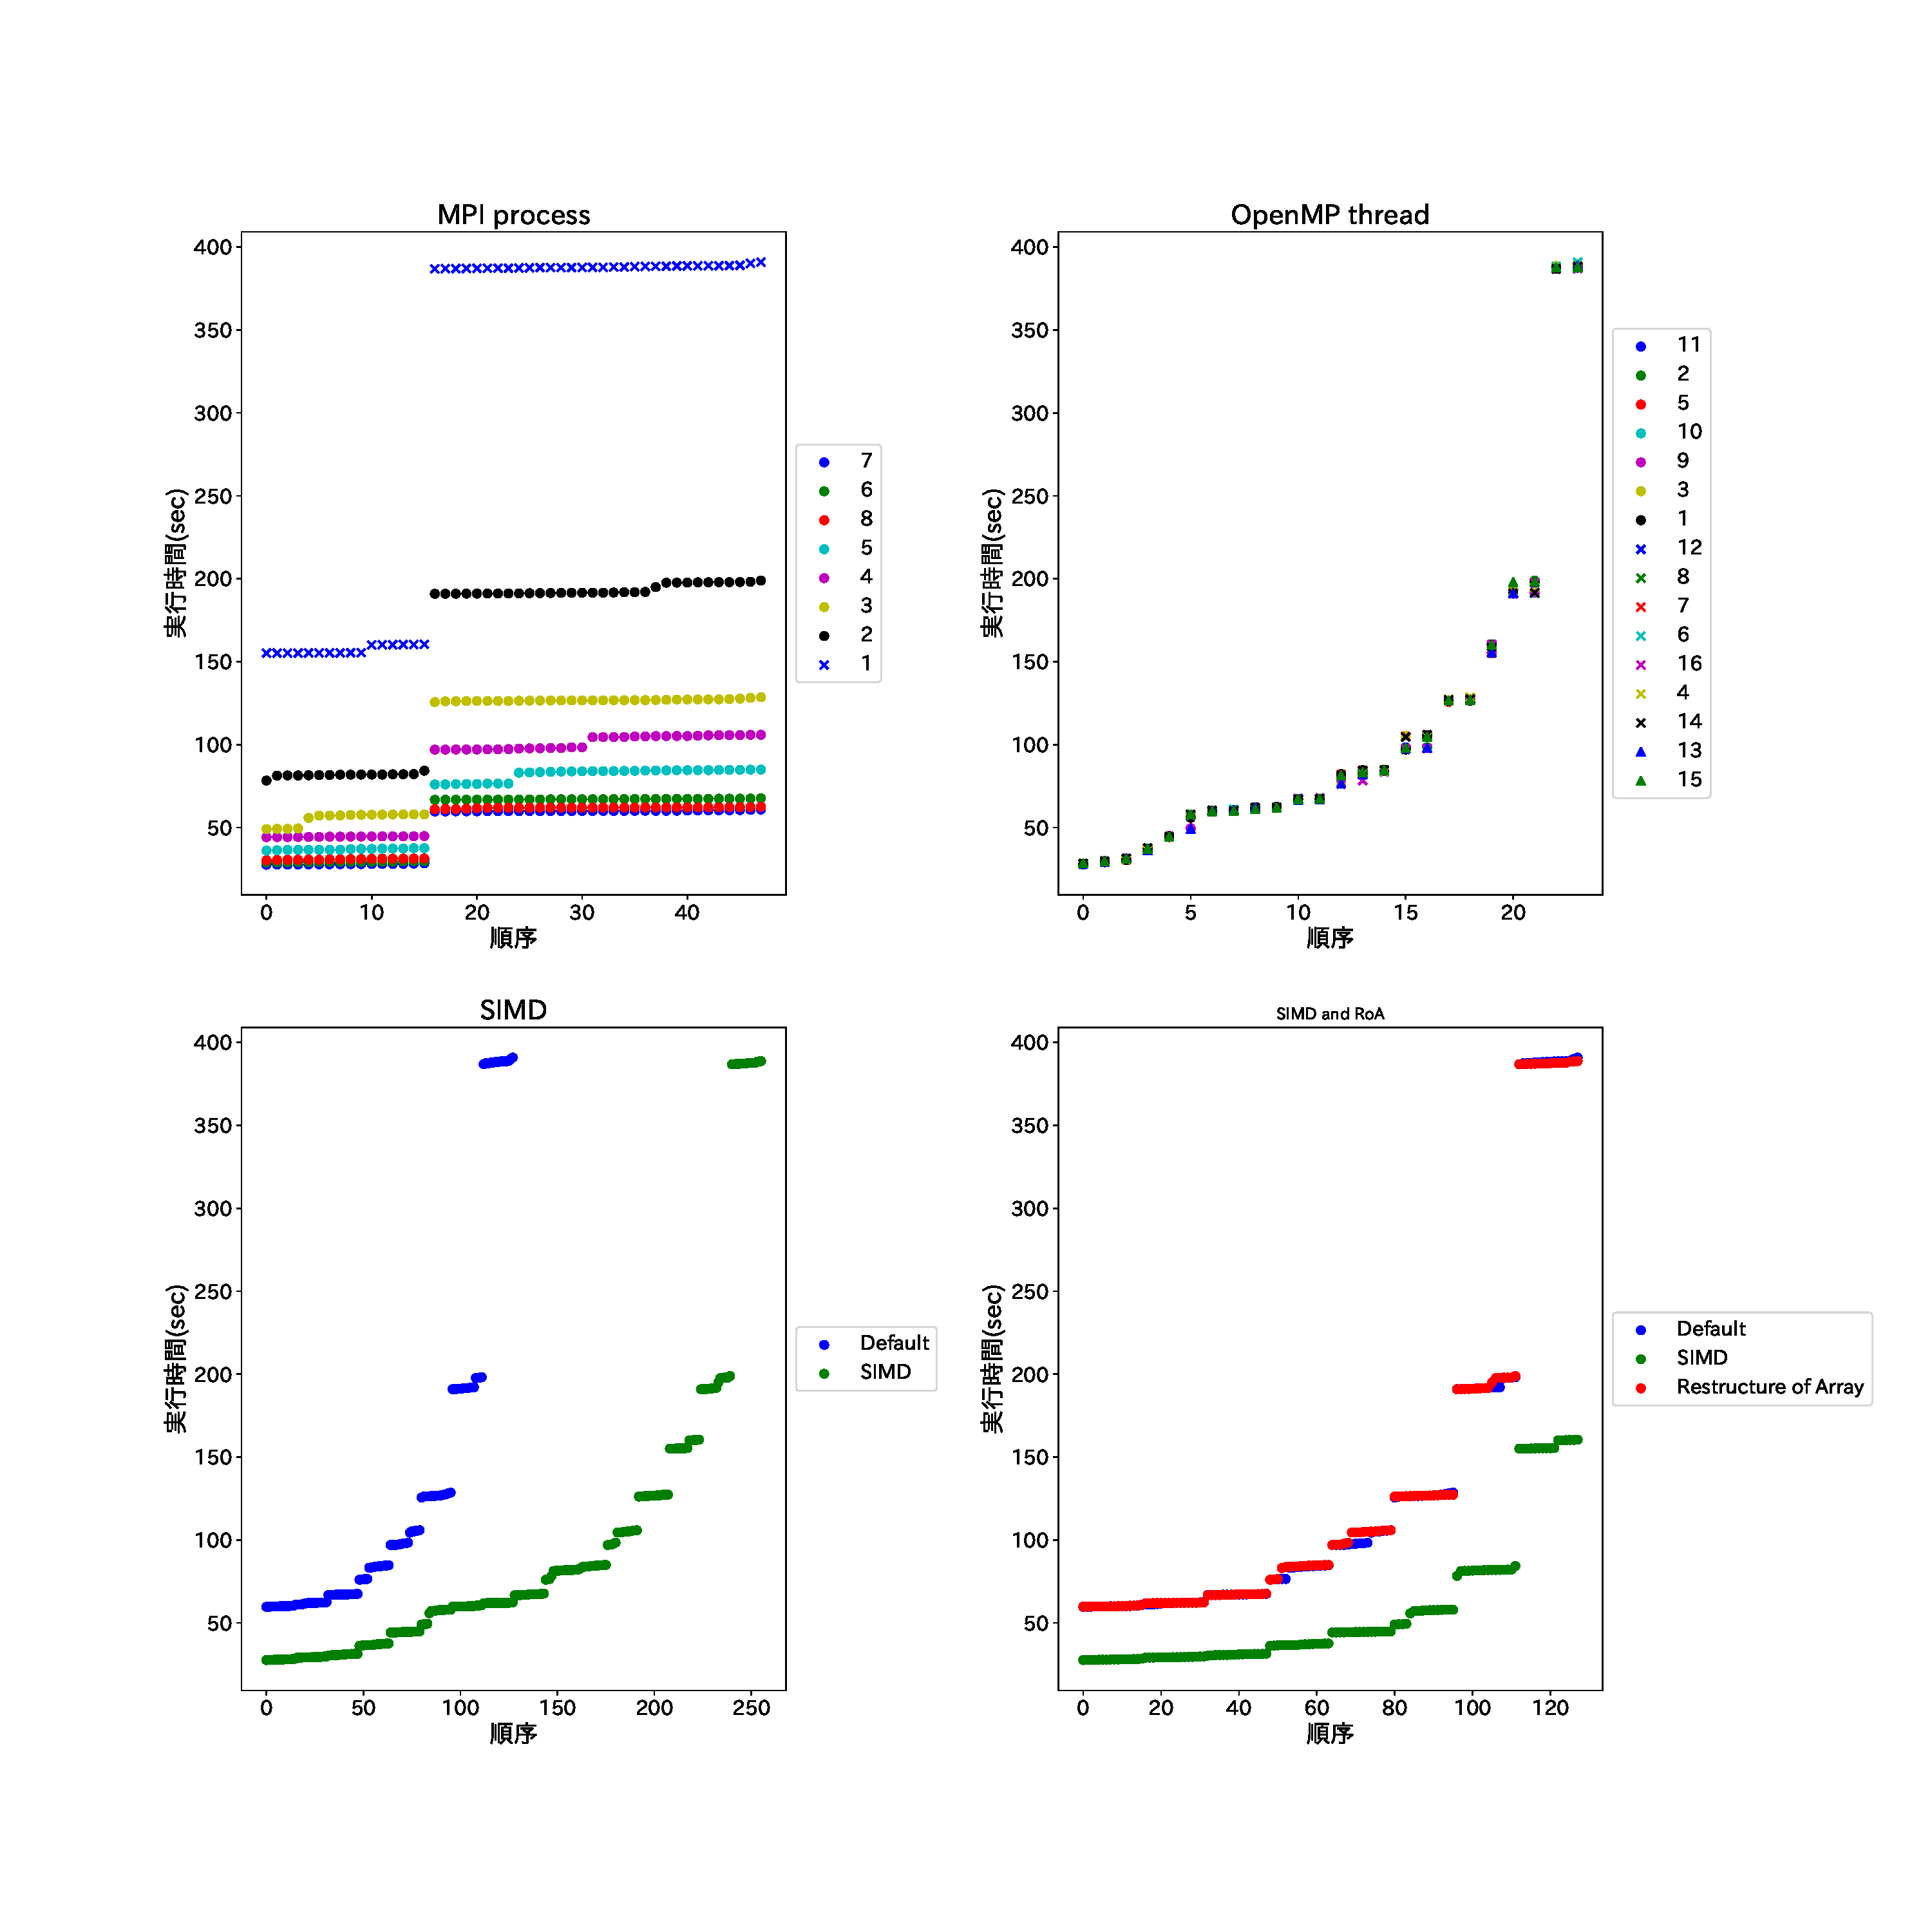
\includegraphics[width=14cm]{./images/k-bench.pdf}
    \caption{京 小規模シミュレーション結果}
    \label{fig:k-bench}
\end{center}
\end{figure}
\clearpage
一方で, シミュレーション結果の実行時間が早い上位25\%のパラメータを示した図\ref{fig:k-bench-top25}では,
プロセス数8のものが他のプロセス数と比較して抜きん出て高速であることが読み取れる.
また, SIMD化されていないパラメータ候補はすでに除外されており,
候補数がすでに十分制限されているためプロセス数とSIMD化のみを絞り込みの条件として用いた.\\

\begin{figure}[htb]
% h:here, t:top, b:bottom, p:page
\begin{center}
%    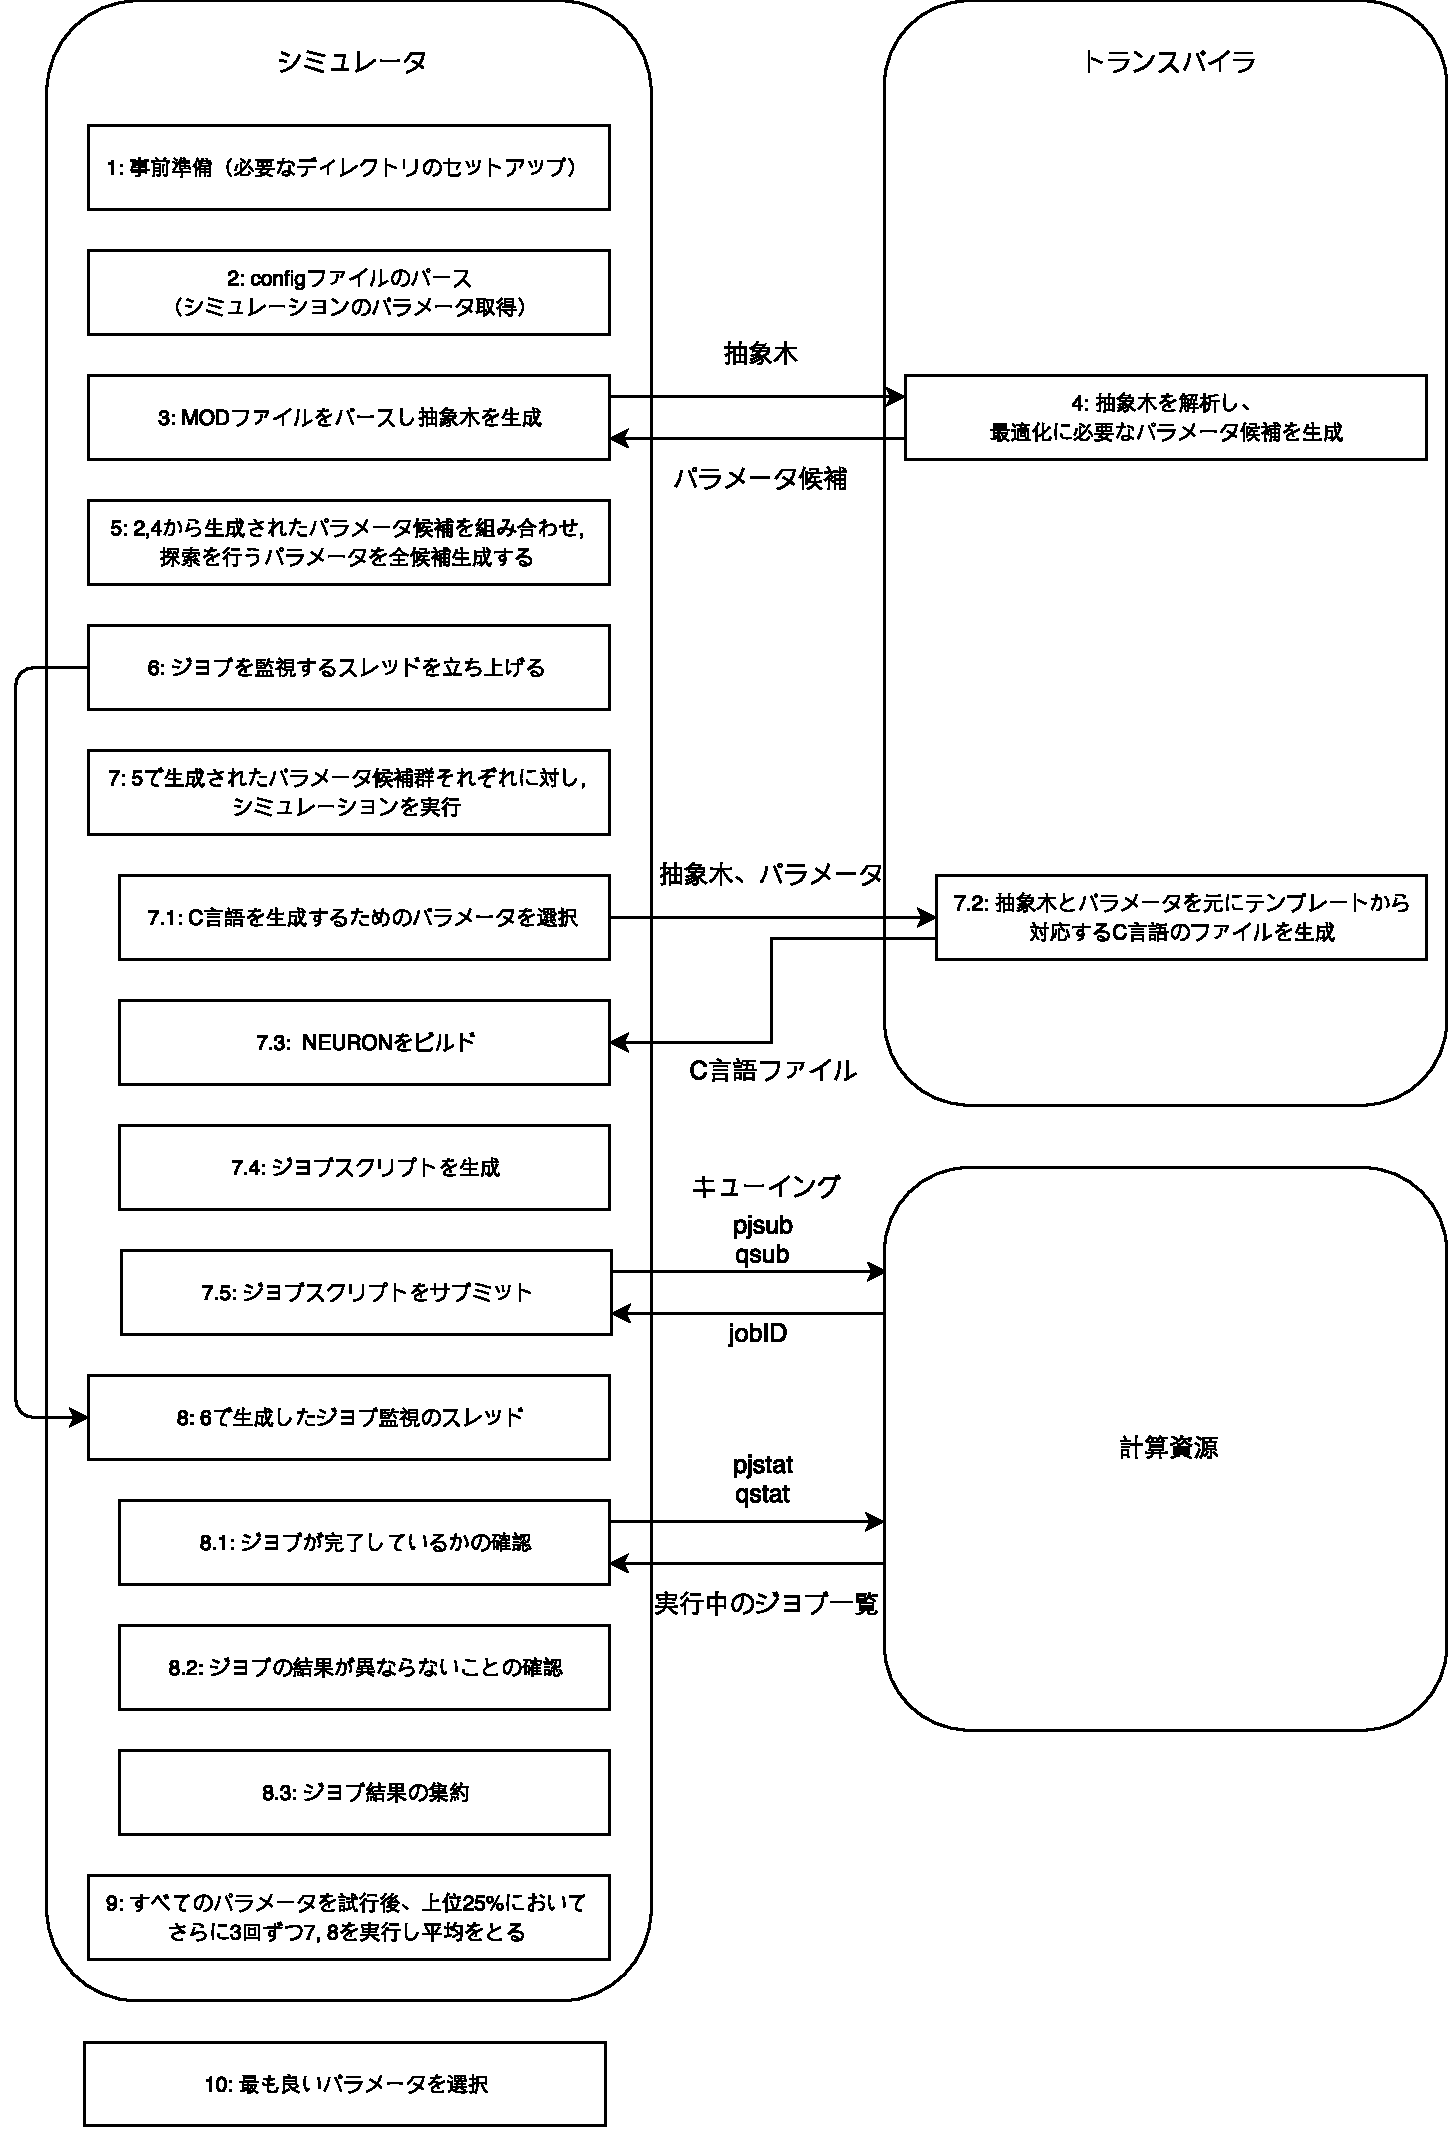
\includegraphics[width=18.0cm]{./images/Genie.pdf}
    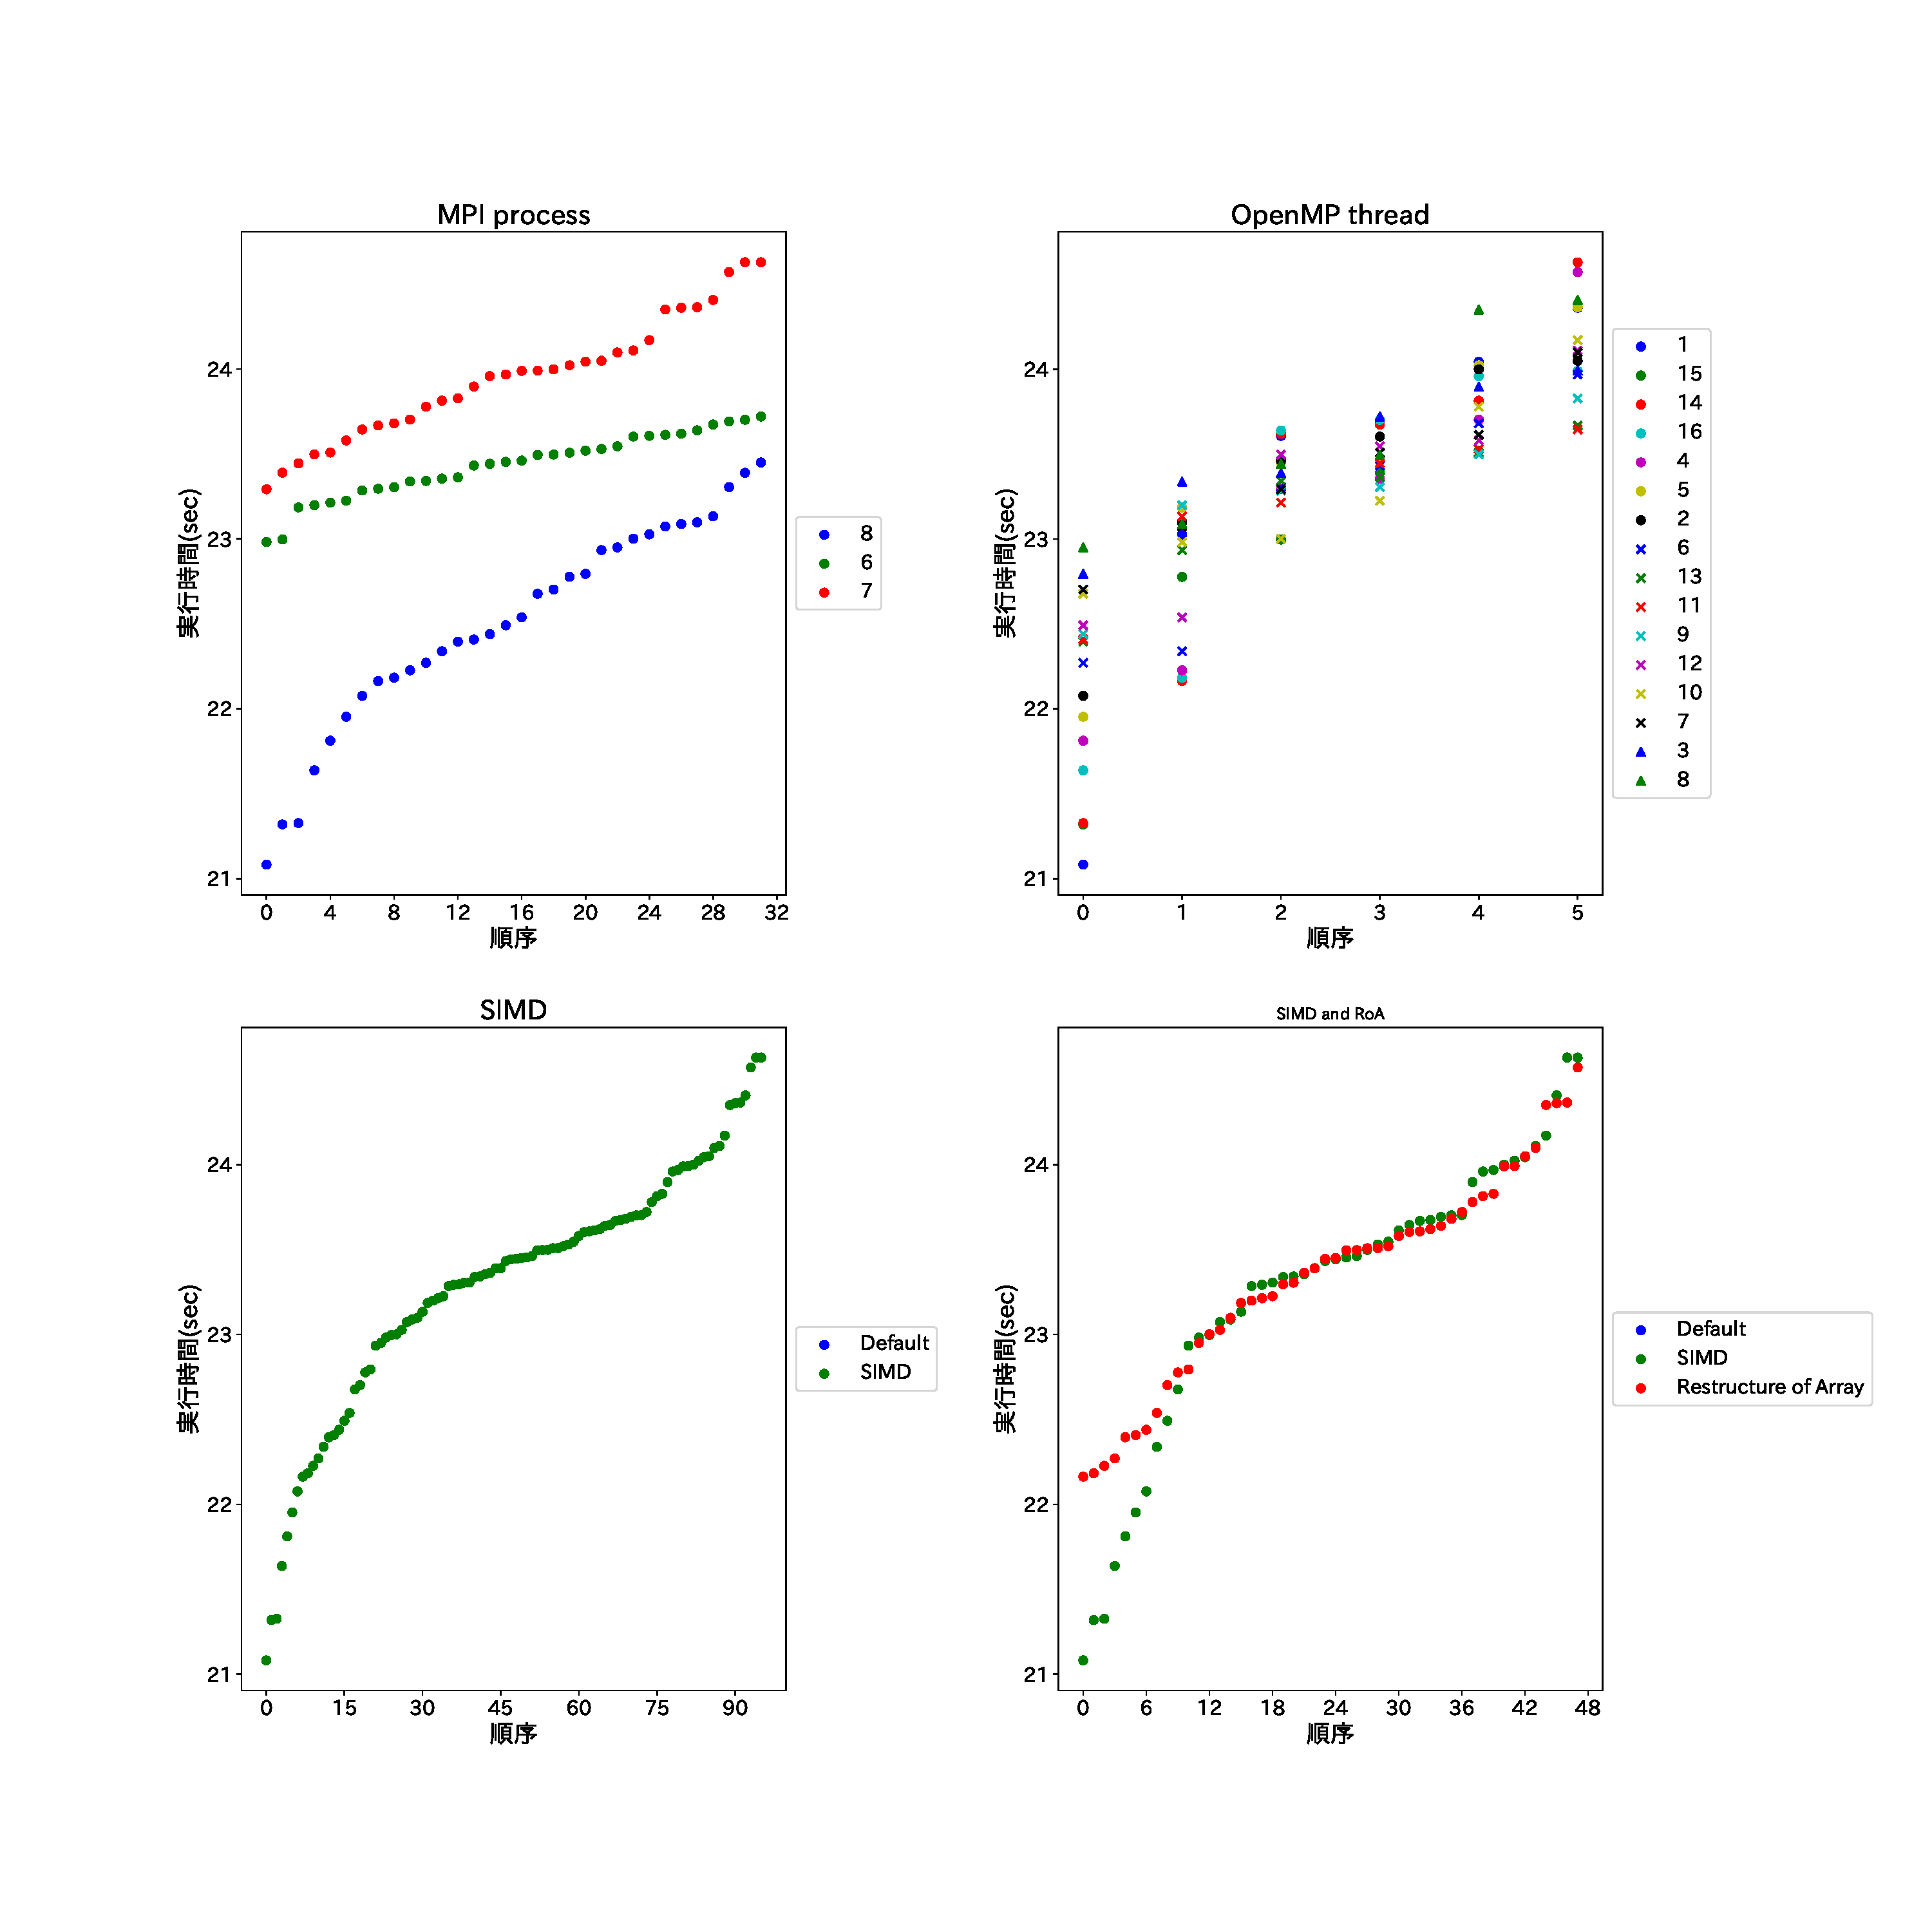
\includegraphics[width=14cm]{./images/k-bench-top25.pdf}
    \caption{京 小規模シミュレーション結果 top25\%}
    \label{fig:k-bench-top25}
\end{center}
\end{figure}

以下がクラスタと同様に京で小規模シミュレーションを元に絞り込みを行ったパラメータ候補である.\\
 クラスタと京の絞り込み後のパラメータから\ref{subsubsec:hybrid}項で述べたように,
小規模環境においてはMPIプロセスが最適化の中で大きな役割を果たすことがわかり,
コアのほとんどをMPIプロセスで利用する場合に高速になる傾向が強いことがわかった.\\
 また京において, 配列のくくり出しをしない方がより高速化されていることが図\ref{fig:k-bench-adjusted-final}の右下のグラフから読み取れるが,
これは京がアーキテクチャとしてSIMDに強く京で用いられるコンパイラもSIMDに適していることが原因であると推察される.
\begin{table}[htb]
  \caption {京でのパラメータ 絞り込み後}
  \begin{center}
    \begin{tabular}{|p{6cm}|p{8cm}|}
      \hline
      パラメータ & 値の範囲\\ \hline
      ノード数 & 8\\ \hline
      MPIプロセス数 & 8\\ \hline
      OpenMPスレッド数 & 1〜16\\ \hline
      SIMD化 & 行う\\ \hline
      配列のくくり出し & 行う(SIMD化を行っているならば) or 行わない\\ \hline
    \end{tabular}
  \end{center}
\end{table}

\begin{figure}[htb]
% h:here, t:top, b:bottom, p:page
\begin{center}
%    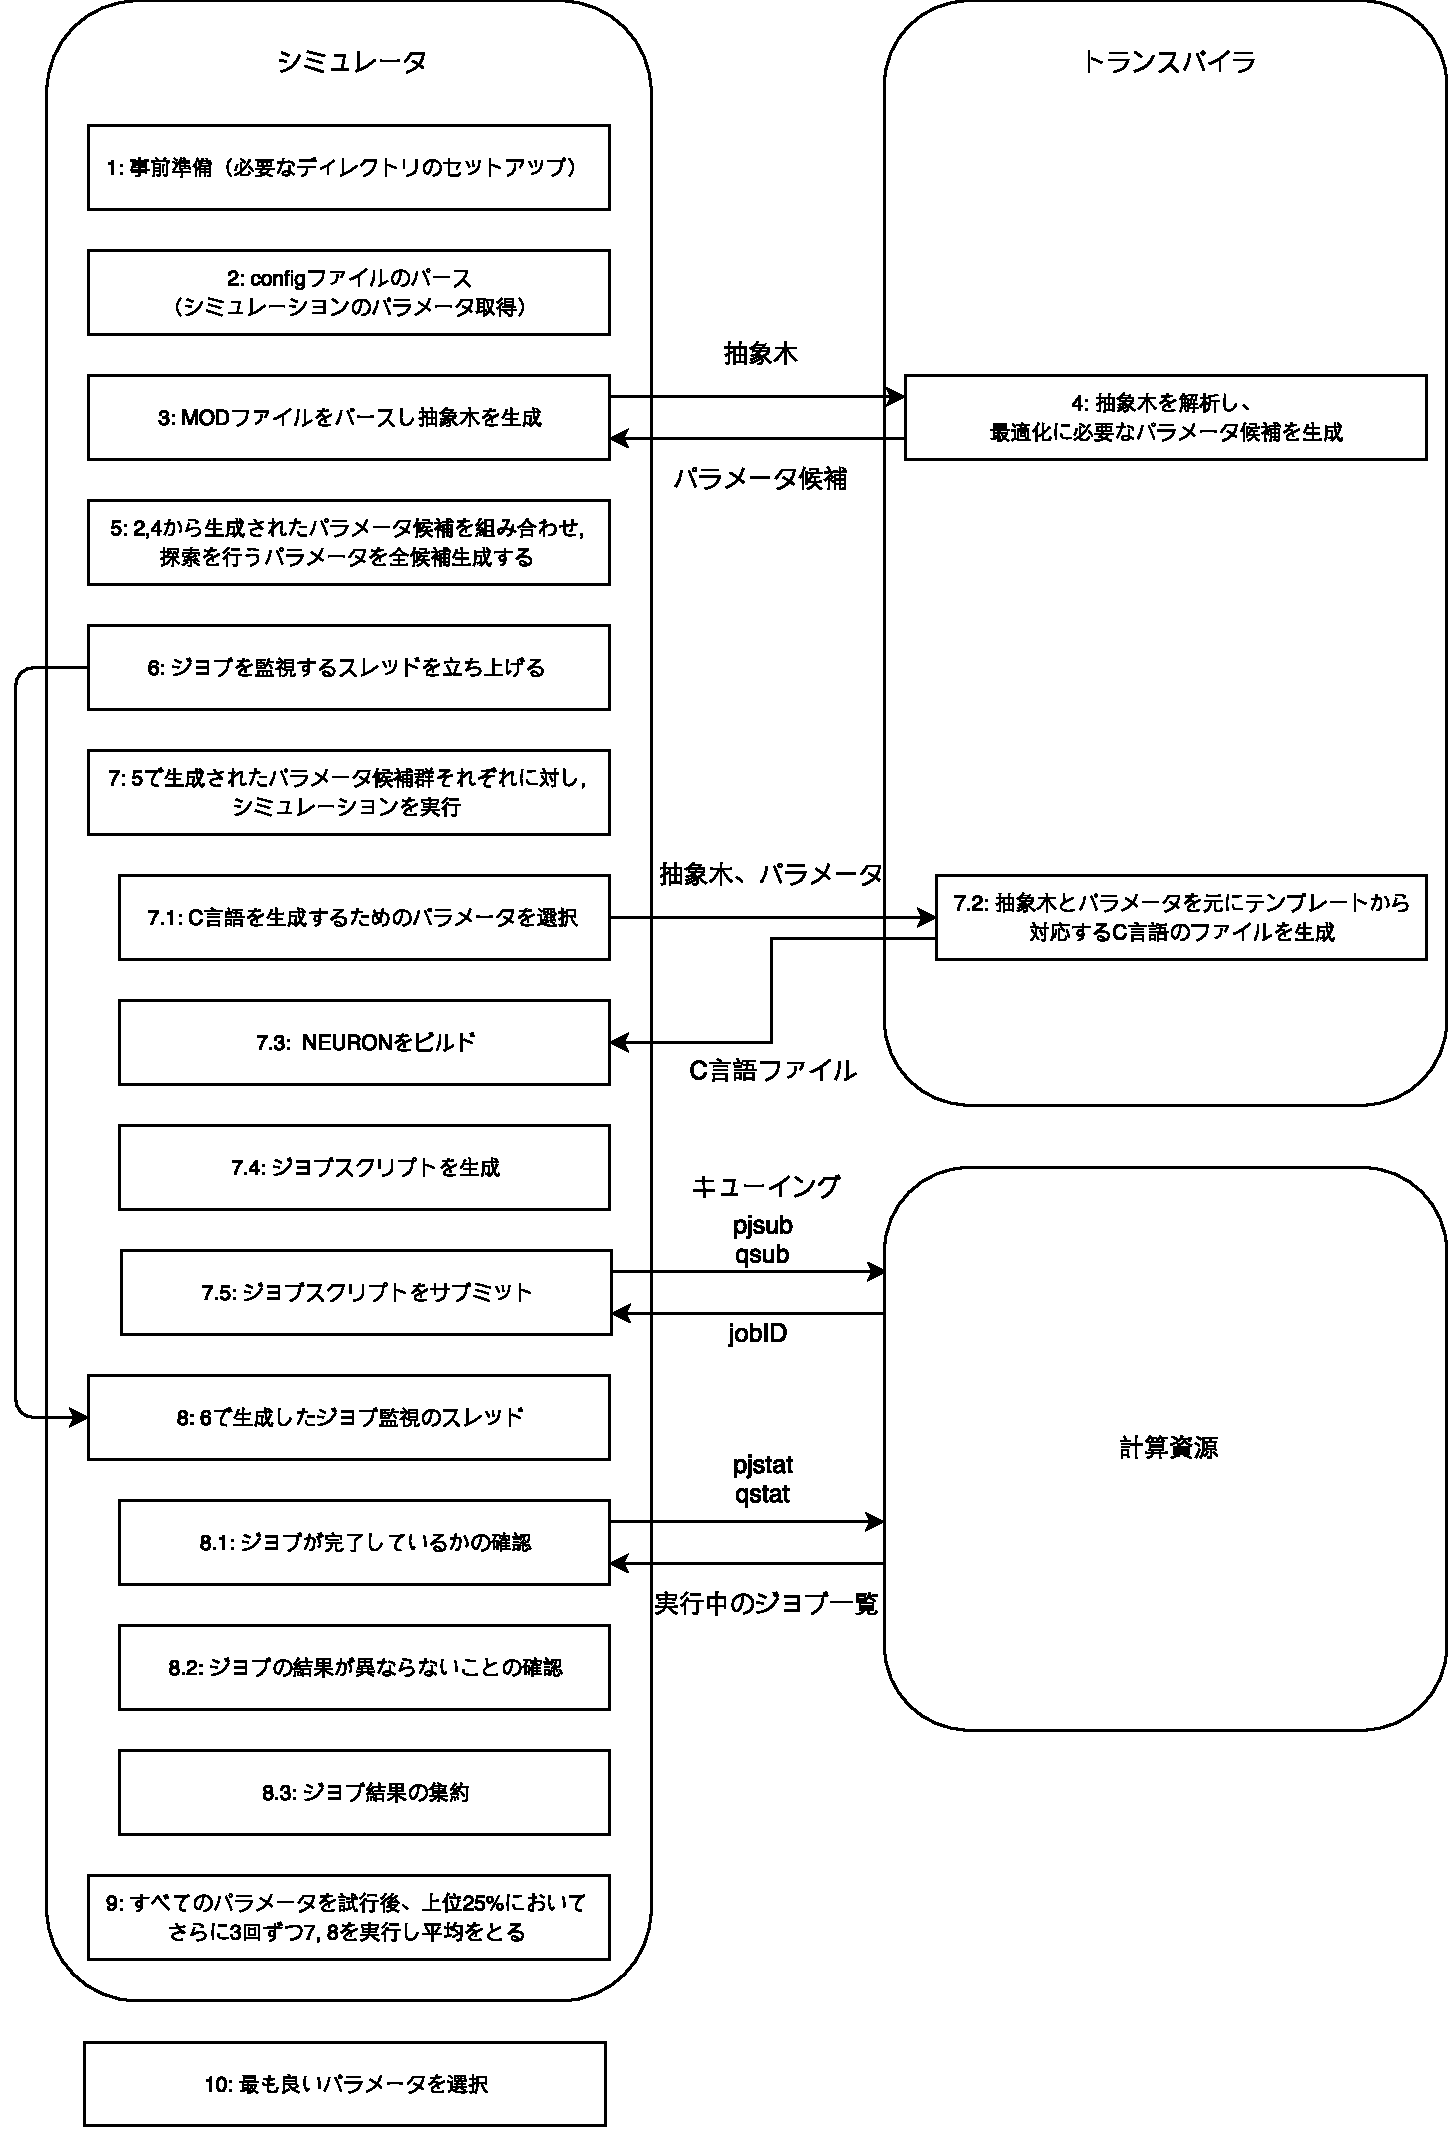
\includegraphics[width=18.0cm]{./images/Genie.pdf}
    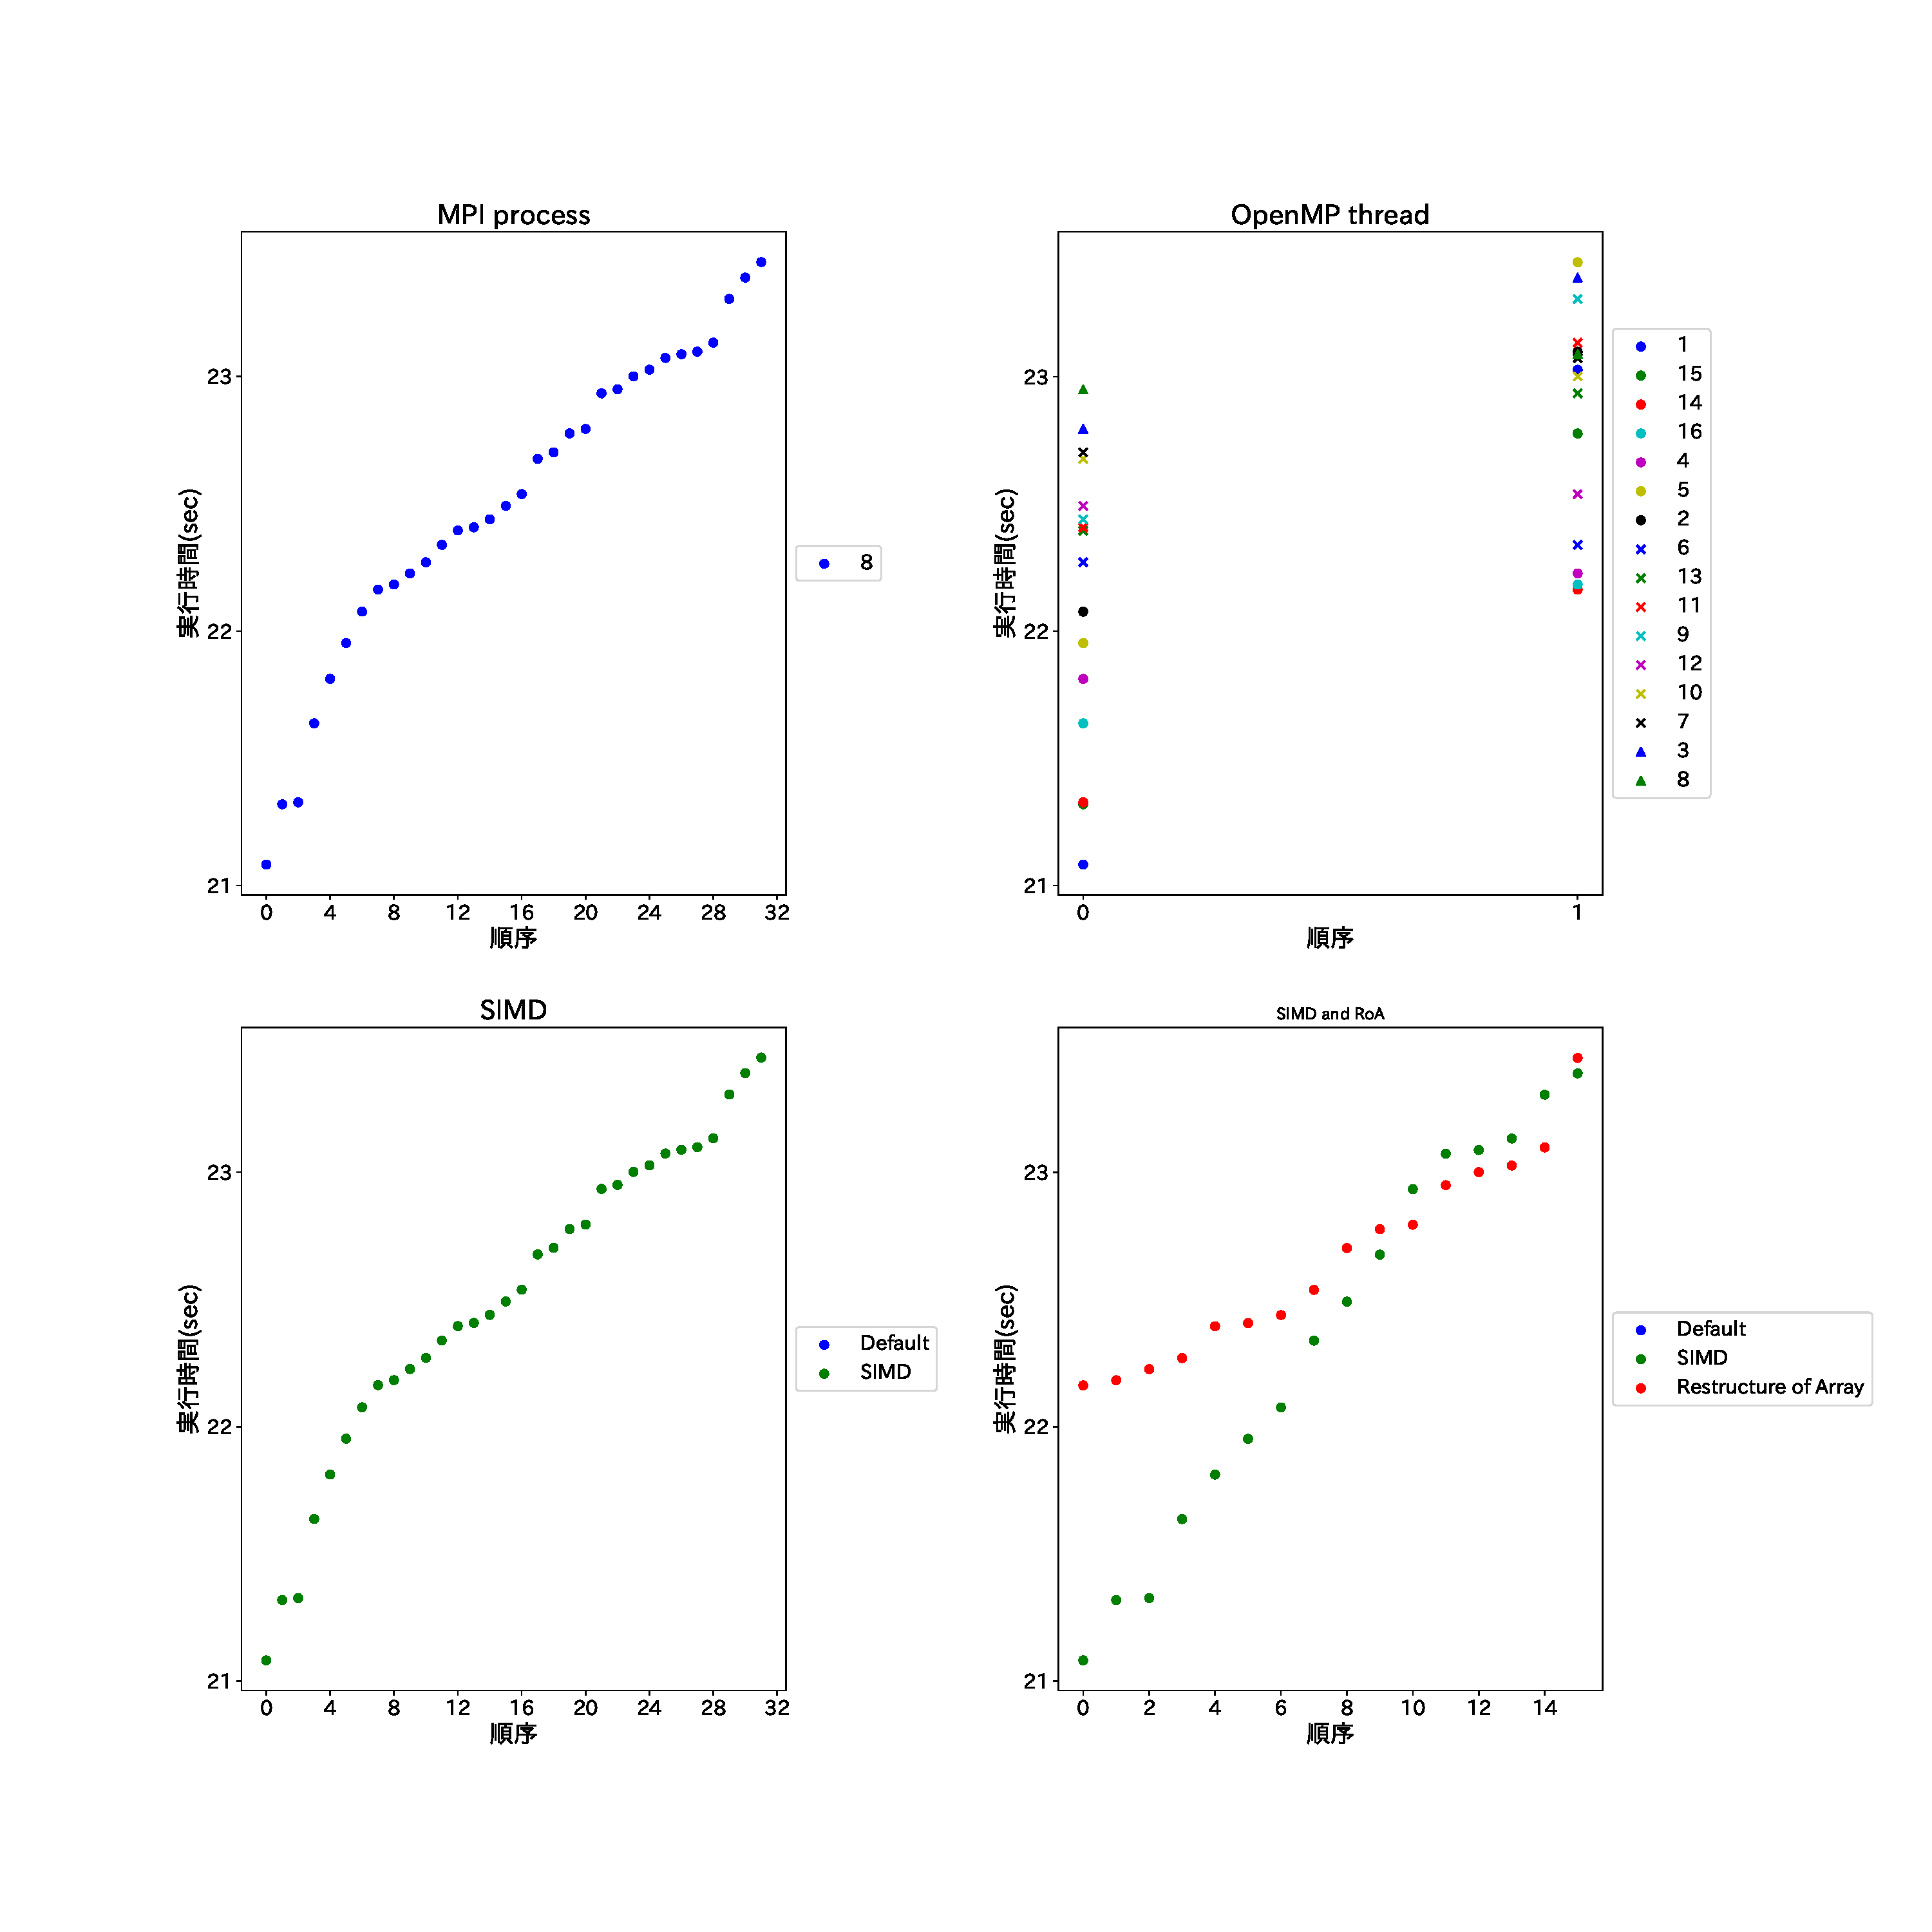
\includegraphics[width=14cm]{./images/k-bench-adjusted-final.pdf}
    \caption{京 小規模シミュレーション結果 パラメータ絞り込み後}
    \label{fig:k-bench-adjusted-final}
\end{center}
\end{figure}
\clearpage
次に小規模のシミュレーションを通して絞り込んだパラメータを用いて,
実行時間と反復する回数を変えてシミュレーションを再度行い,
実行時間とパラメータの関係を調べる.\\

\subsection{詳細なシミュレーションでのパラメータ比較}
\label{subsec:detail-sim}
ここでは\ref{subsec:small-sim}節において絞り込みを行ったパラメータを用い,
京, クラスタそれぞれにおいて実行時間を50, 100, 250, 500, 1000msとして6回シミュレーションを行いその実行時間の平均をとることで,
より詳細にパラメータの比較を行った.
尚, SIMD化については\ref{subsec:small-sim}節において既にSIMD化を行わないパラメータは除外されているためここでは触れない.
また, 京においてはMPIプロセス数に関しても除外されているため同様な扱いとする.\\

\subsubsection{MPIプロセス数}
\paragraph{クラスタ}~\\
図\ref{fig:cluster-mpi-process}のプロセス数に注目すると, プロセス数が28の時を除きシミュレーション時間を長くしてもMPIプロセス数間の関係に変化は見られない.\\
クラスタにおいてはコア数が28であることから,
シミュレーション時間が最大で1000msと短く細胞数も少ない今回のような場合においてはMPIプロセスでコアを埋めきるほうが計算性能が高くなることが読み取れる.\\
\begin{figure}[htb]
% h:here, t:top, b:bottom, p:page
\begin{center}
%    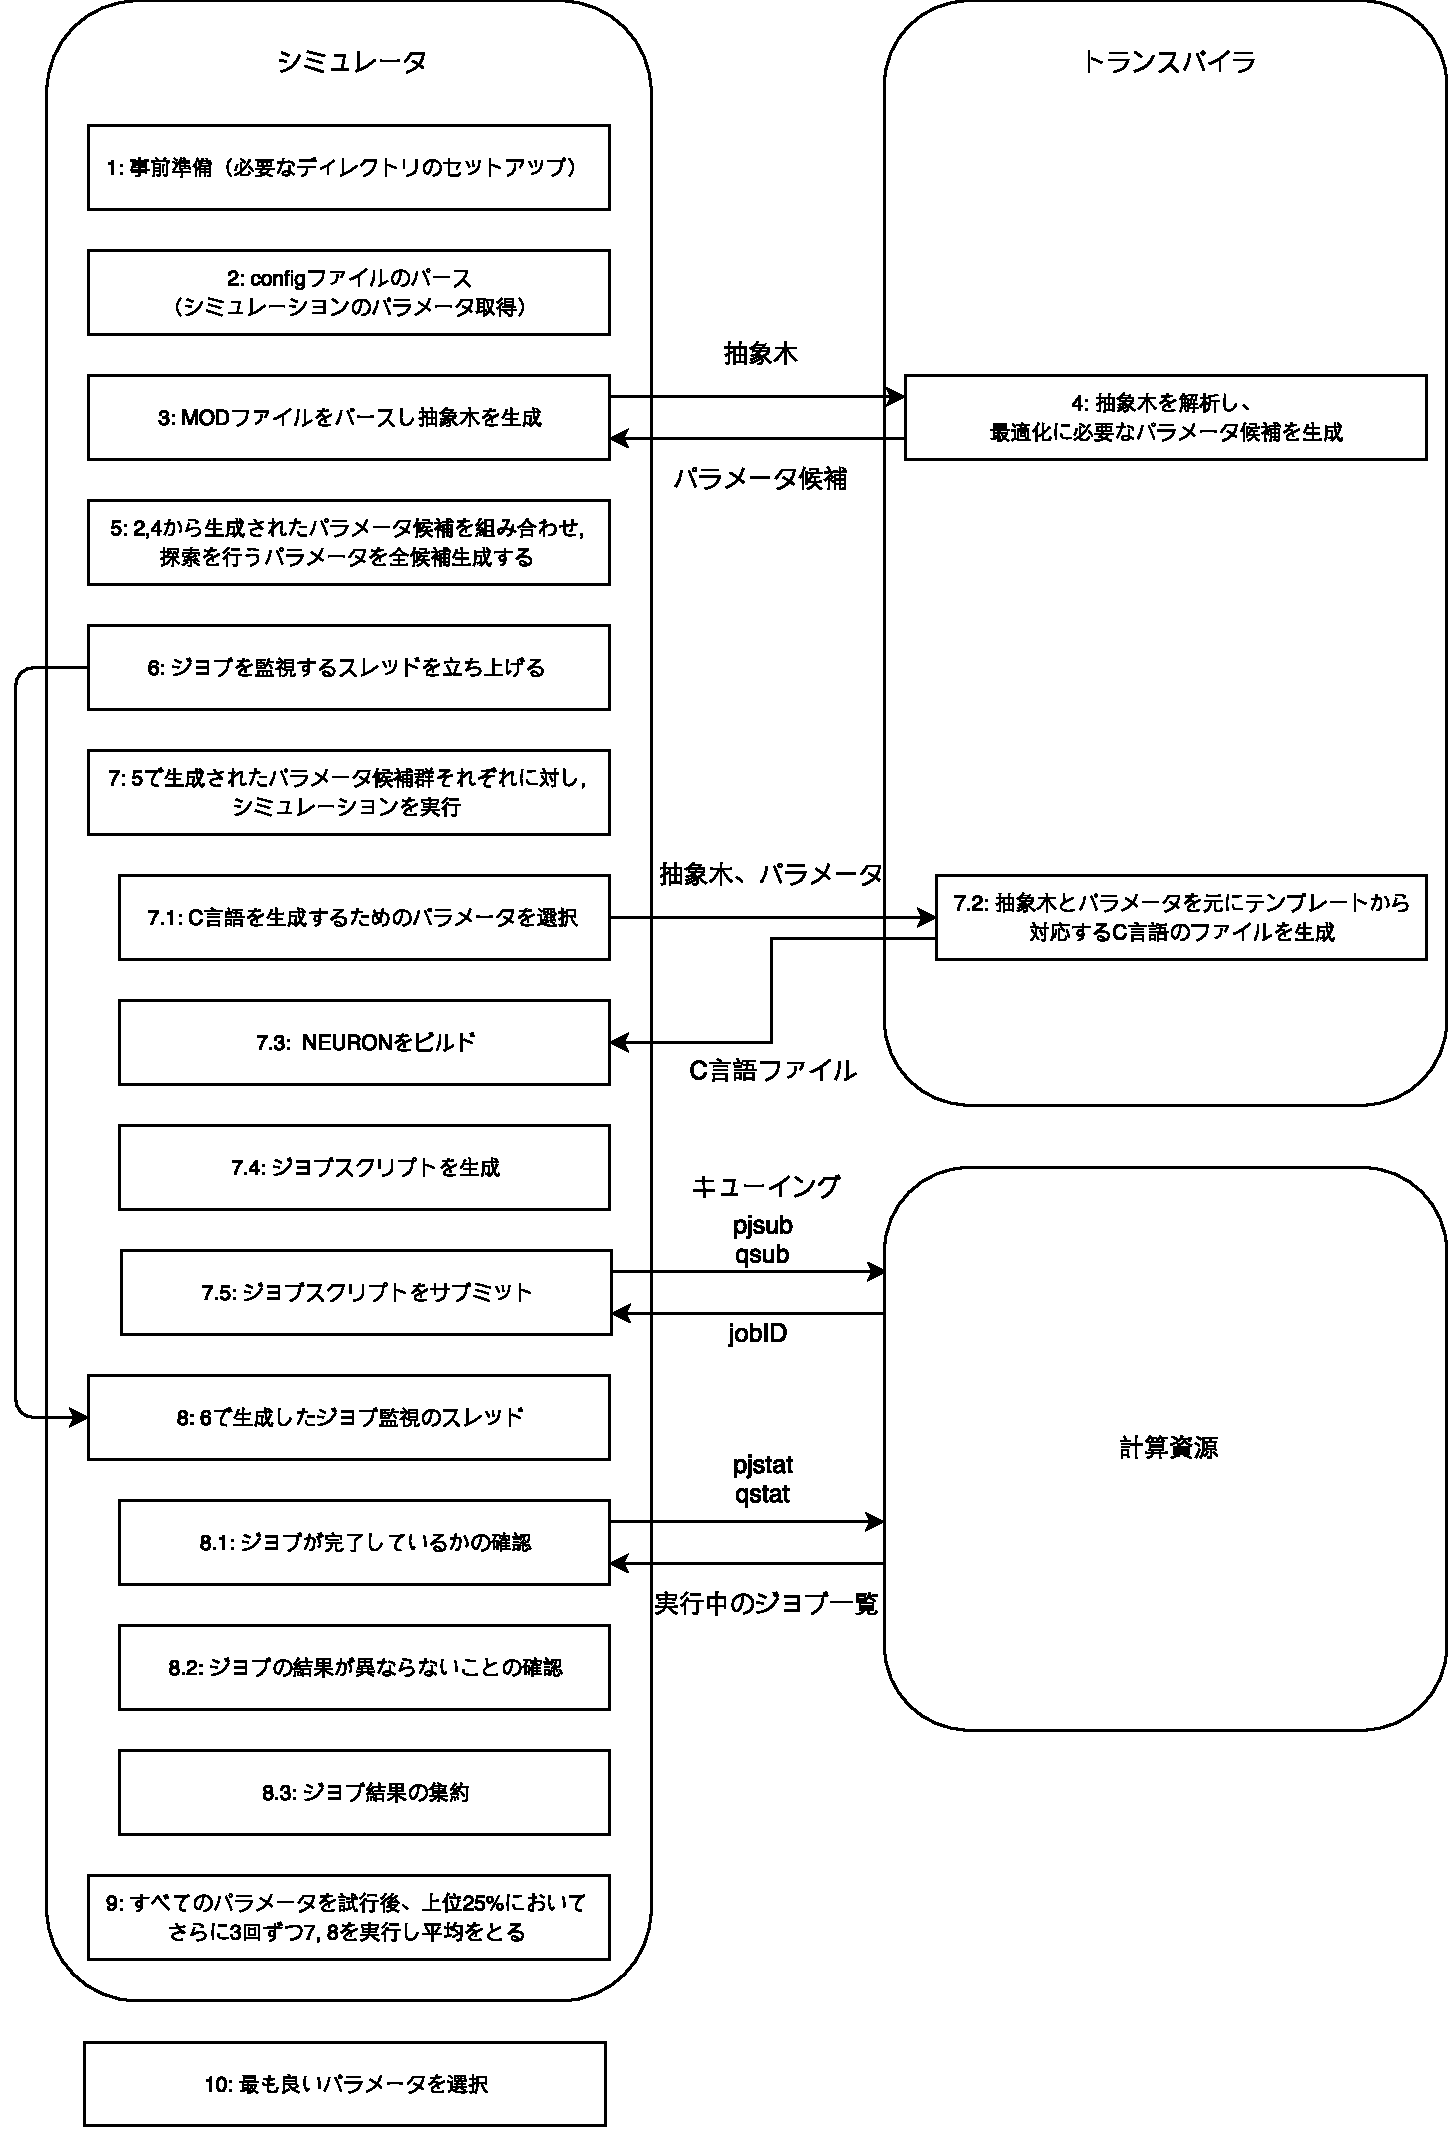
\includegraphics[width=18.0cm]{./images/Genie.pdf}
    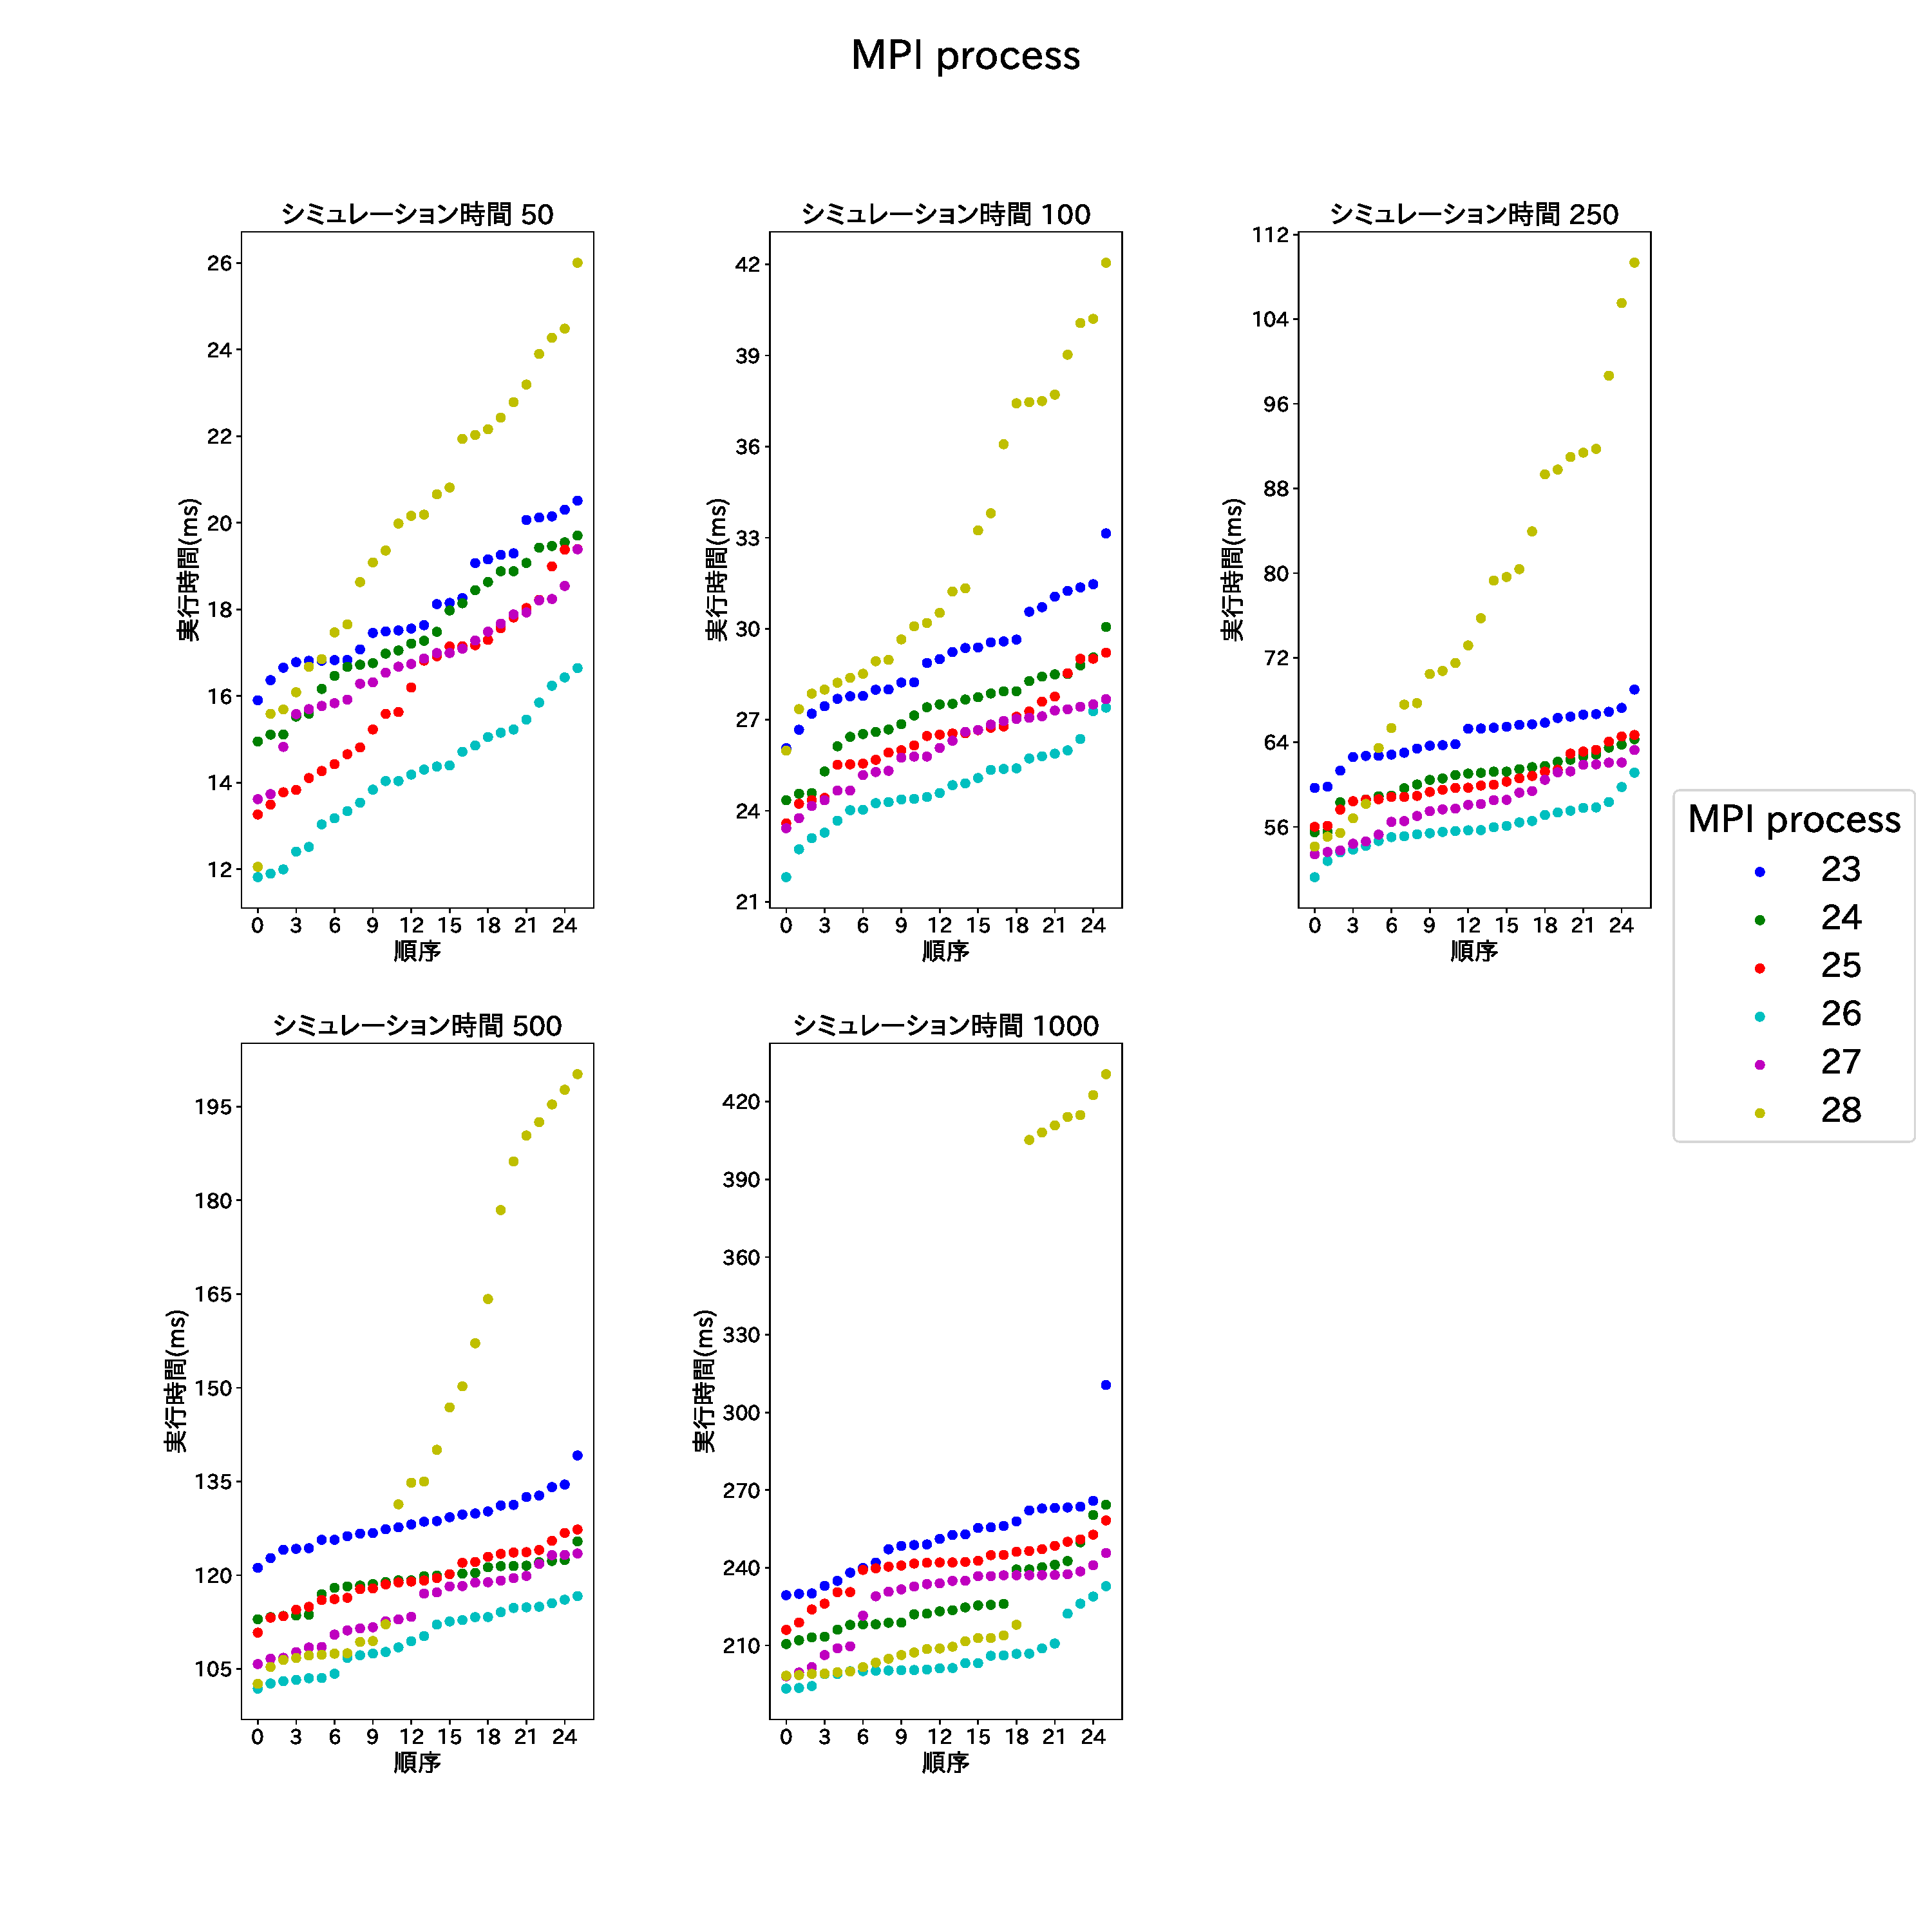
\includegraphics[width=12cm]{./images/cluster-MPI-process.pdf}
    \caption{クラスタ MPIプロセス数 シミュレーション結果}
    \label{fig:cluster-mpi-process}
\end{center}
\end{figure}
\clearpage

\subsubsection{OpenMPスレッド数}
\paragraph{クラスタ}~\\
OpenMPスレッドについては他のパラメータと違いスレッド数の間で大きな差が見られない傾向にあったため,
図\ref{fig:cluster-openmp}のように折れ線グラフを用いてどの程度混在しているのか確認した.\\

\begin{figure}[htb]
% h:here, t:top, b:bottom, p:page
\begin{center}
%    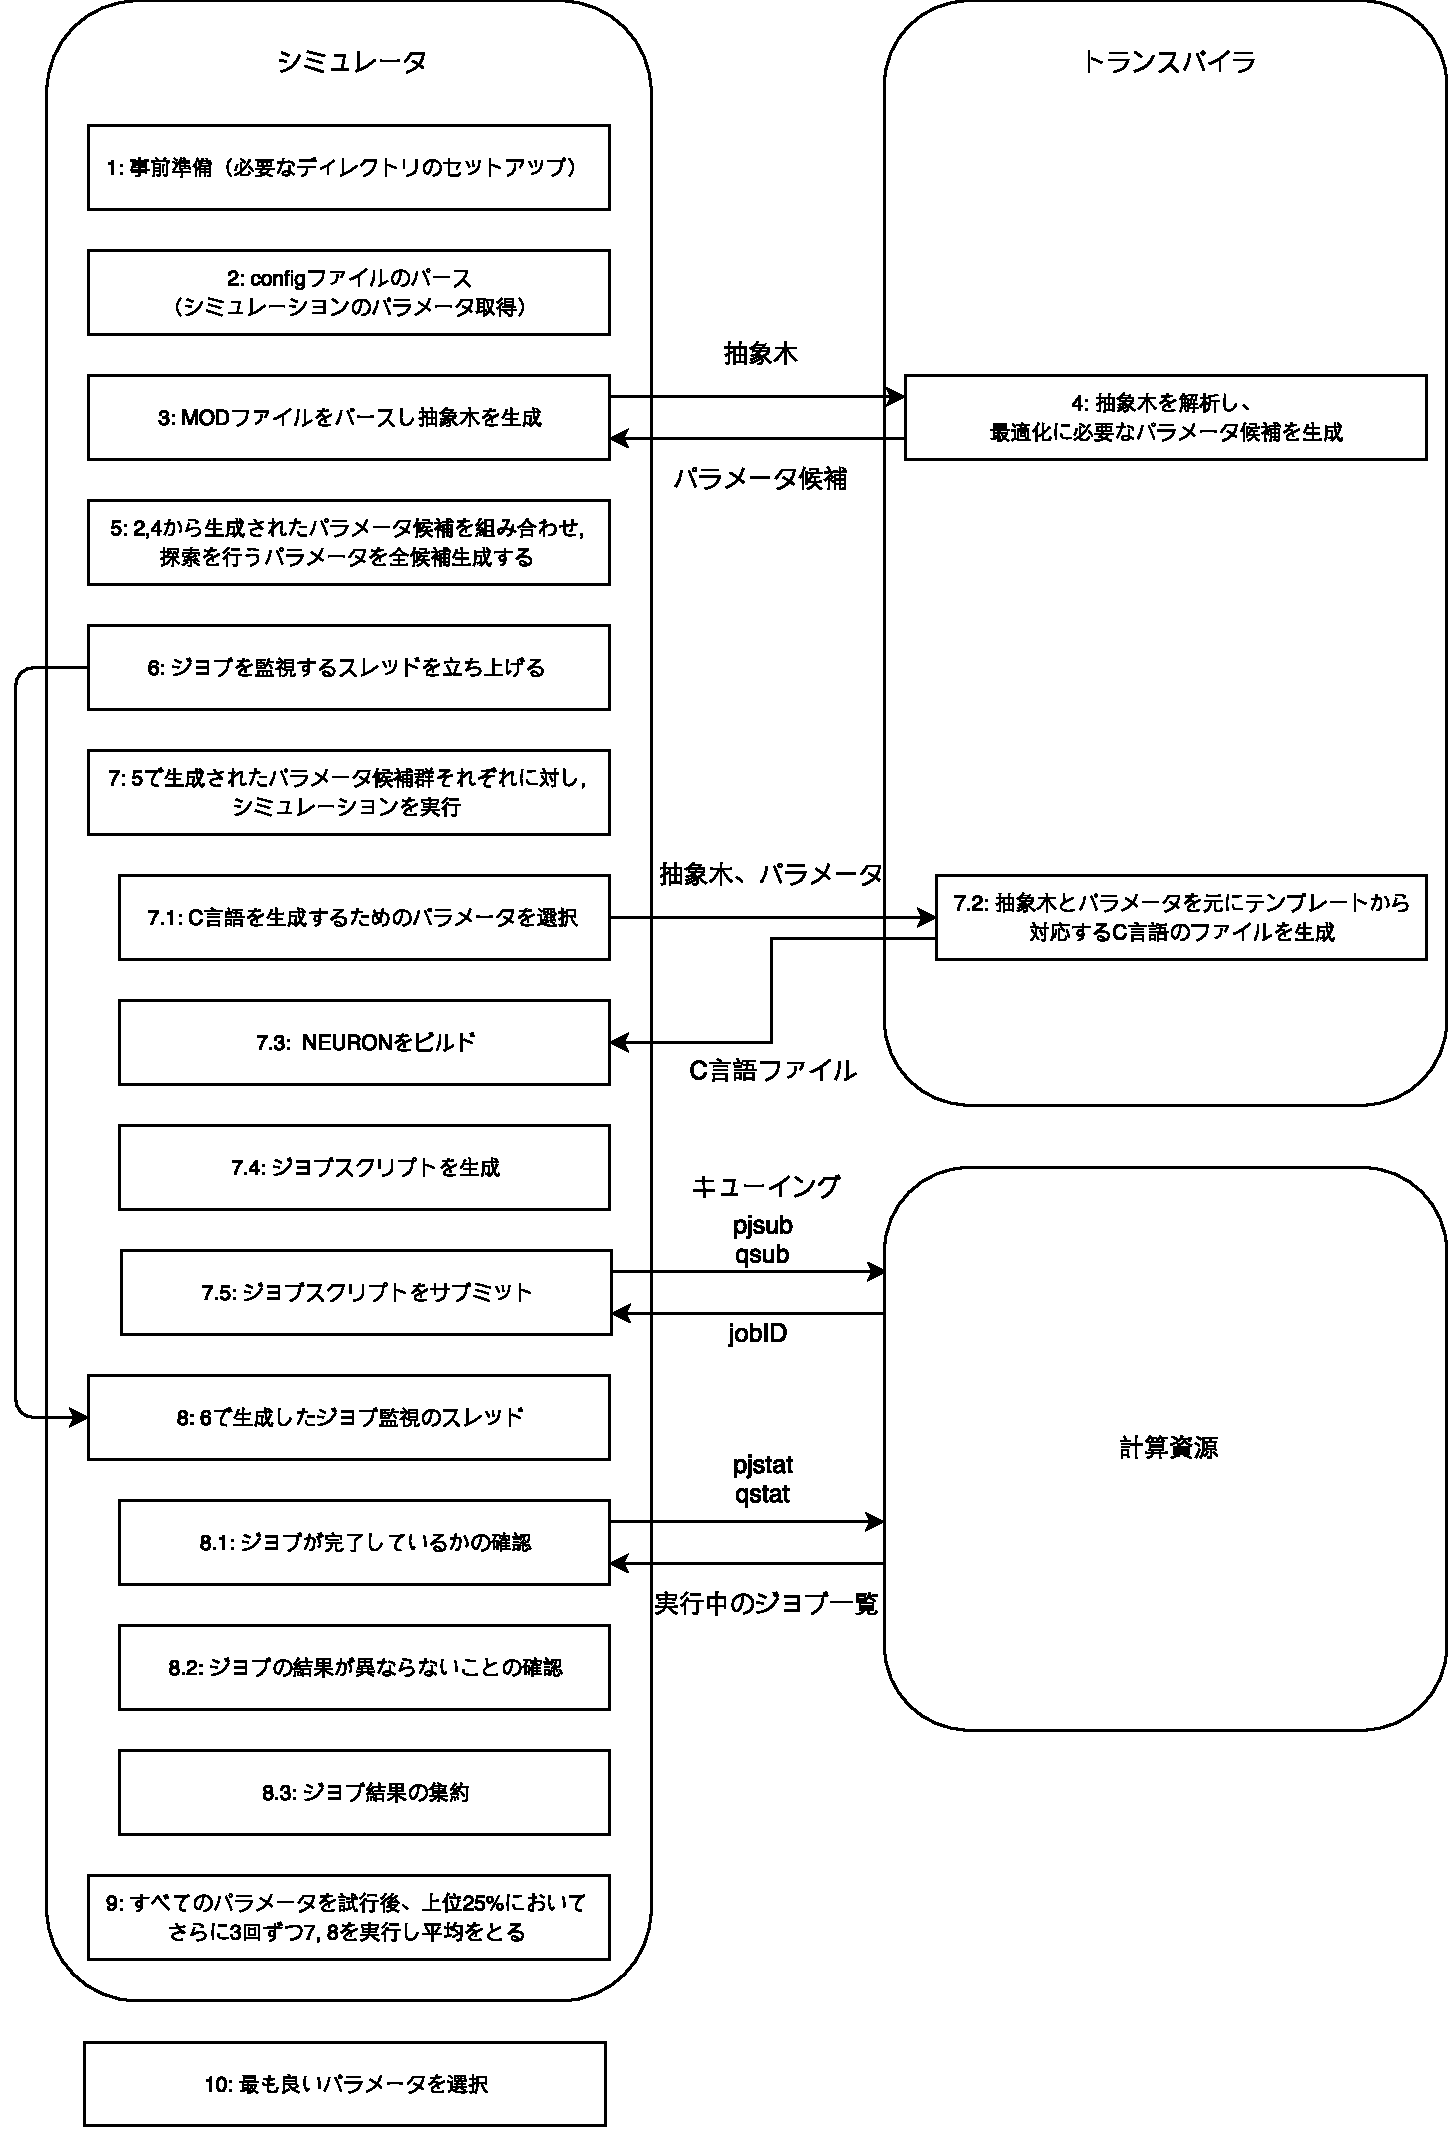
\includegraphics[width=18.0cm]{./images/Genie.pdf}
    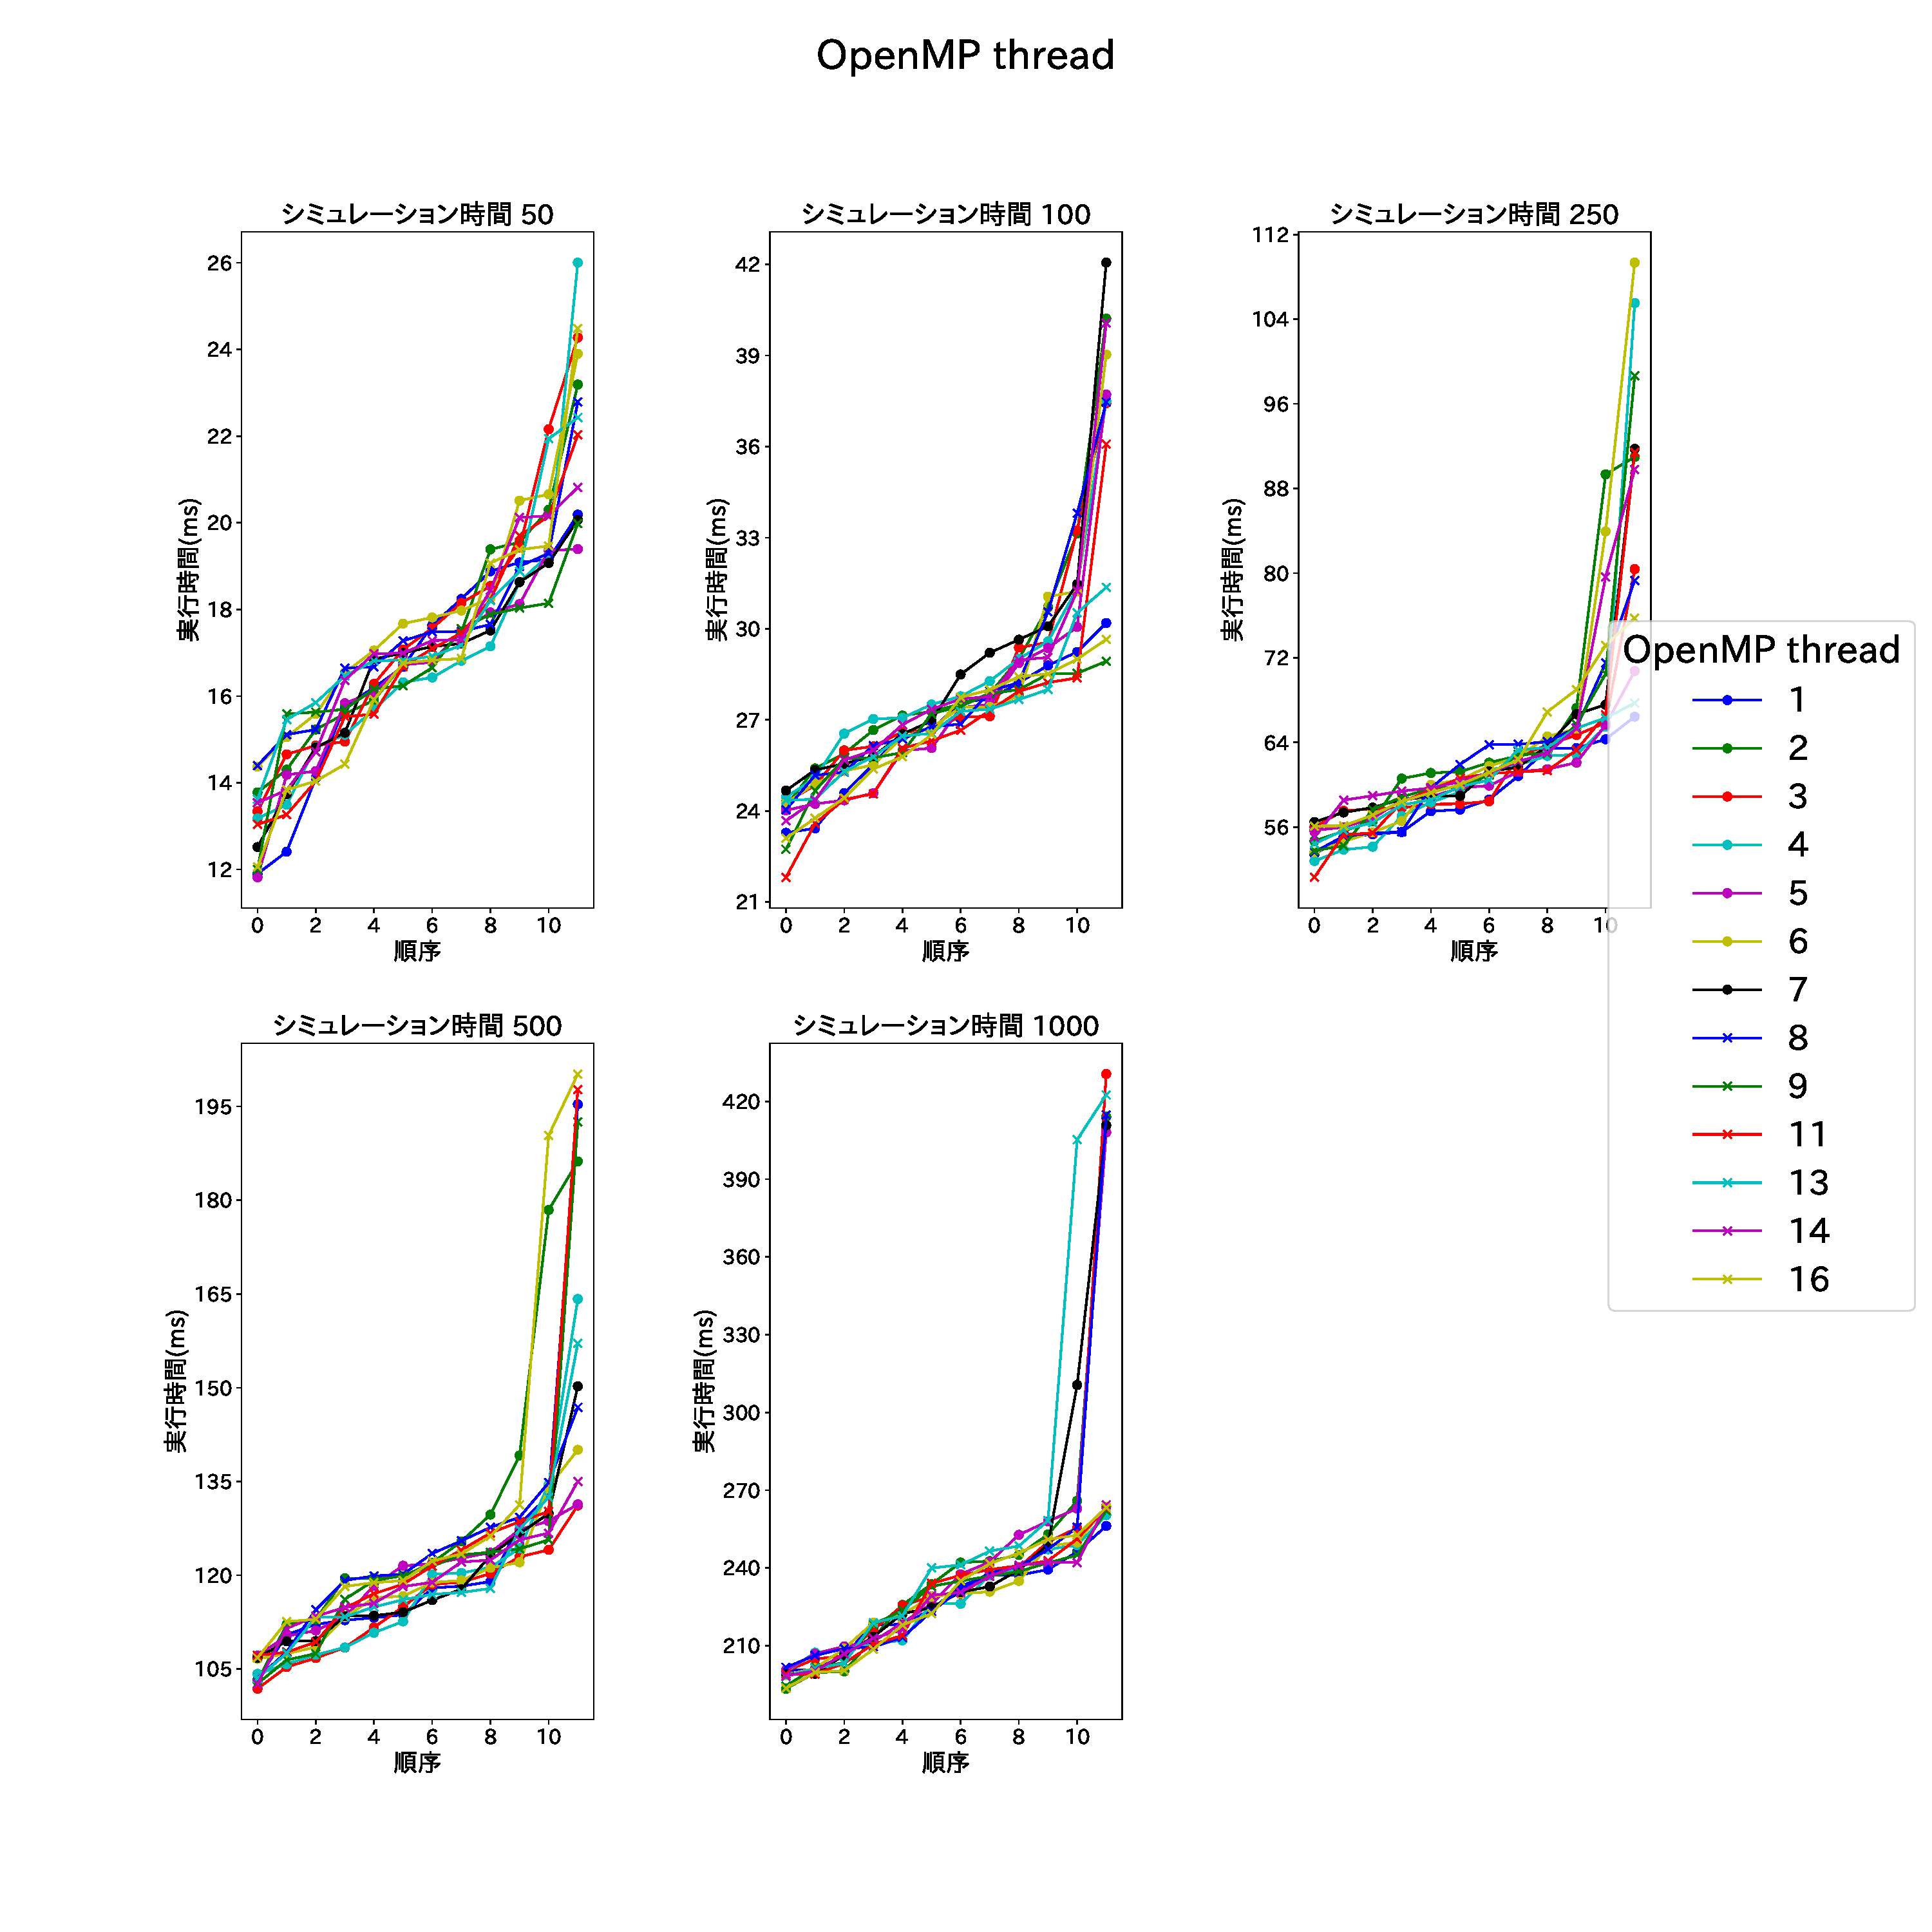
\includegraphics[width=14cm]{./images/cluster-OpenMP-thread.pdf}
    \caption{クラスタ OpenMPスレッド数 シミュレーション結果}
    \label{fig:cluster-openmp}
\end{center}
\end{figure}

図\ref{fig:cluster-openmp}において表示されるデータ点が多すぎるため,
データ点の数を50個に制限したものを次の図\ref{fig:cluster-openmp-top50}に示す.\\
\begin{figure}[htb]
% h:here, t:top, b:bottom, p:page
\begin{center}
%    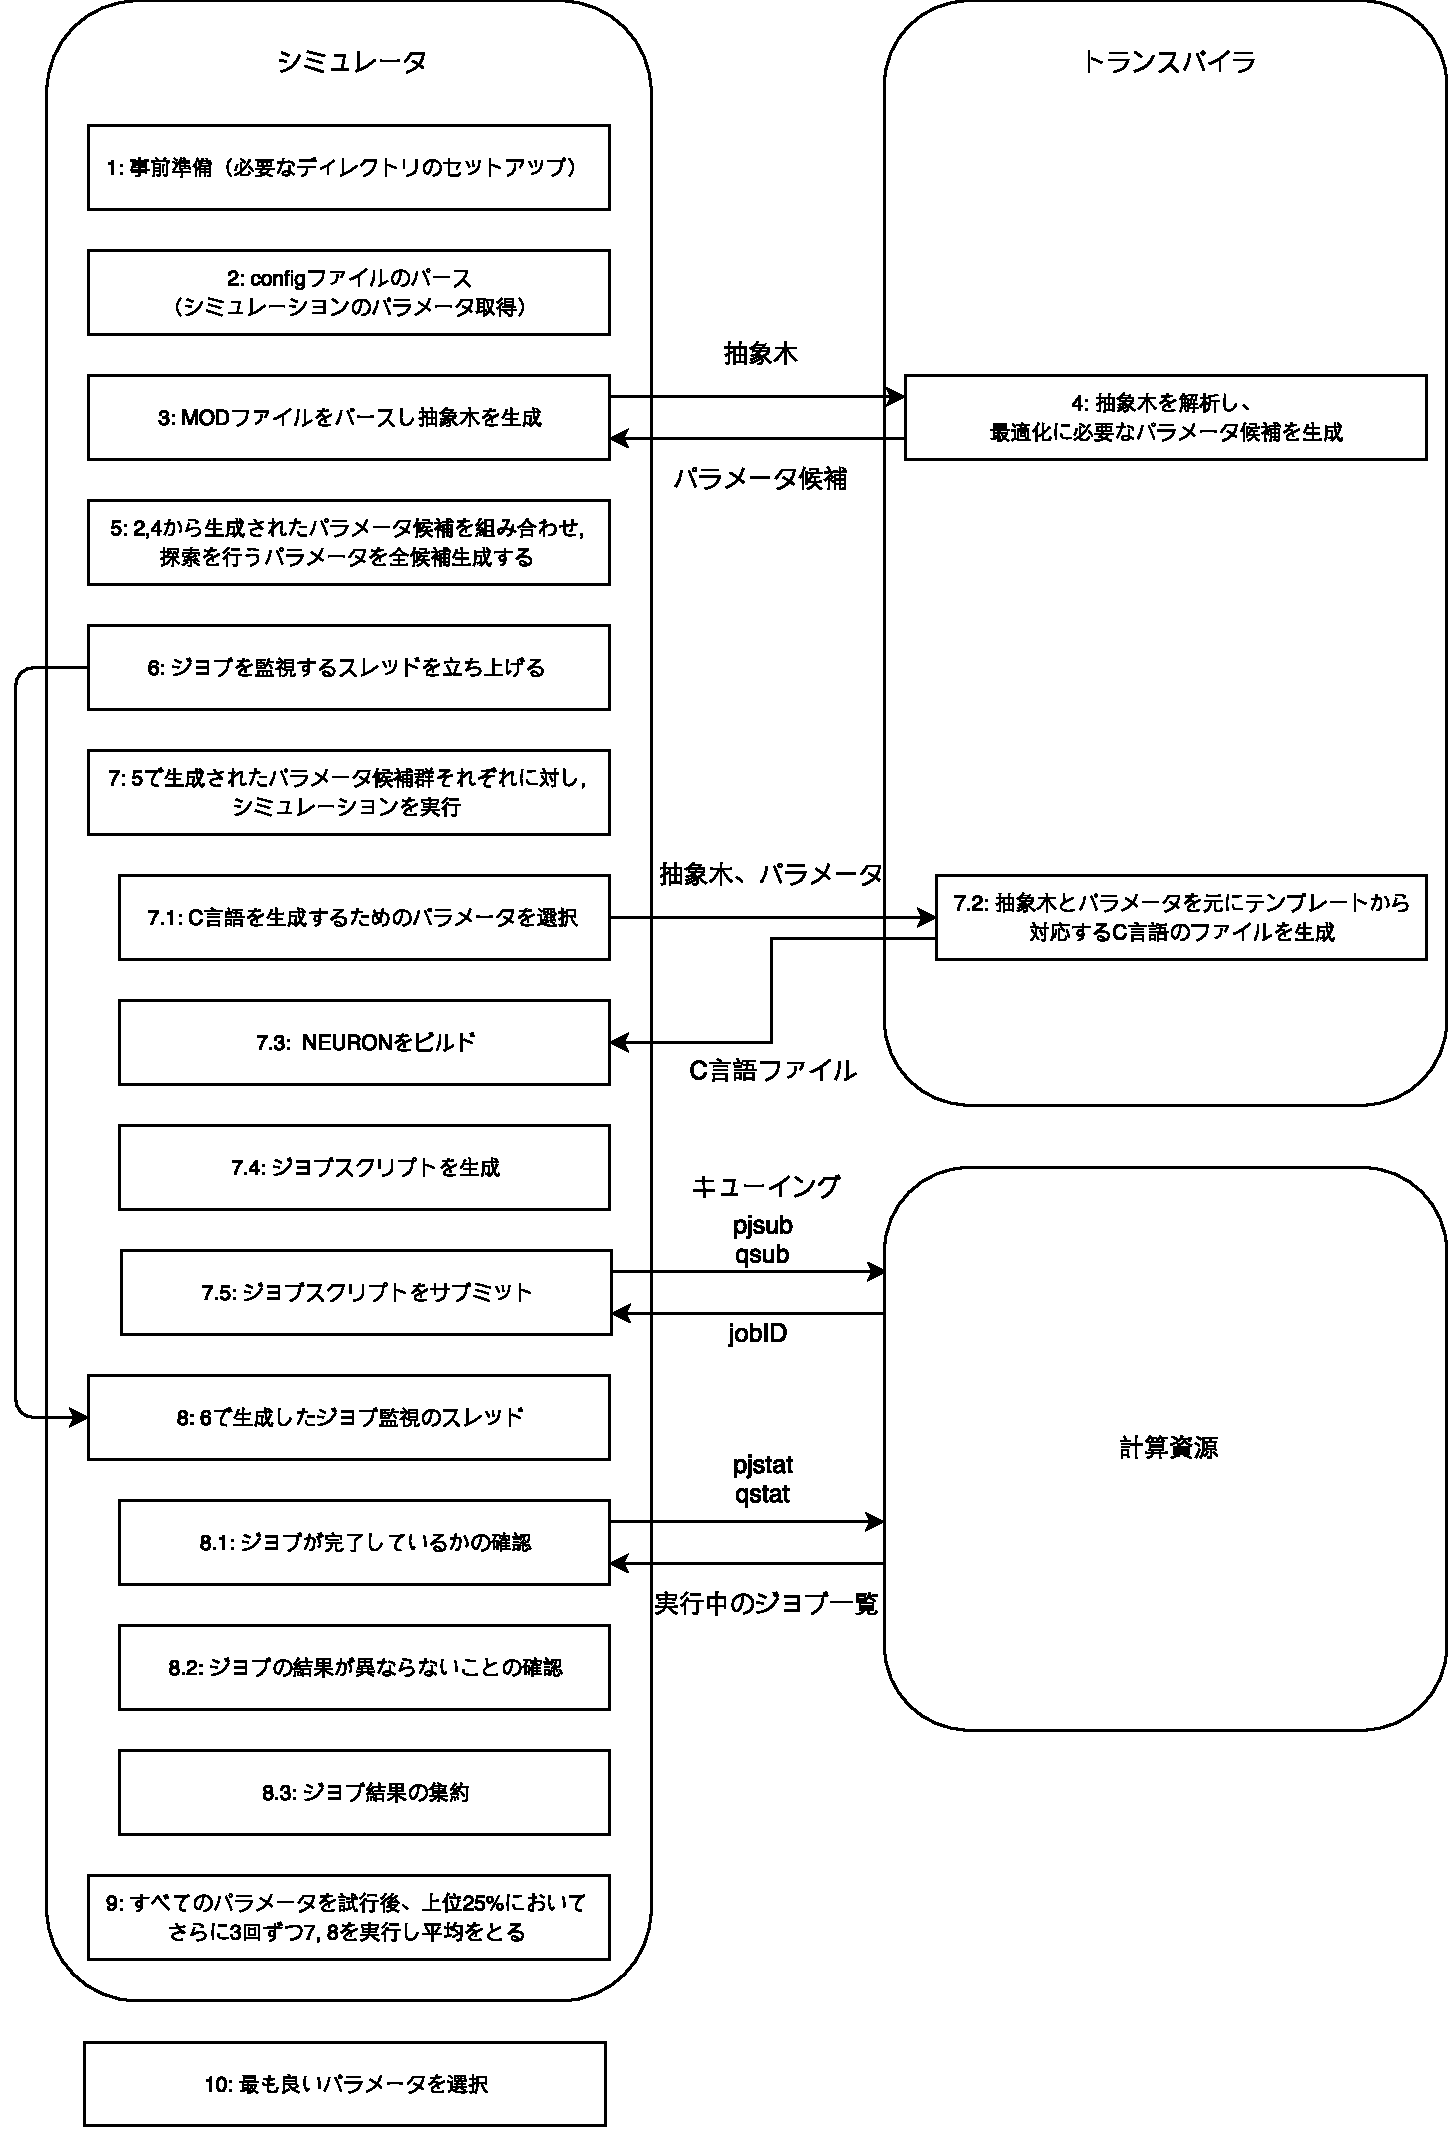
\includegraphics[width=18.0cm]{./images/Genie.pdf}
    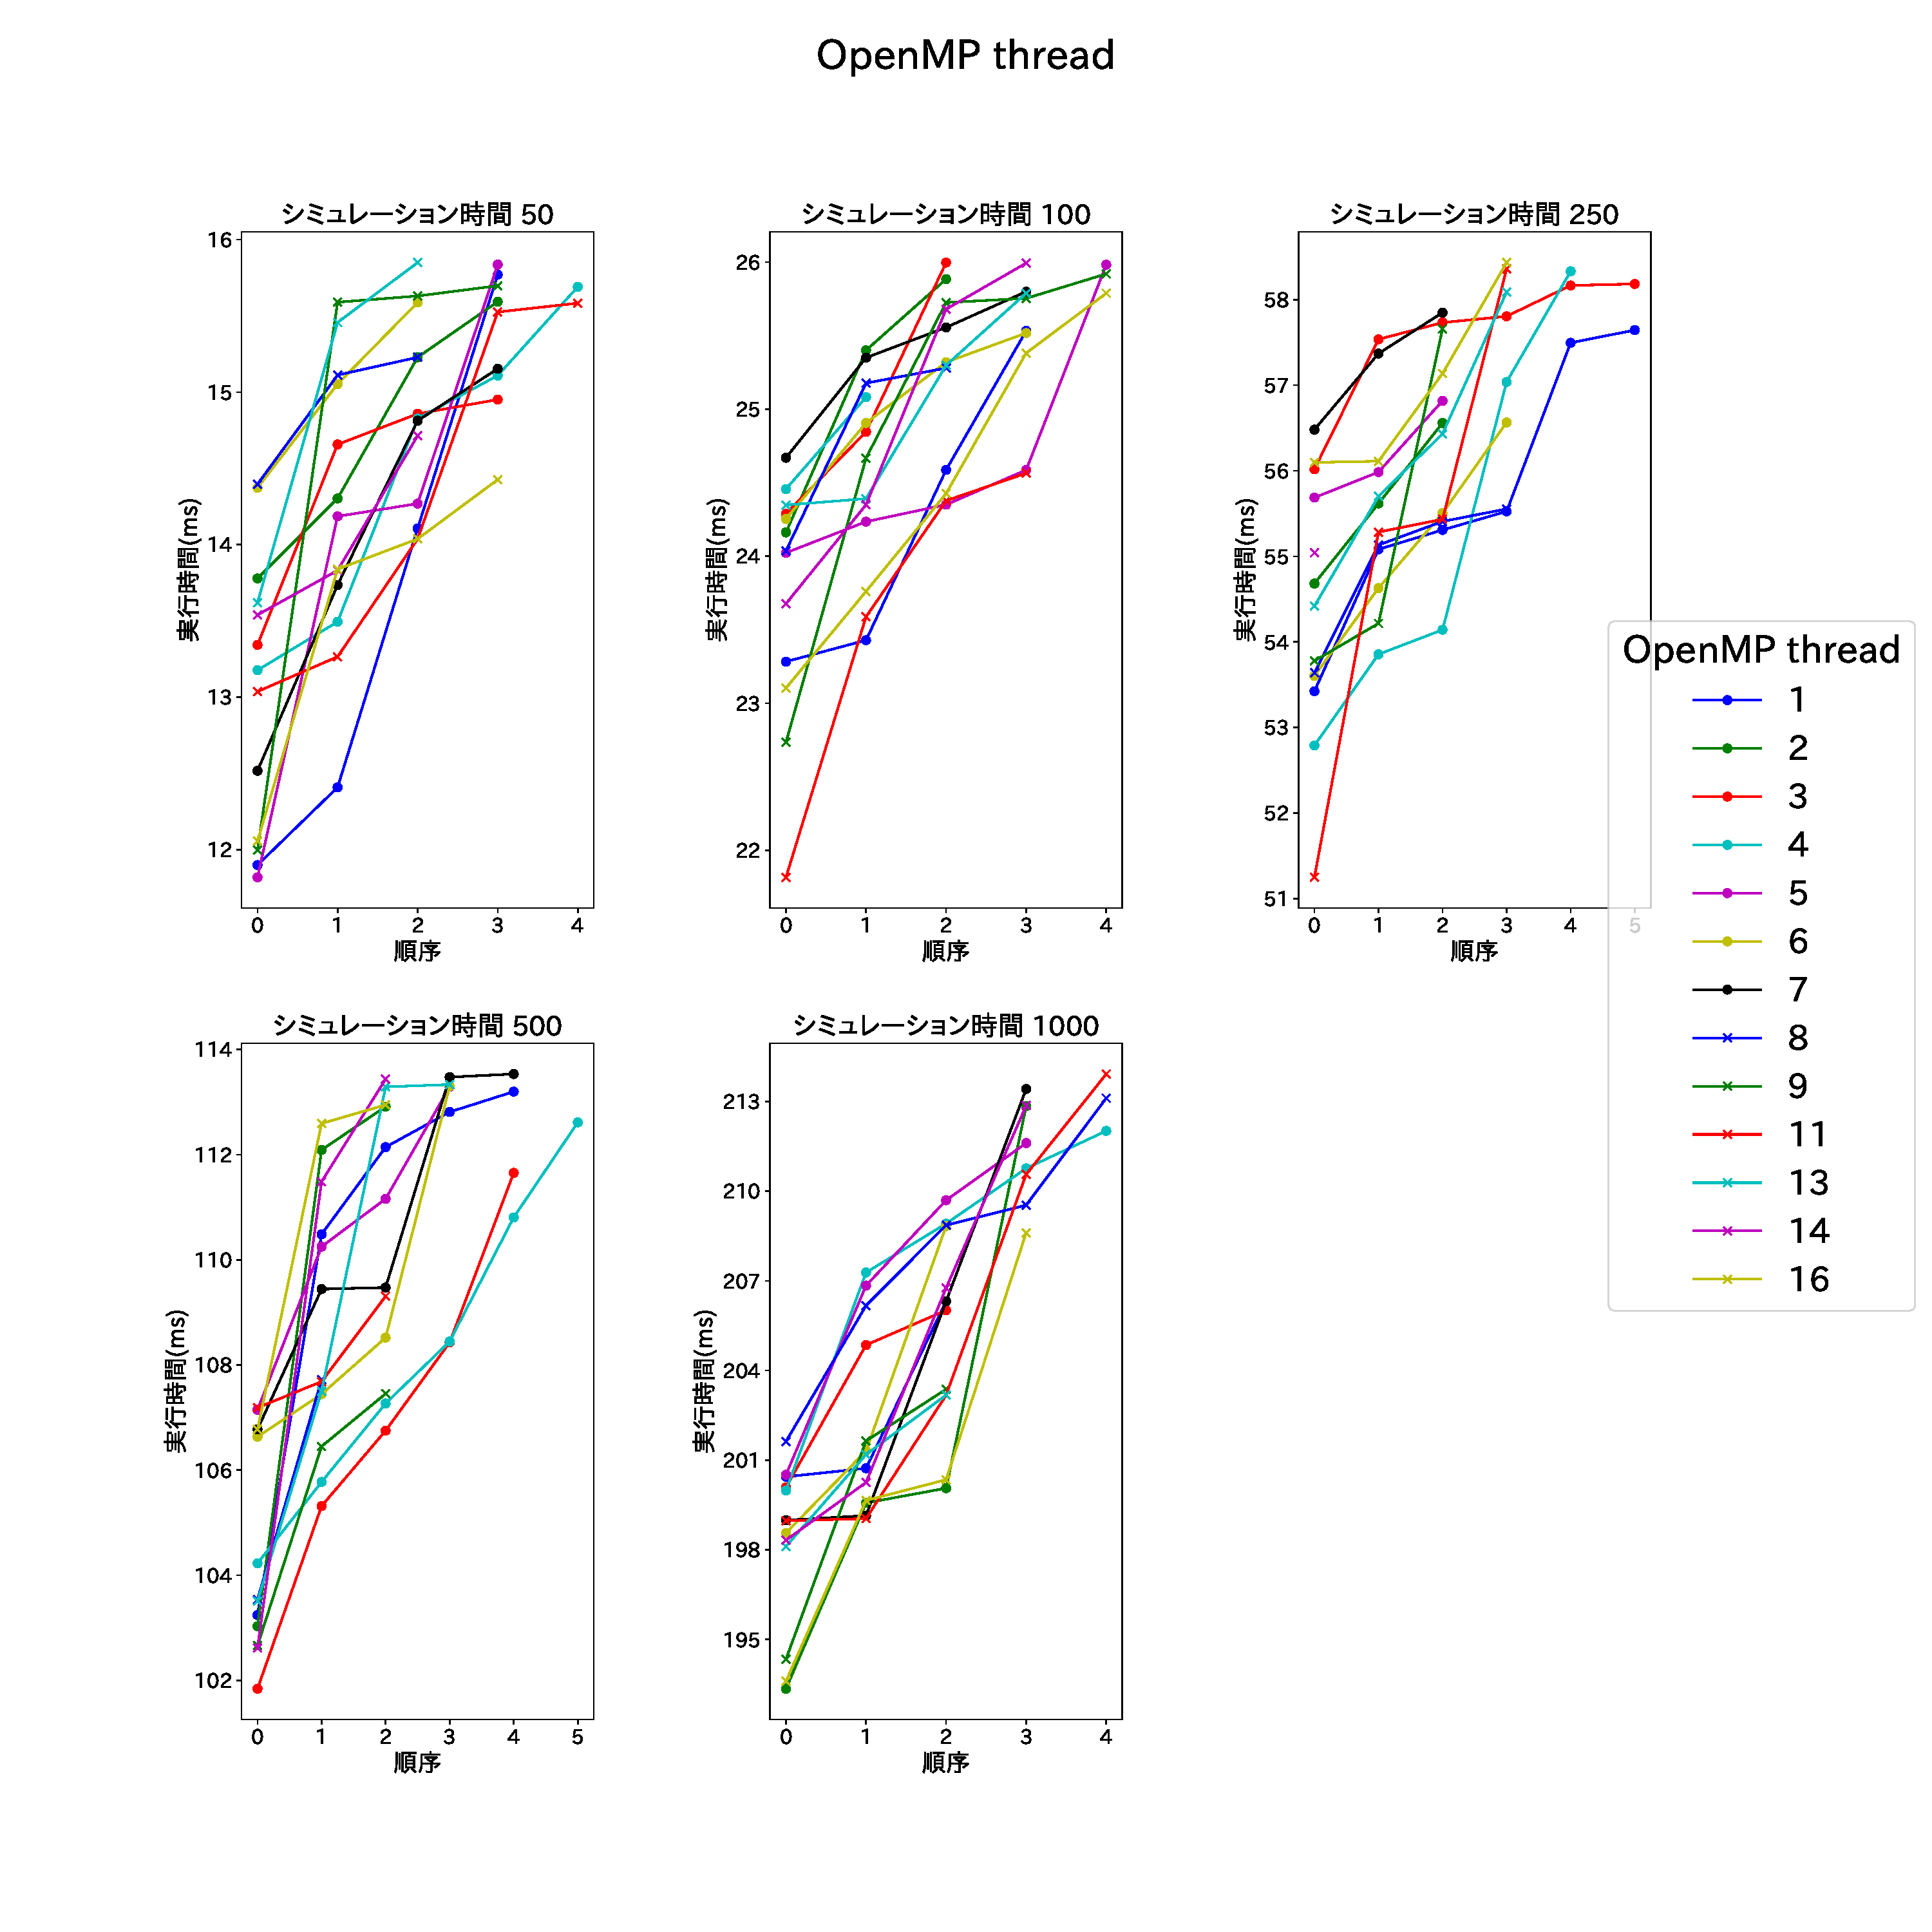
\includegraphics[width=14cm]{./images/cluster-top50-OpenMP-thread.pdf}
    \caption{クラスタ OpenMPスレッド数 シミュレーション結果 上位50組}
    \label{fig:cluster-openmp-top50}
\end{center}
\end{figure}
\clearpage
結果として, データ点を制限して表示した図においてもスレッド数と実行時間の直接的な相関を見ることができなかった.
これは\ref{subsubsec:hybrid}において述べたMPIとOpenMPのハイブリッドという観点では,
シミュレーションの規模が小さくMPIプロセスが通信に用いるリソースが十分に存在したため,
MPIによってコアを埋めた後ではOpenMPのスレッド数をいくつに設定しても実行時間に与える影響が少ないためだと考えられる.\\
\paragraph{京}~\\
クラスタ同様京においてもOpenMPスレッド数と実行時間の直接的な相関を見ることはできなかった.\\
\begin{figure}[htb]
% h:here, t:top, b:bottom, p:page
\begin{center}
%    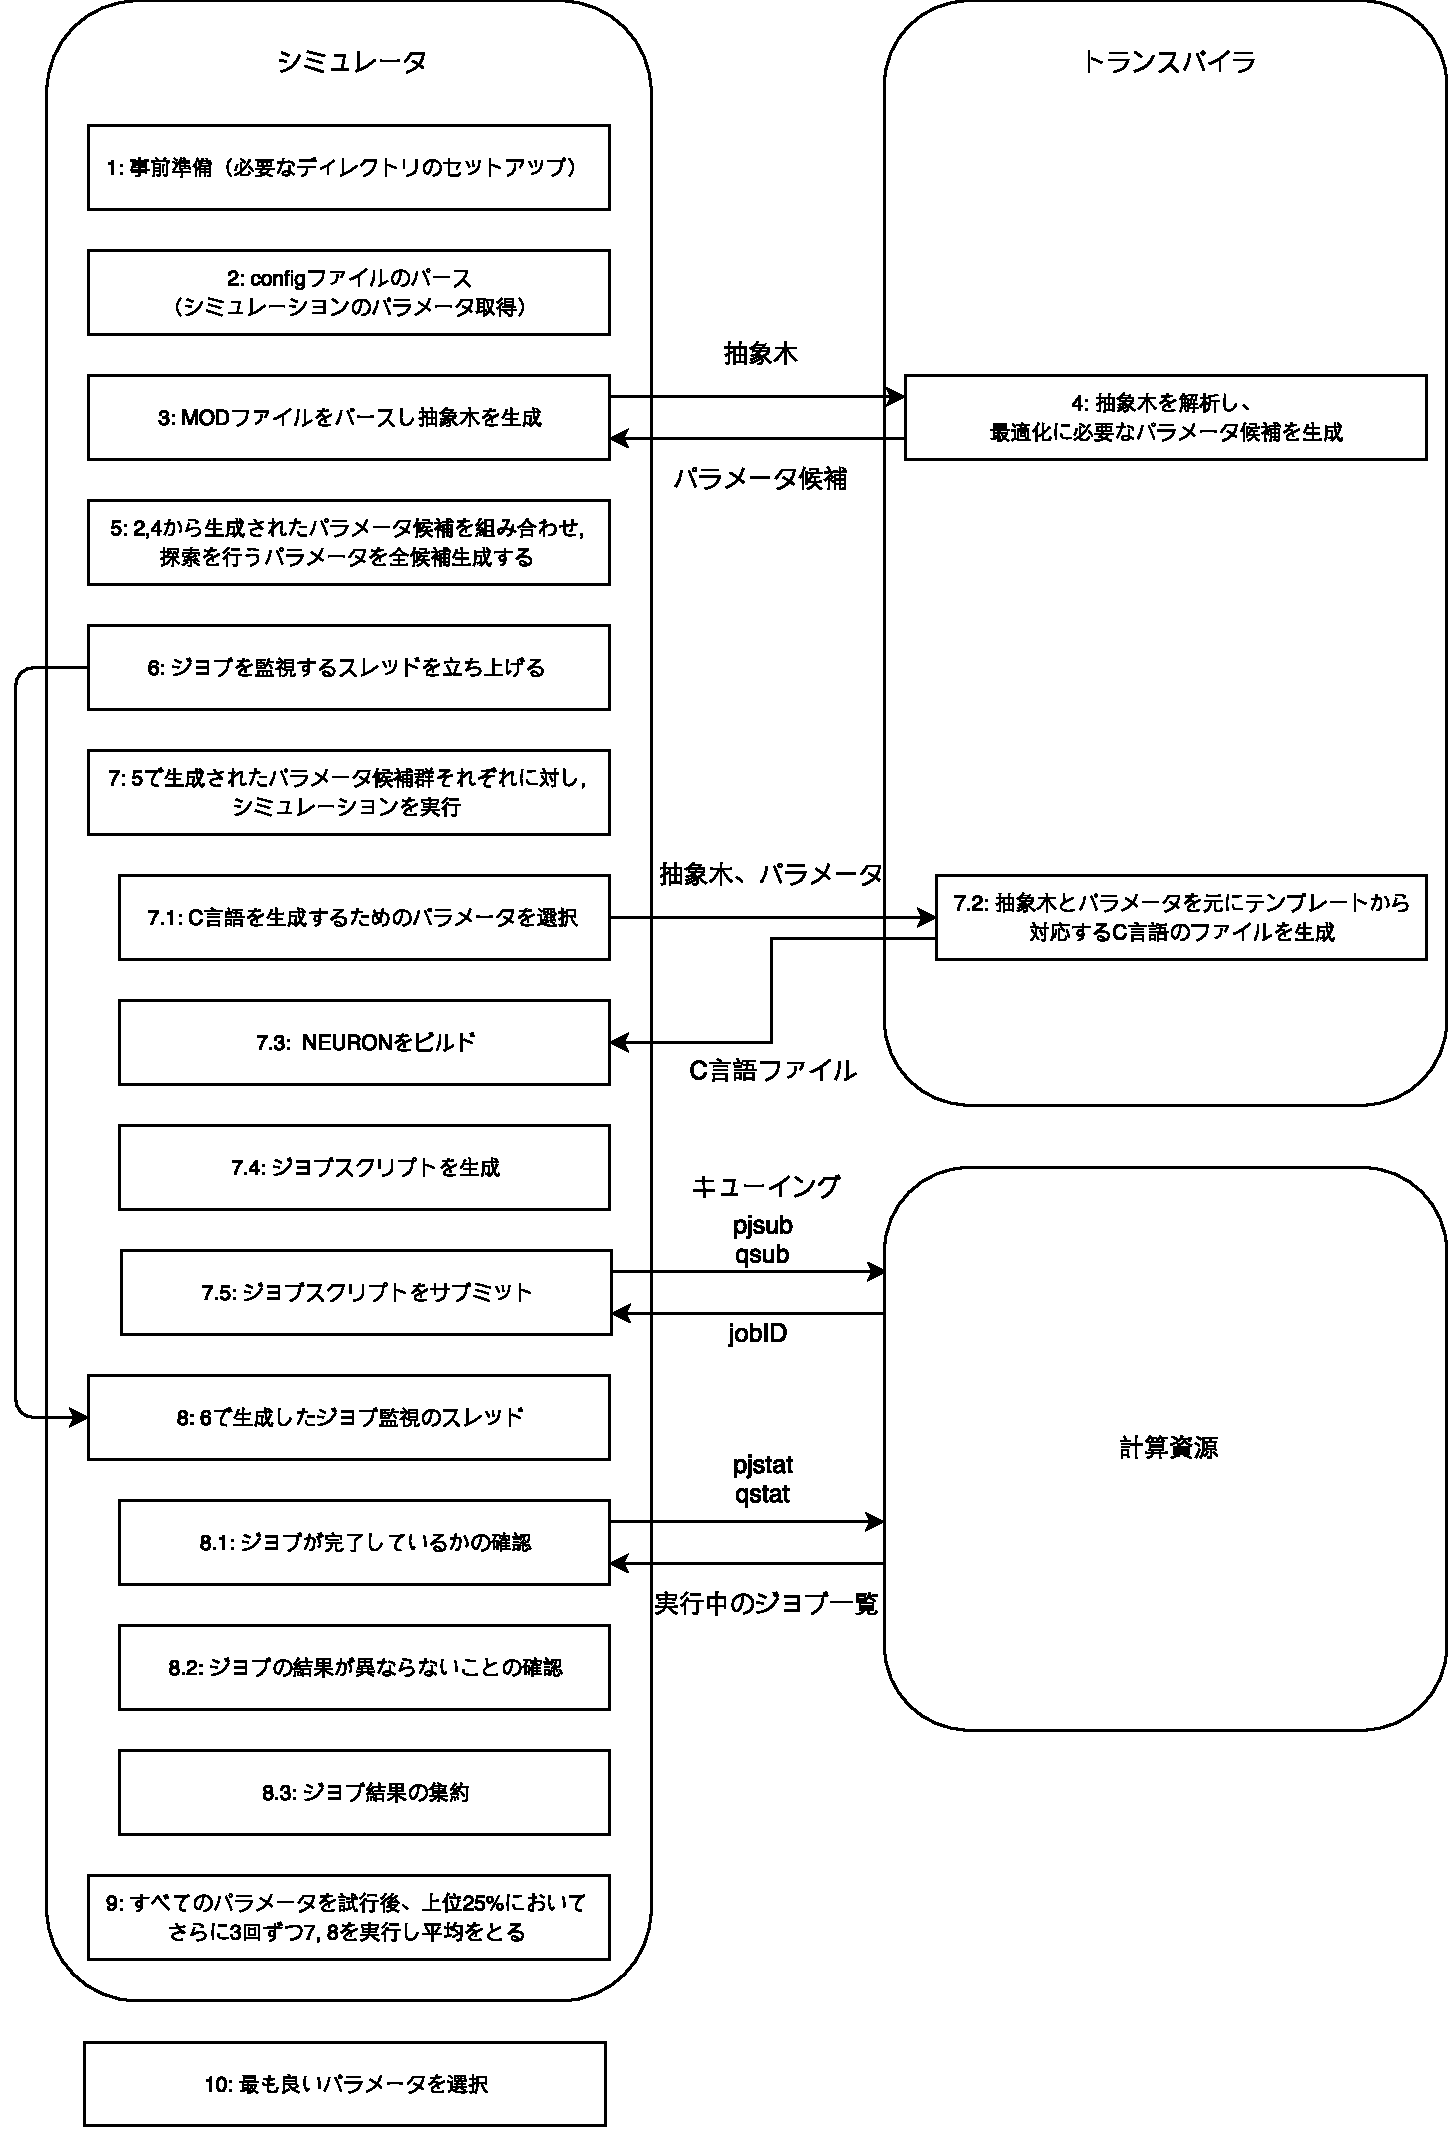
\includegraphics[width=18.0cm]{./images/Genie.pdf}
    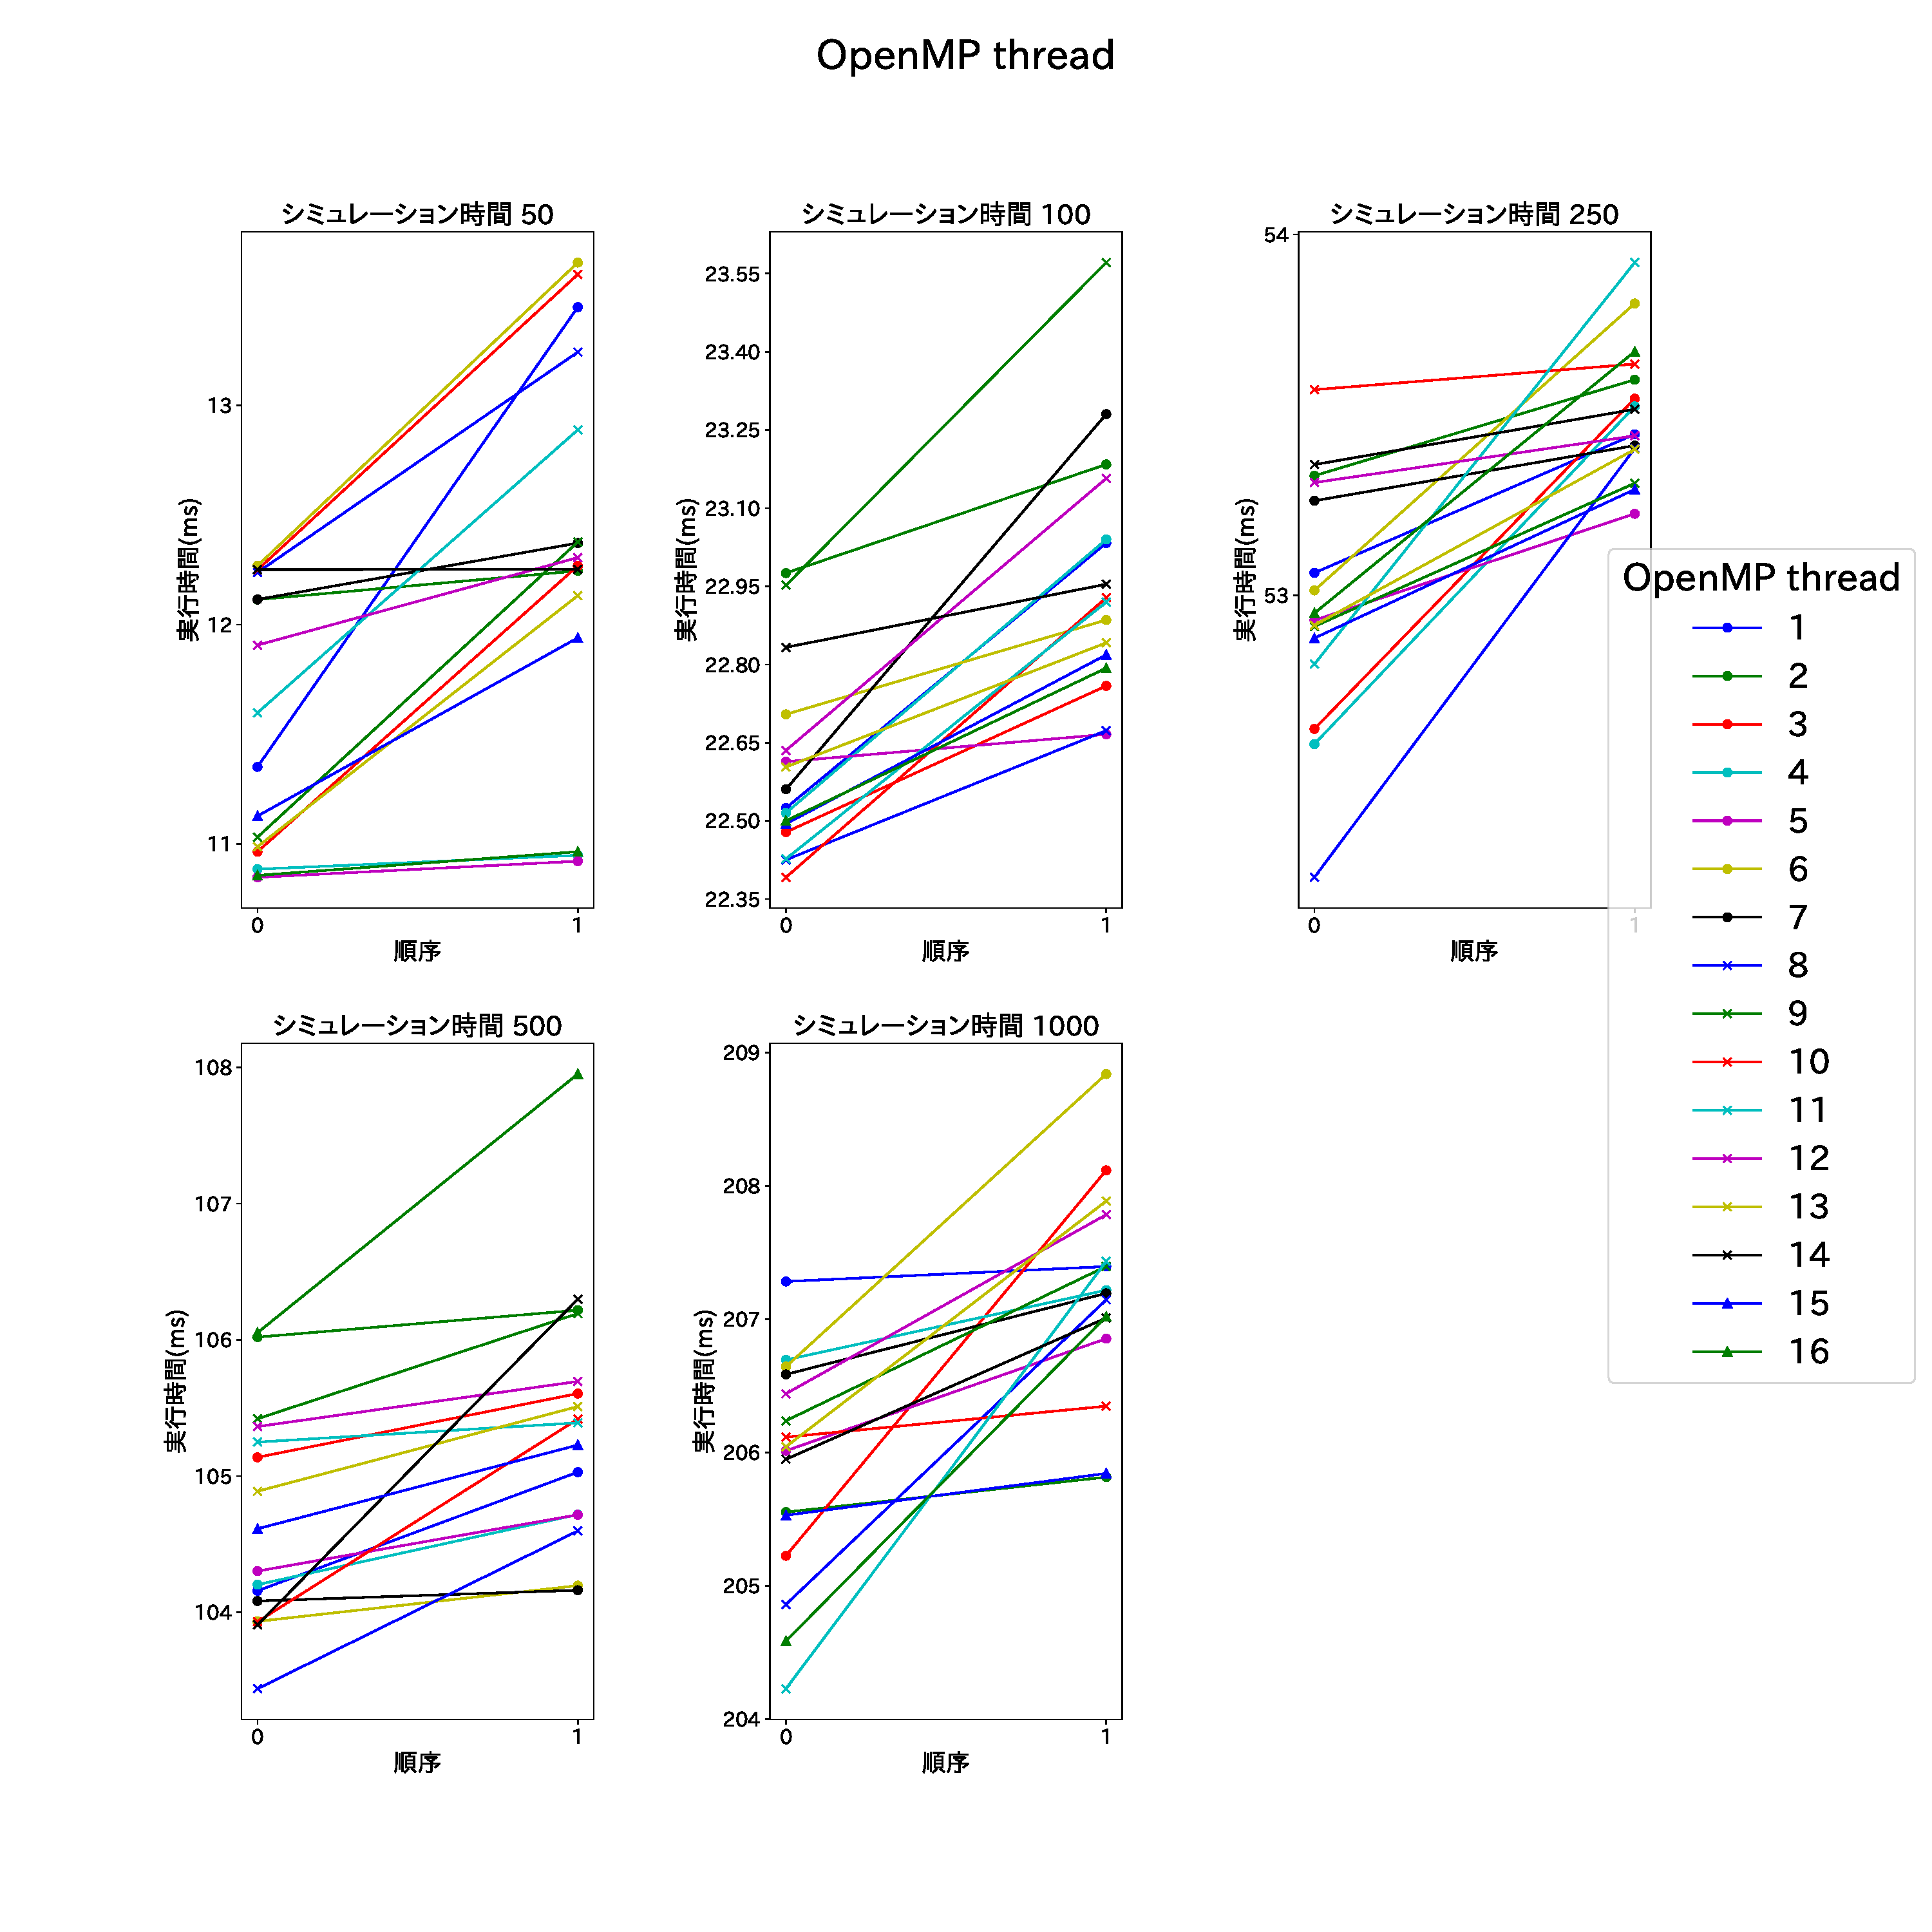
\includegraphics[width=14cm]{./images/k-OpenMP-thread.pdf}
    \caption{京 OpenMPスレッド数 シミュレーション結果}
    \label{fig:k-openmp}
\end{center}
\end{figure}
\clearpage
\subsubsection{配列のくくり出し}
\paragraph{クラスタ}~\\
 変数の配列化を通してコンパイラによるSIMD化を促進することで計算能力が大きく向上することは,
前節の結果から読み取れる. ここでは配列化を行った変数に対してさらにくくり出しを行った場合と行わなかった場合を比較する.\\
 また図\ref{fig:cluster-roa}において実行時間が早い前半部分が潰れてしまっているため,
図\ref{fig:cluster-roa-top50}に他のパラメータと同じく拡大した図を示す.\\
\begin{figure}[htb]
% h:here, t:top, b:bottom, p:page
\begin{center}
%    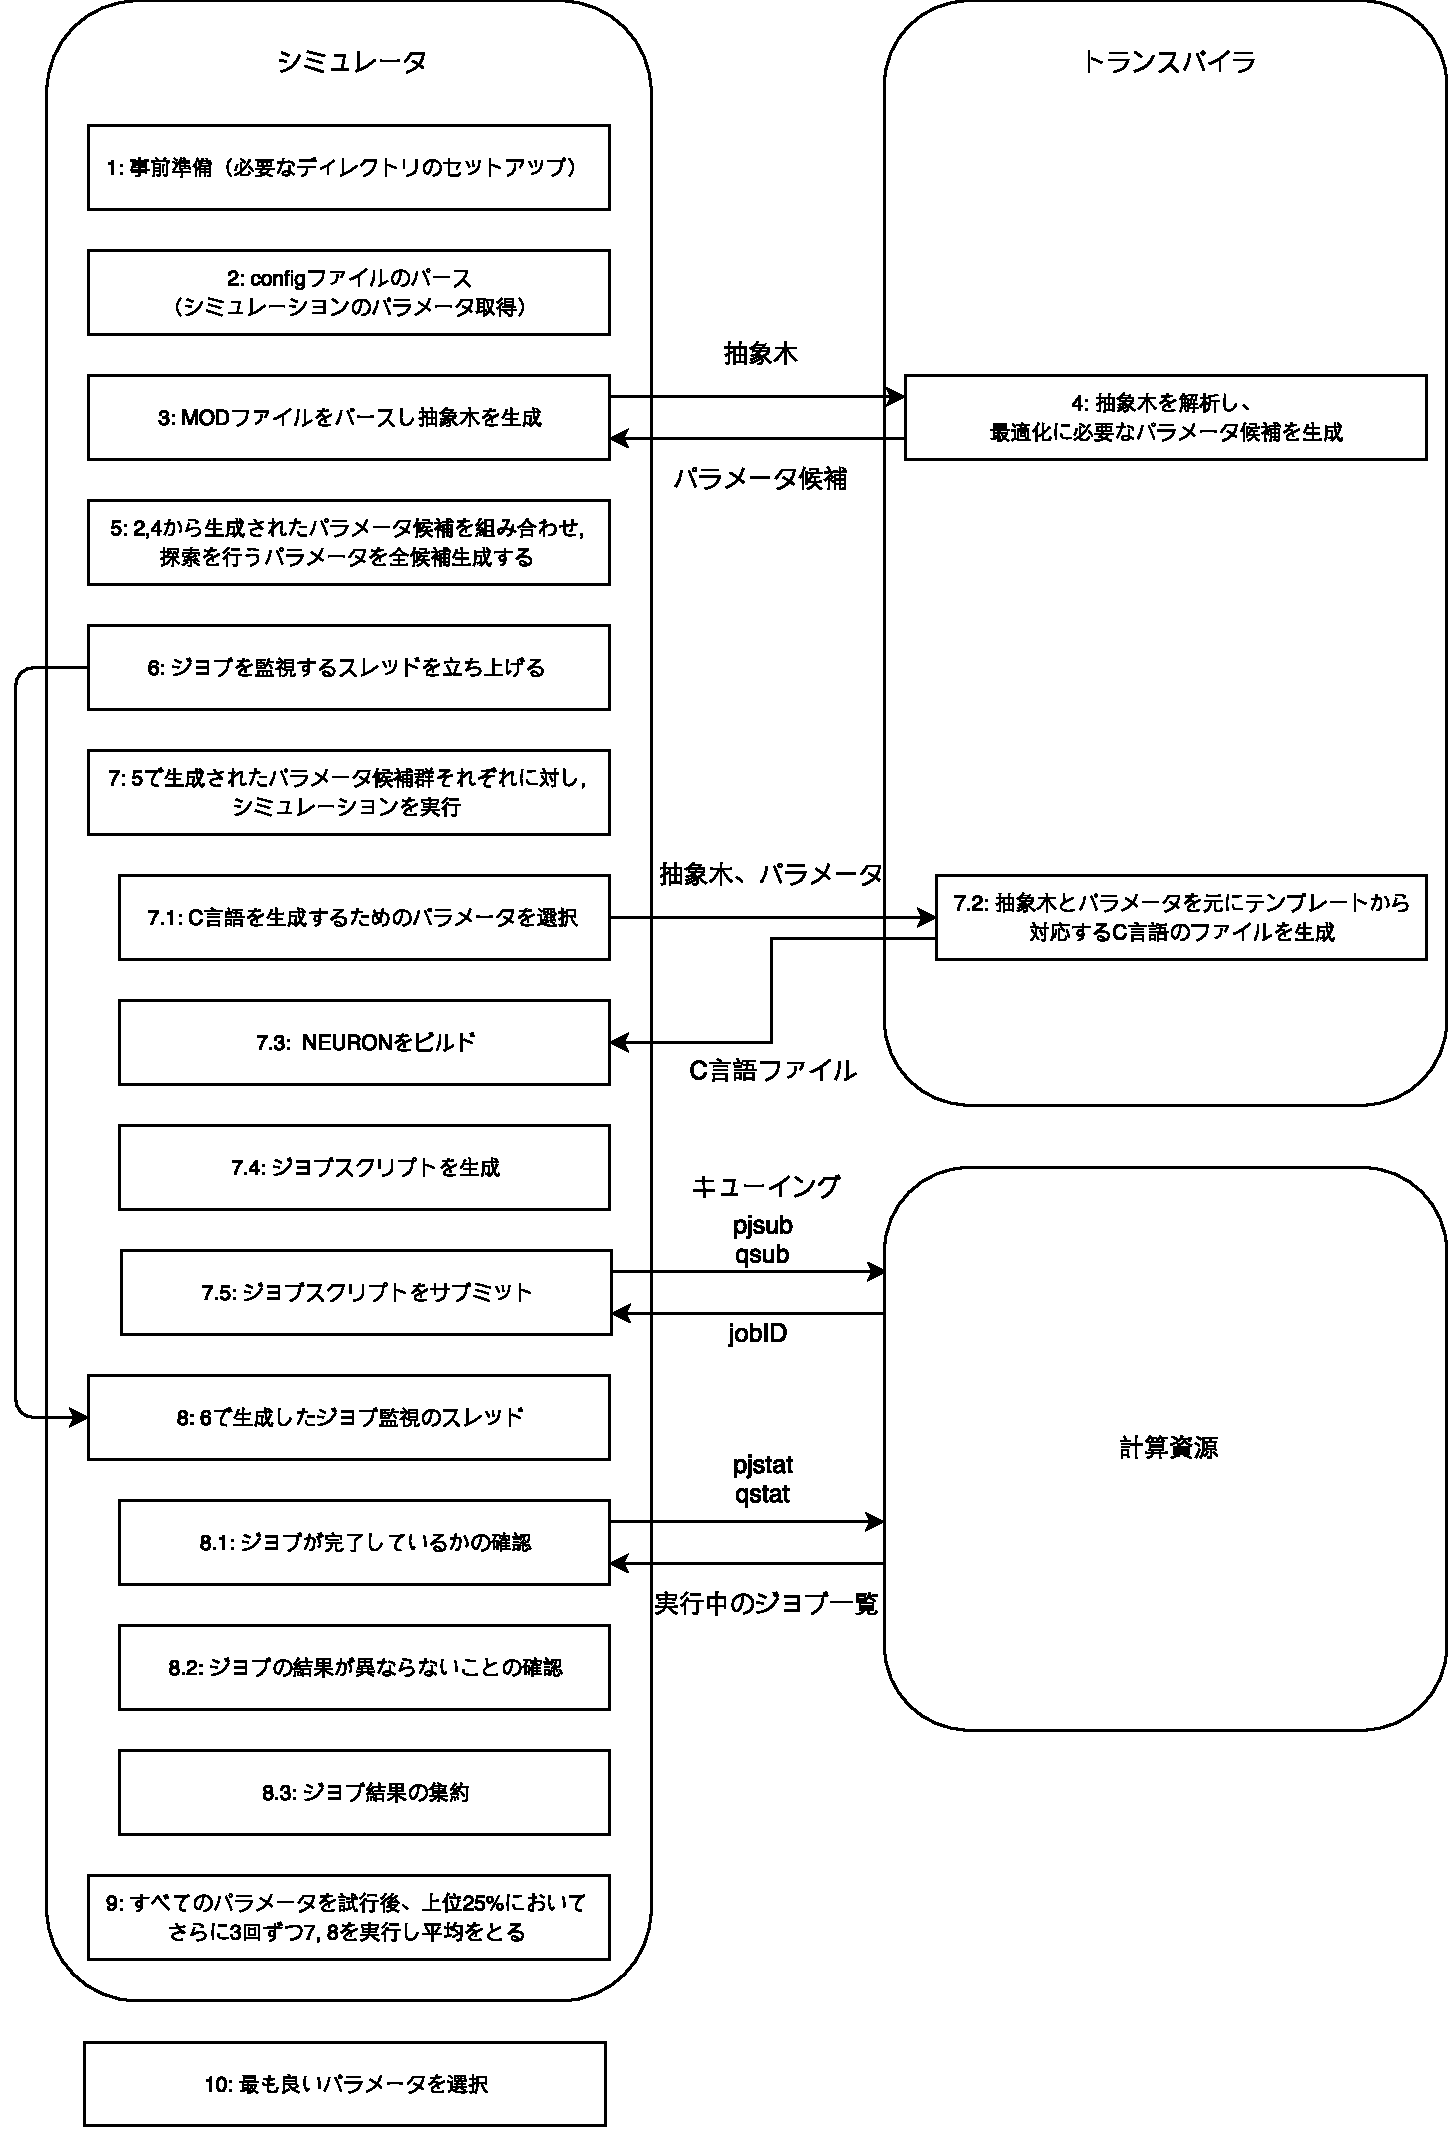
\includegraphics[width=18.0cm]{./images/Genie.pdf}
    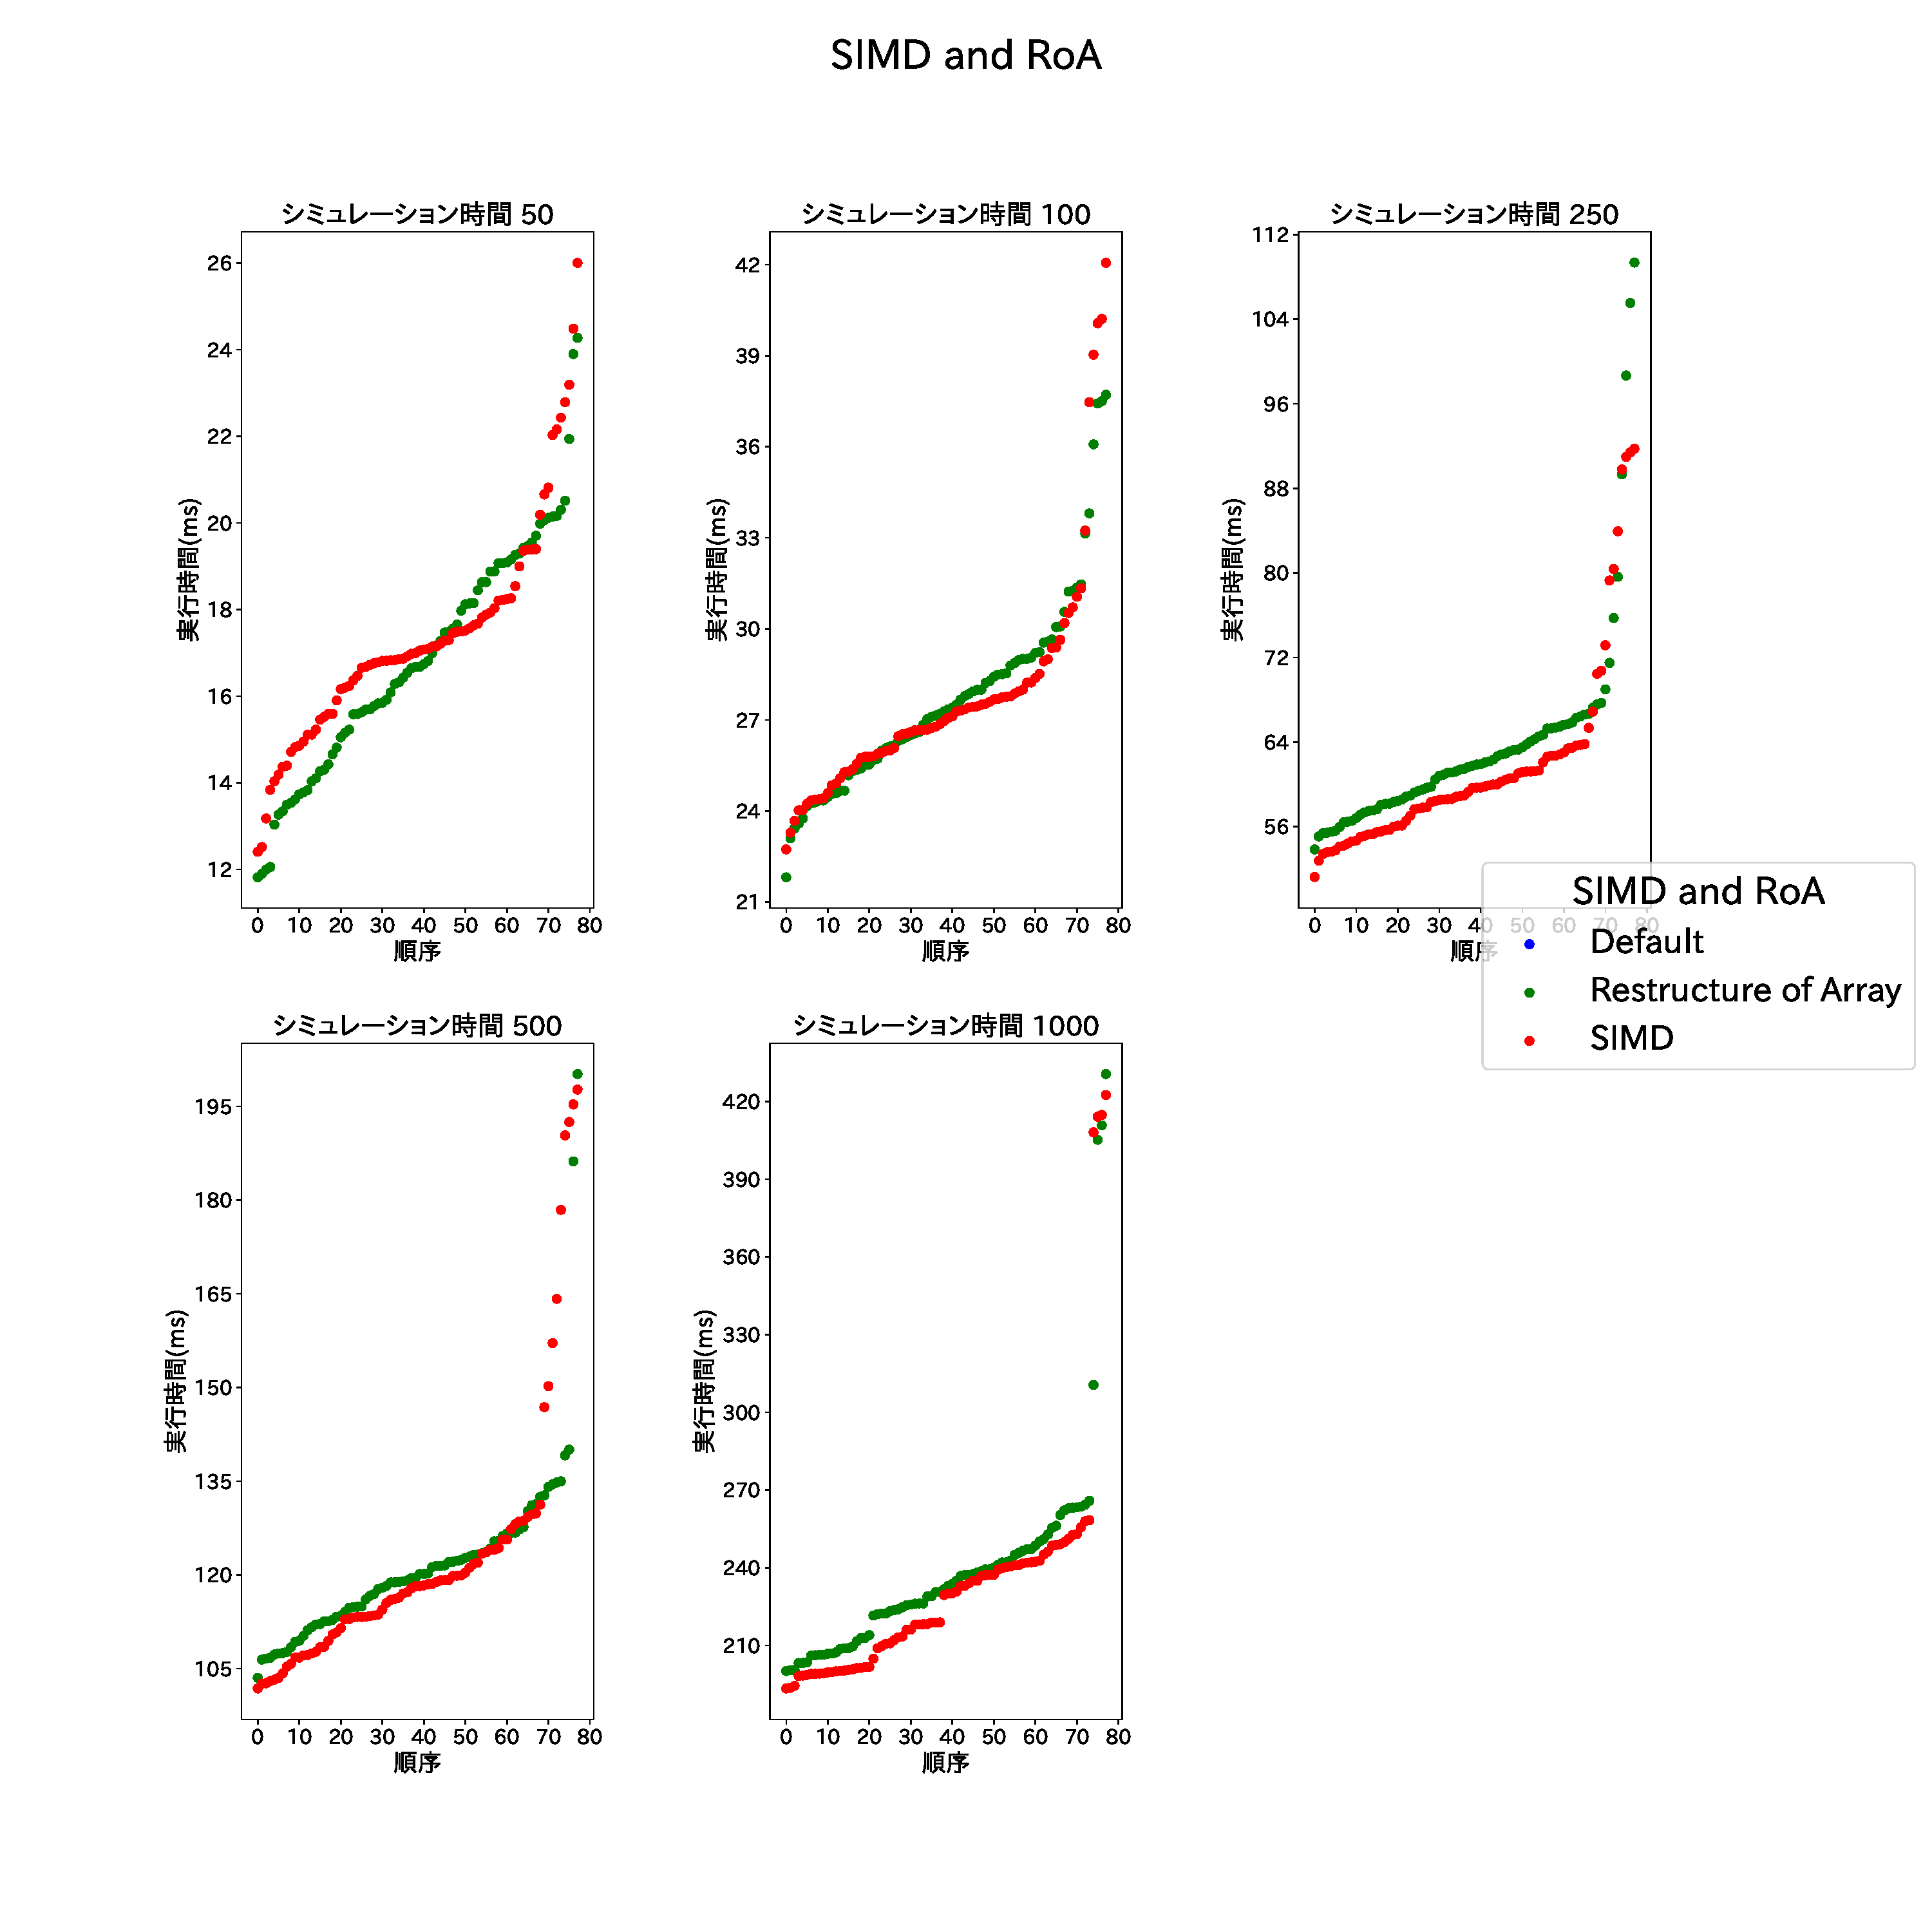
\includegraphics[width=14cm]{./images/cluster-SIMD-and-RoA.pdf}
    \caption{クラスタ 配列のくくり出し シミュレーション結果}
    \label{fig:cluster-roa}
\end{center}
\end{figure}

\begin{figure}[htb]
% h:here, t:top, b:bottom, p:page
\begin{center}
%    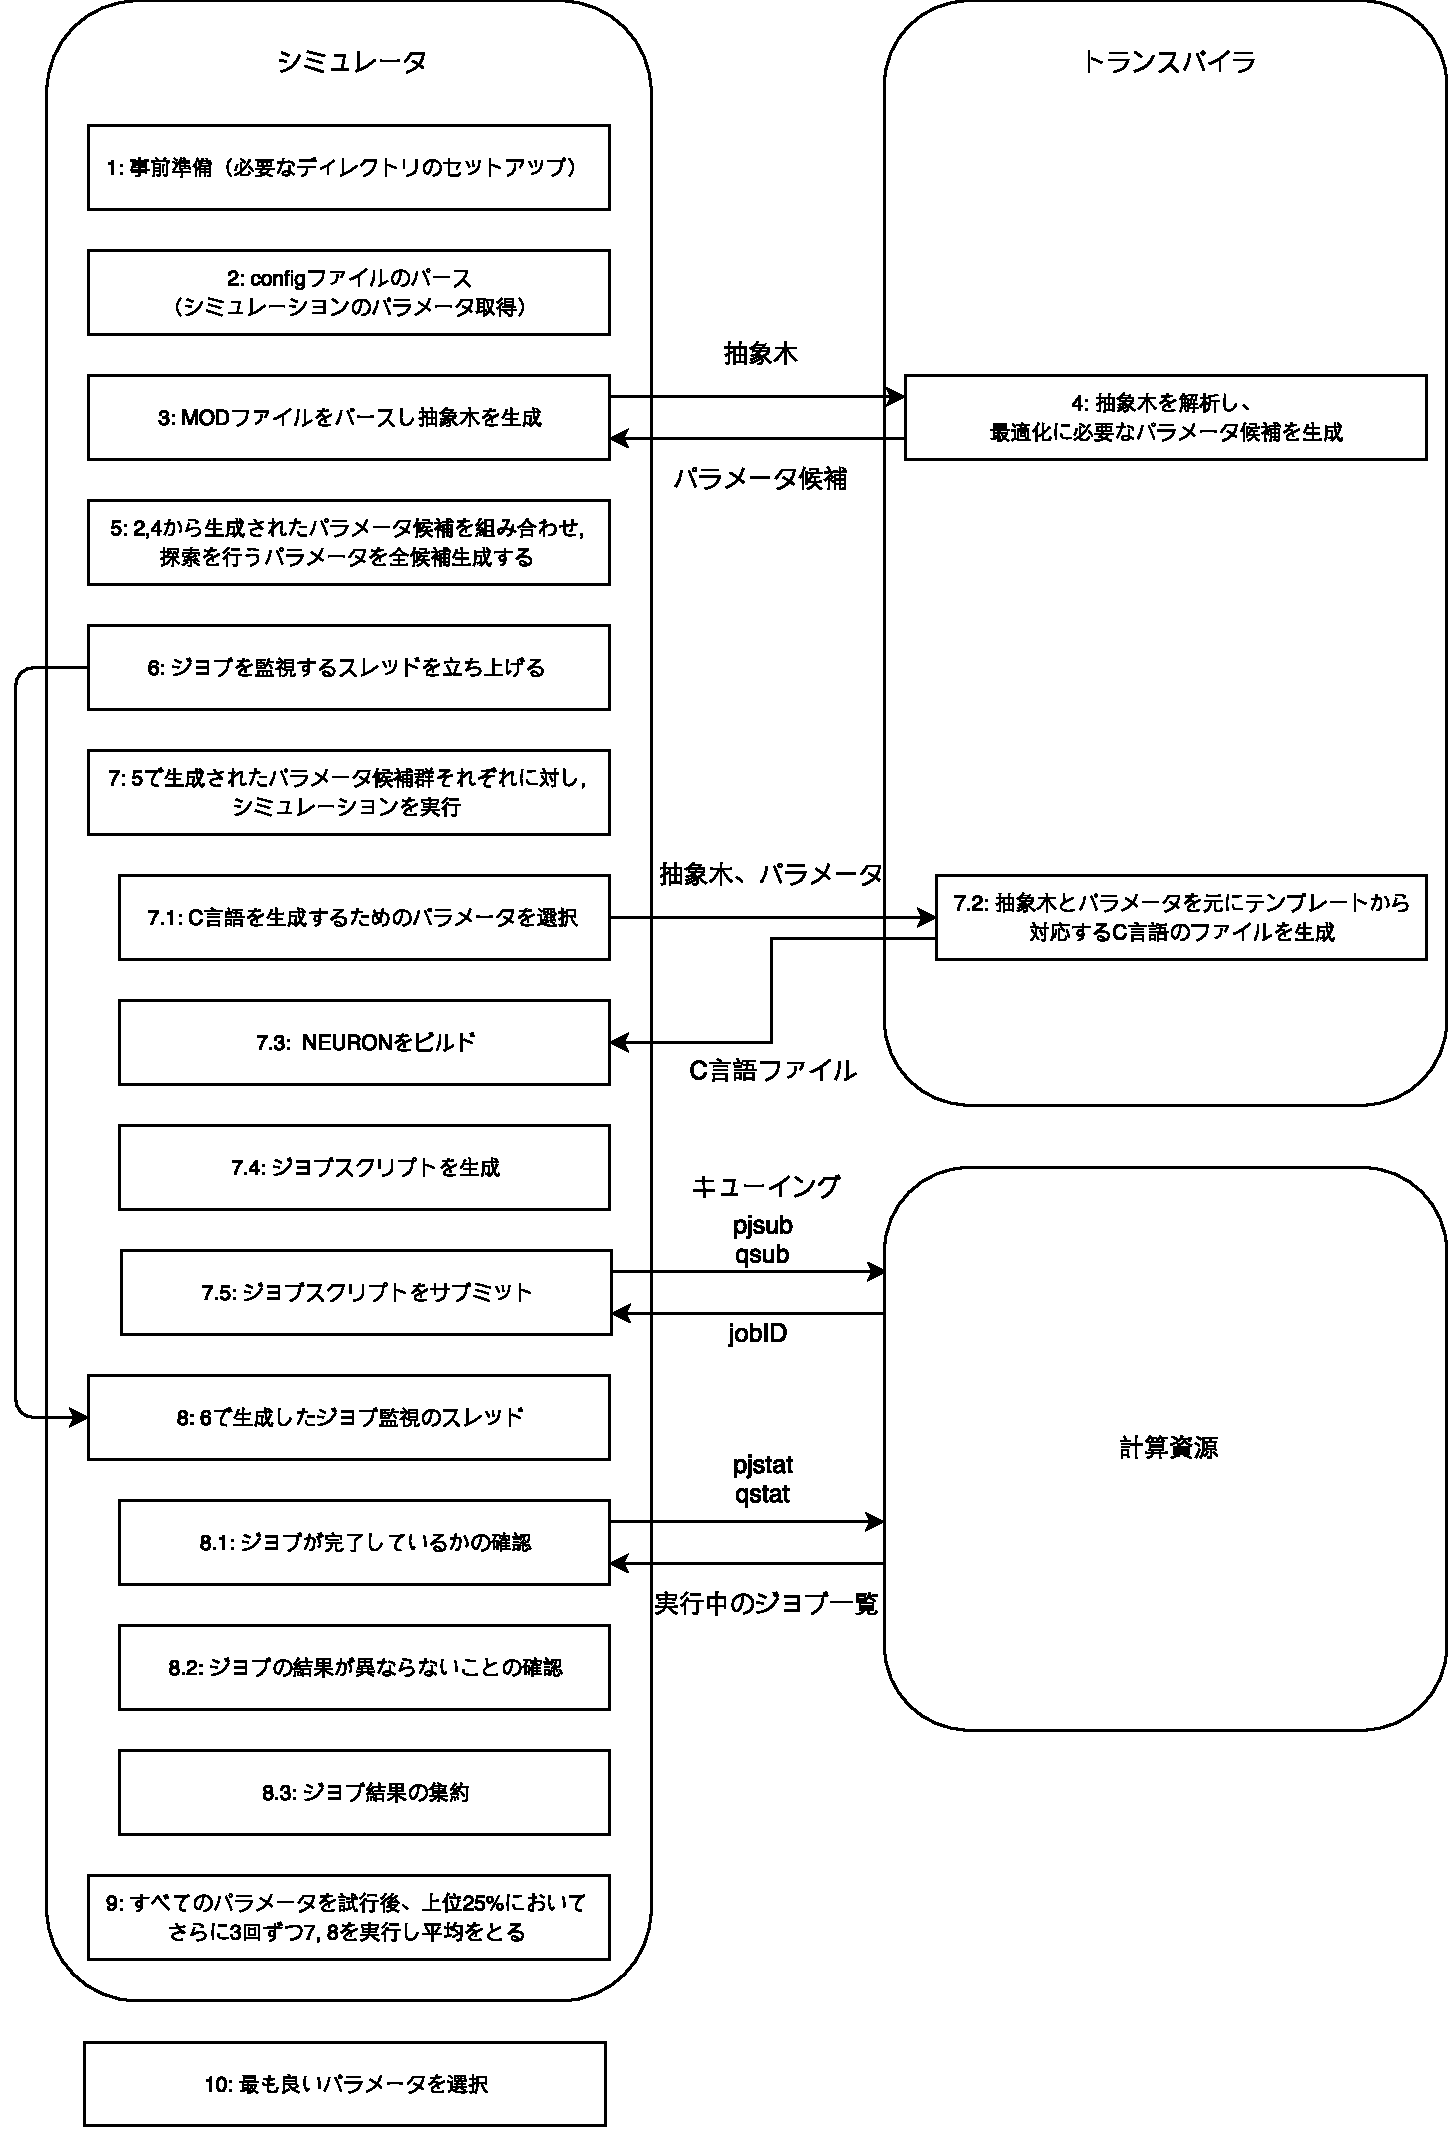
\includegraphics[width=18.0cm]{./images/Genie.pdf}
    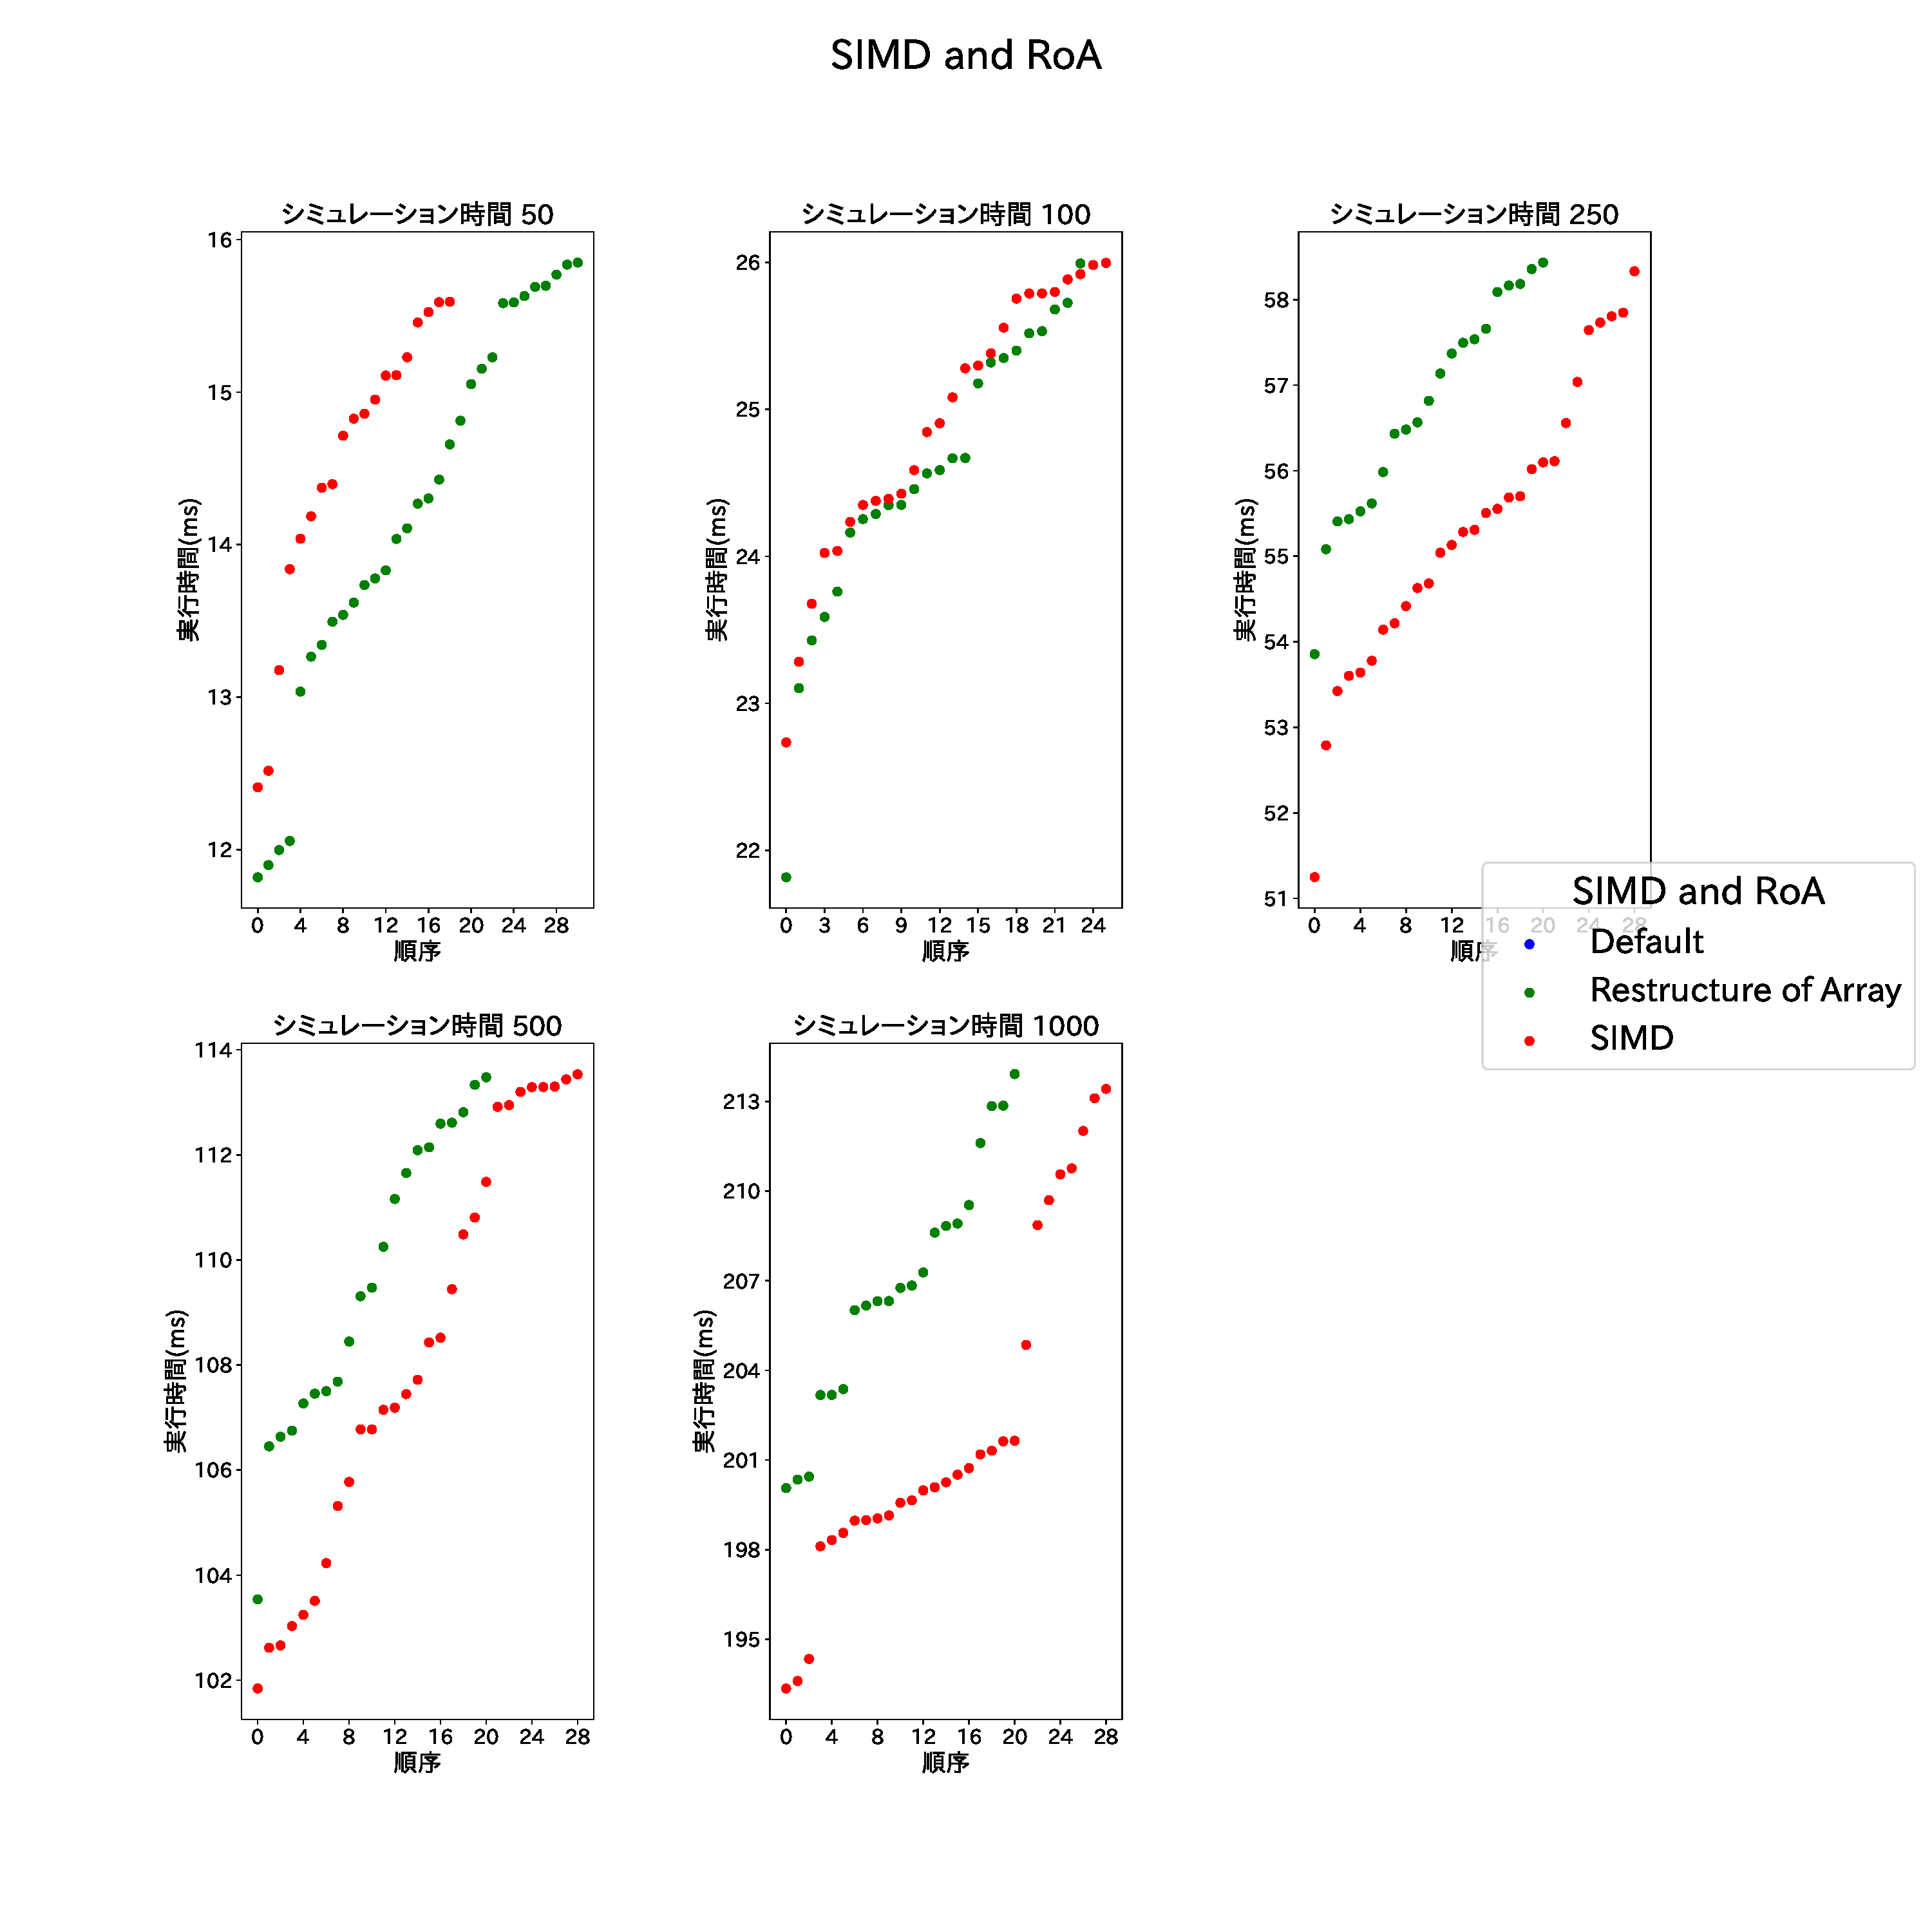
\includegraphics[width=14cm]{./images/cluster-top50-SIMD-and-RoA.pdf}
    \caption{クラスタ 配列のくくり出し シミュレーション結果 上位50組}
    \label{fig:cluster-roa-top50}
\end{center}
\end{figure}

シミュレーション時間が長くなるに連れ,
配列のくくり出しを行わずSIMD化のみを用いたほうが高速化されるように見られるが,
実行時間の差を比較するとシミュレーション時間が倍になった場合でもほぼ一定の差になっているため,
本論文執筆時においての実装では実行時間への影響は少ないことがわかる.\\

\paragraph{京}~\\
 一方で, 京環境においてはクラスタ環境と比べ図\ref{fig:k-roa}にあるように,
配列のくくり出しを行う場合と行わない場合で実行時間の差はより小さくなっている.\\
 このことから京環境においてはデフォルトのコンパイラの性能がGCCと比べて高く,
くくり出しの有無にかかわらず十分な最適化がなさているのではないかと考えられる.\\
\begin{figure}[htb]
% h:here, t:top, b:bottom, p:page
\begin{center}
%    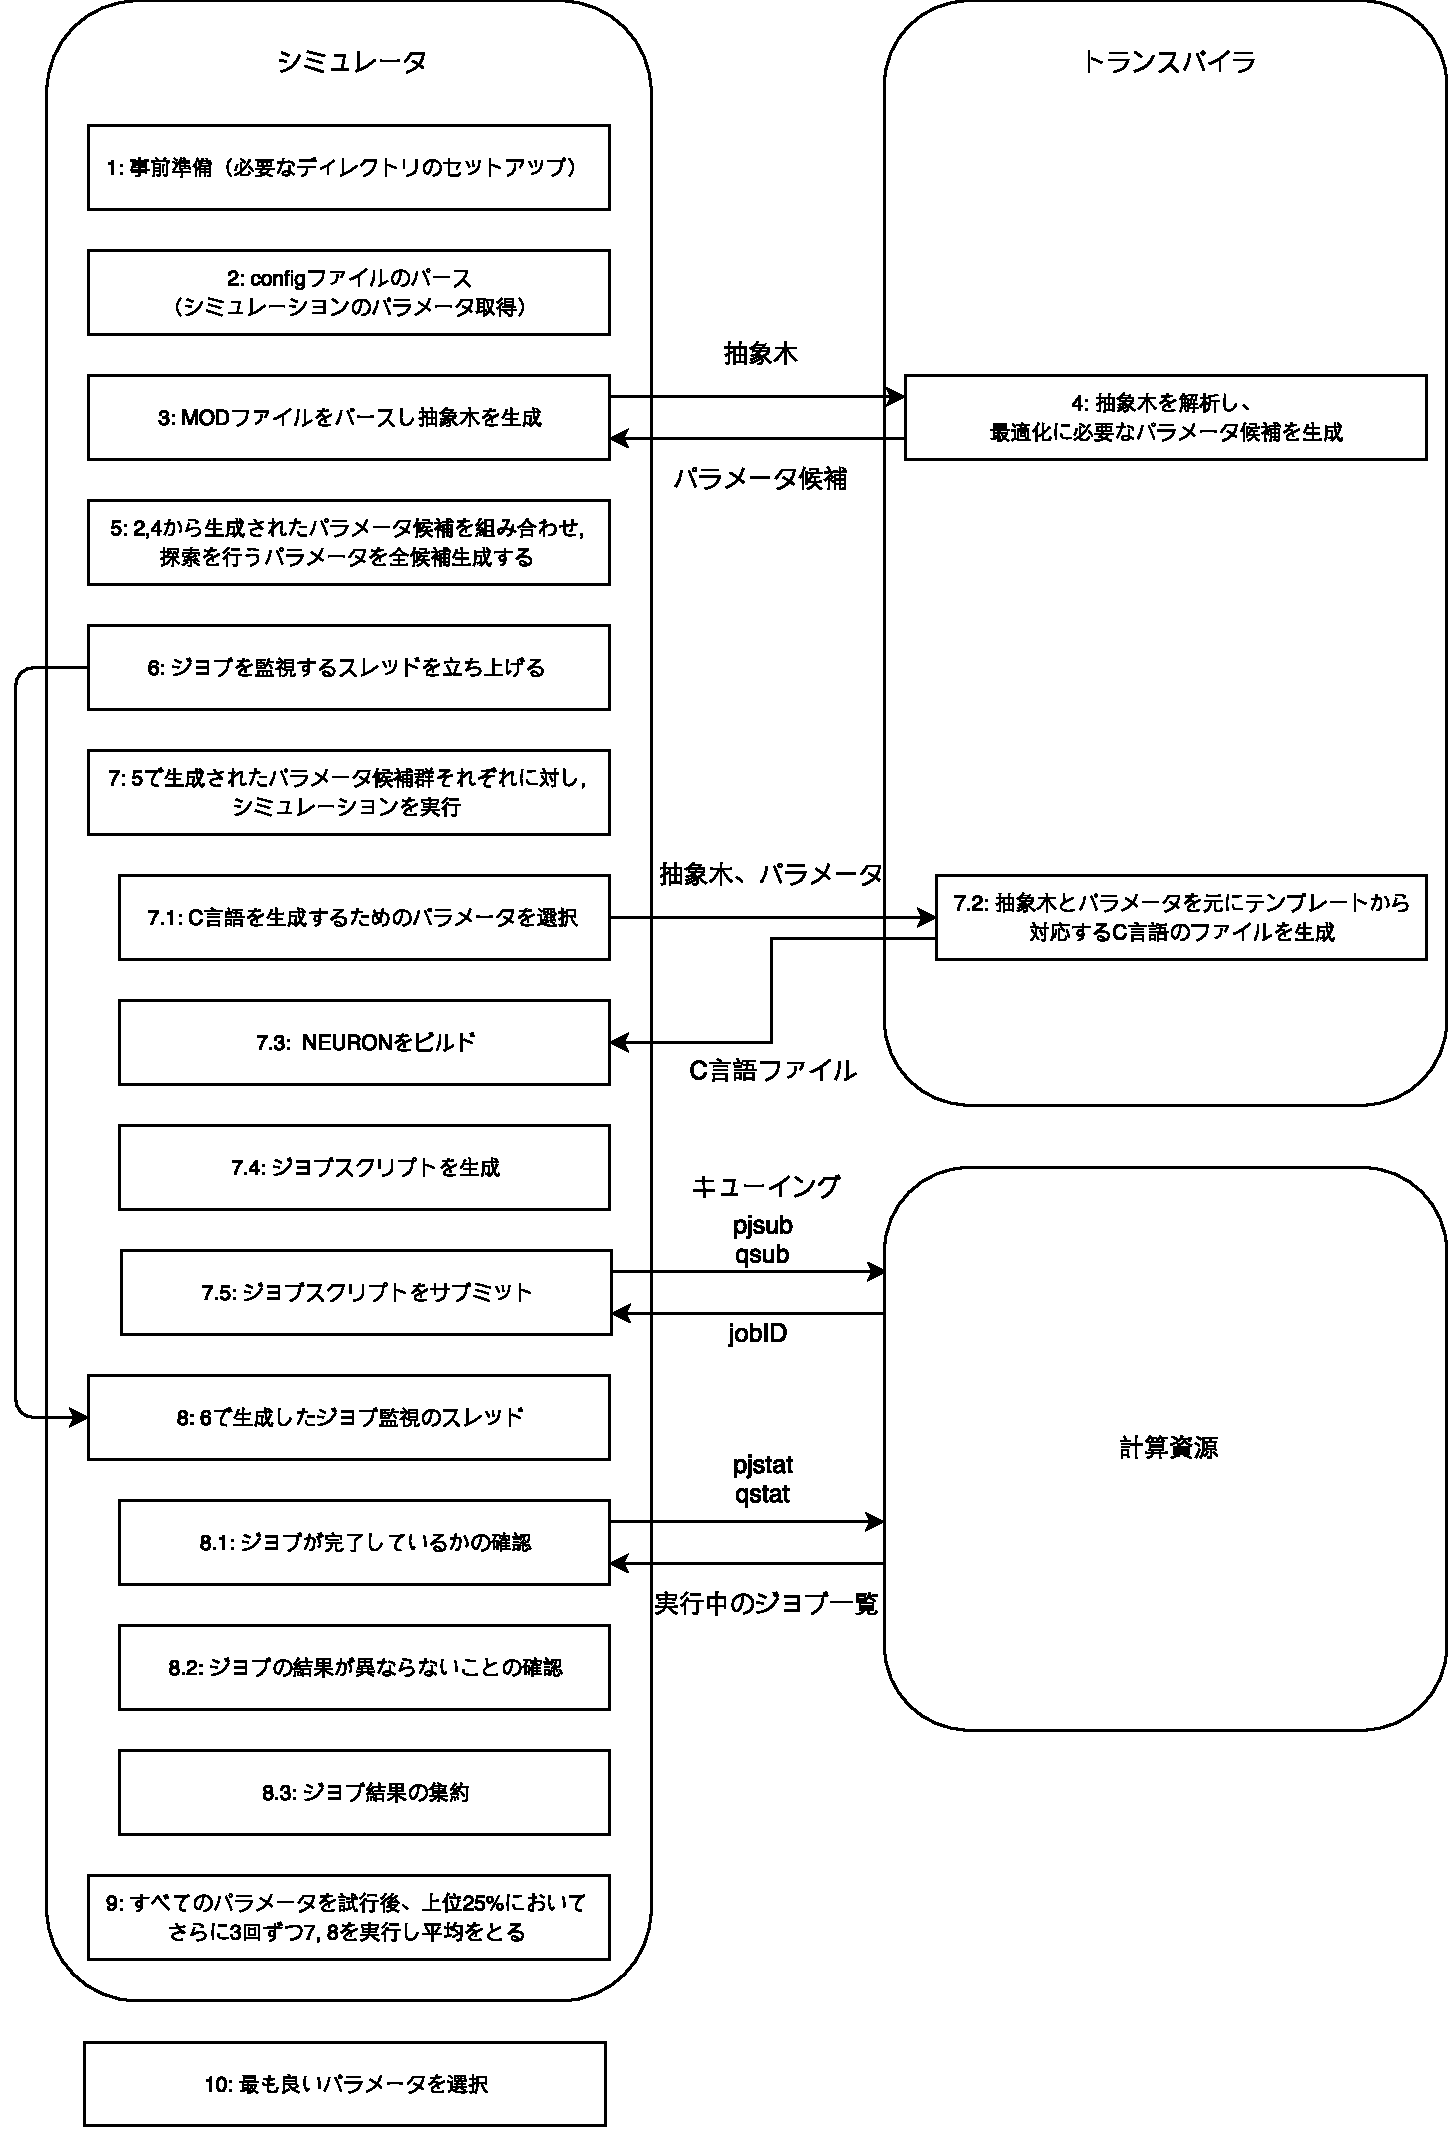
\includegraphics[width=18.0cm]{./images/Genie.pdf}
    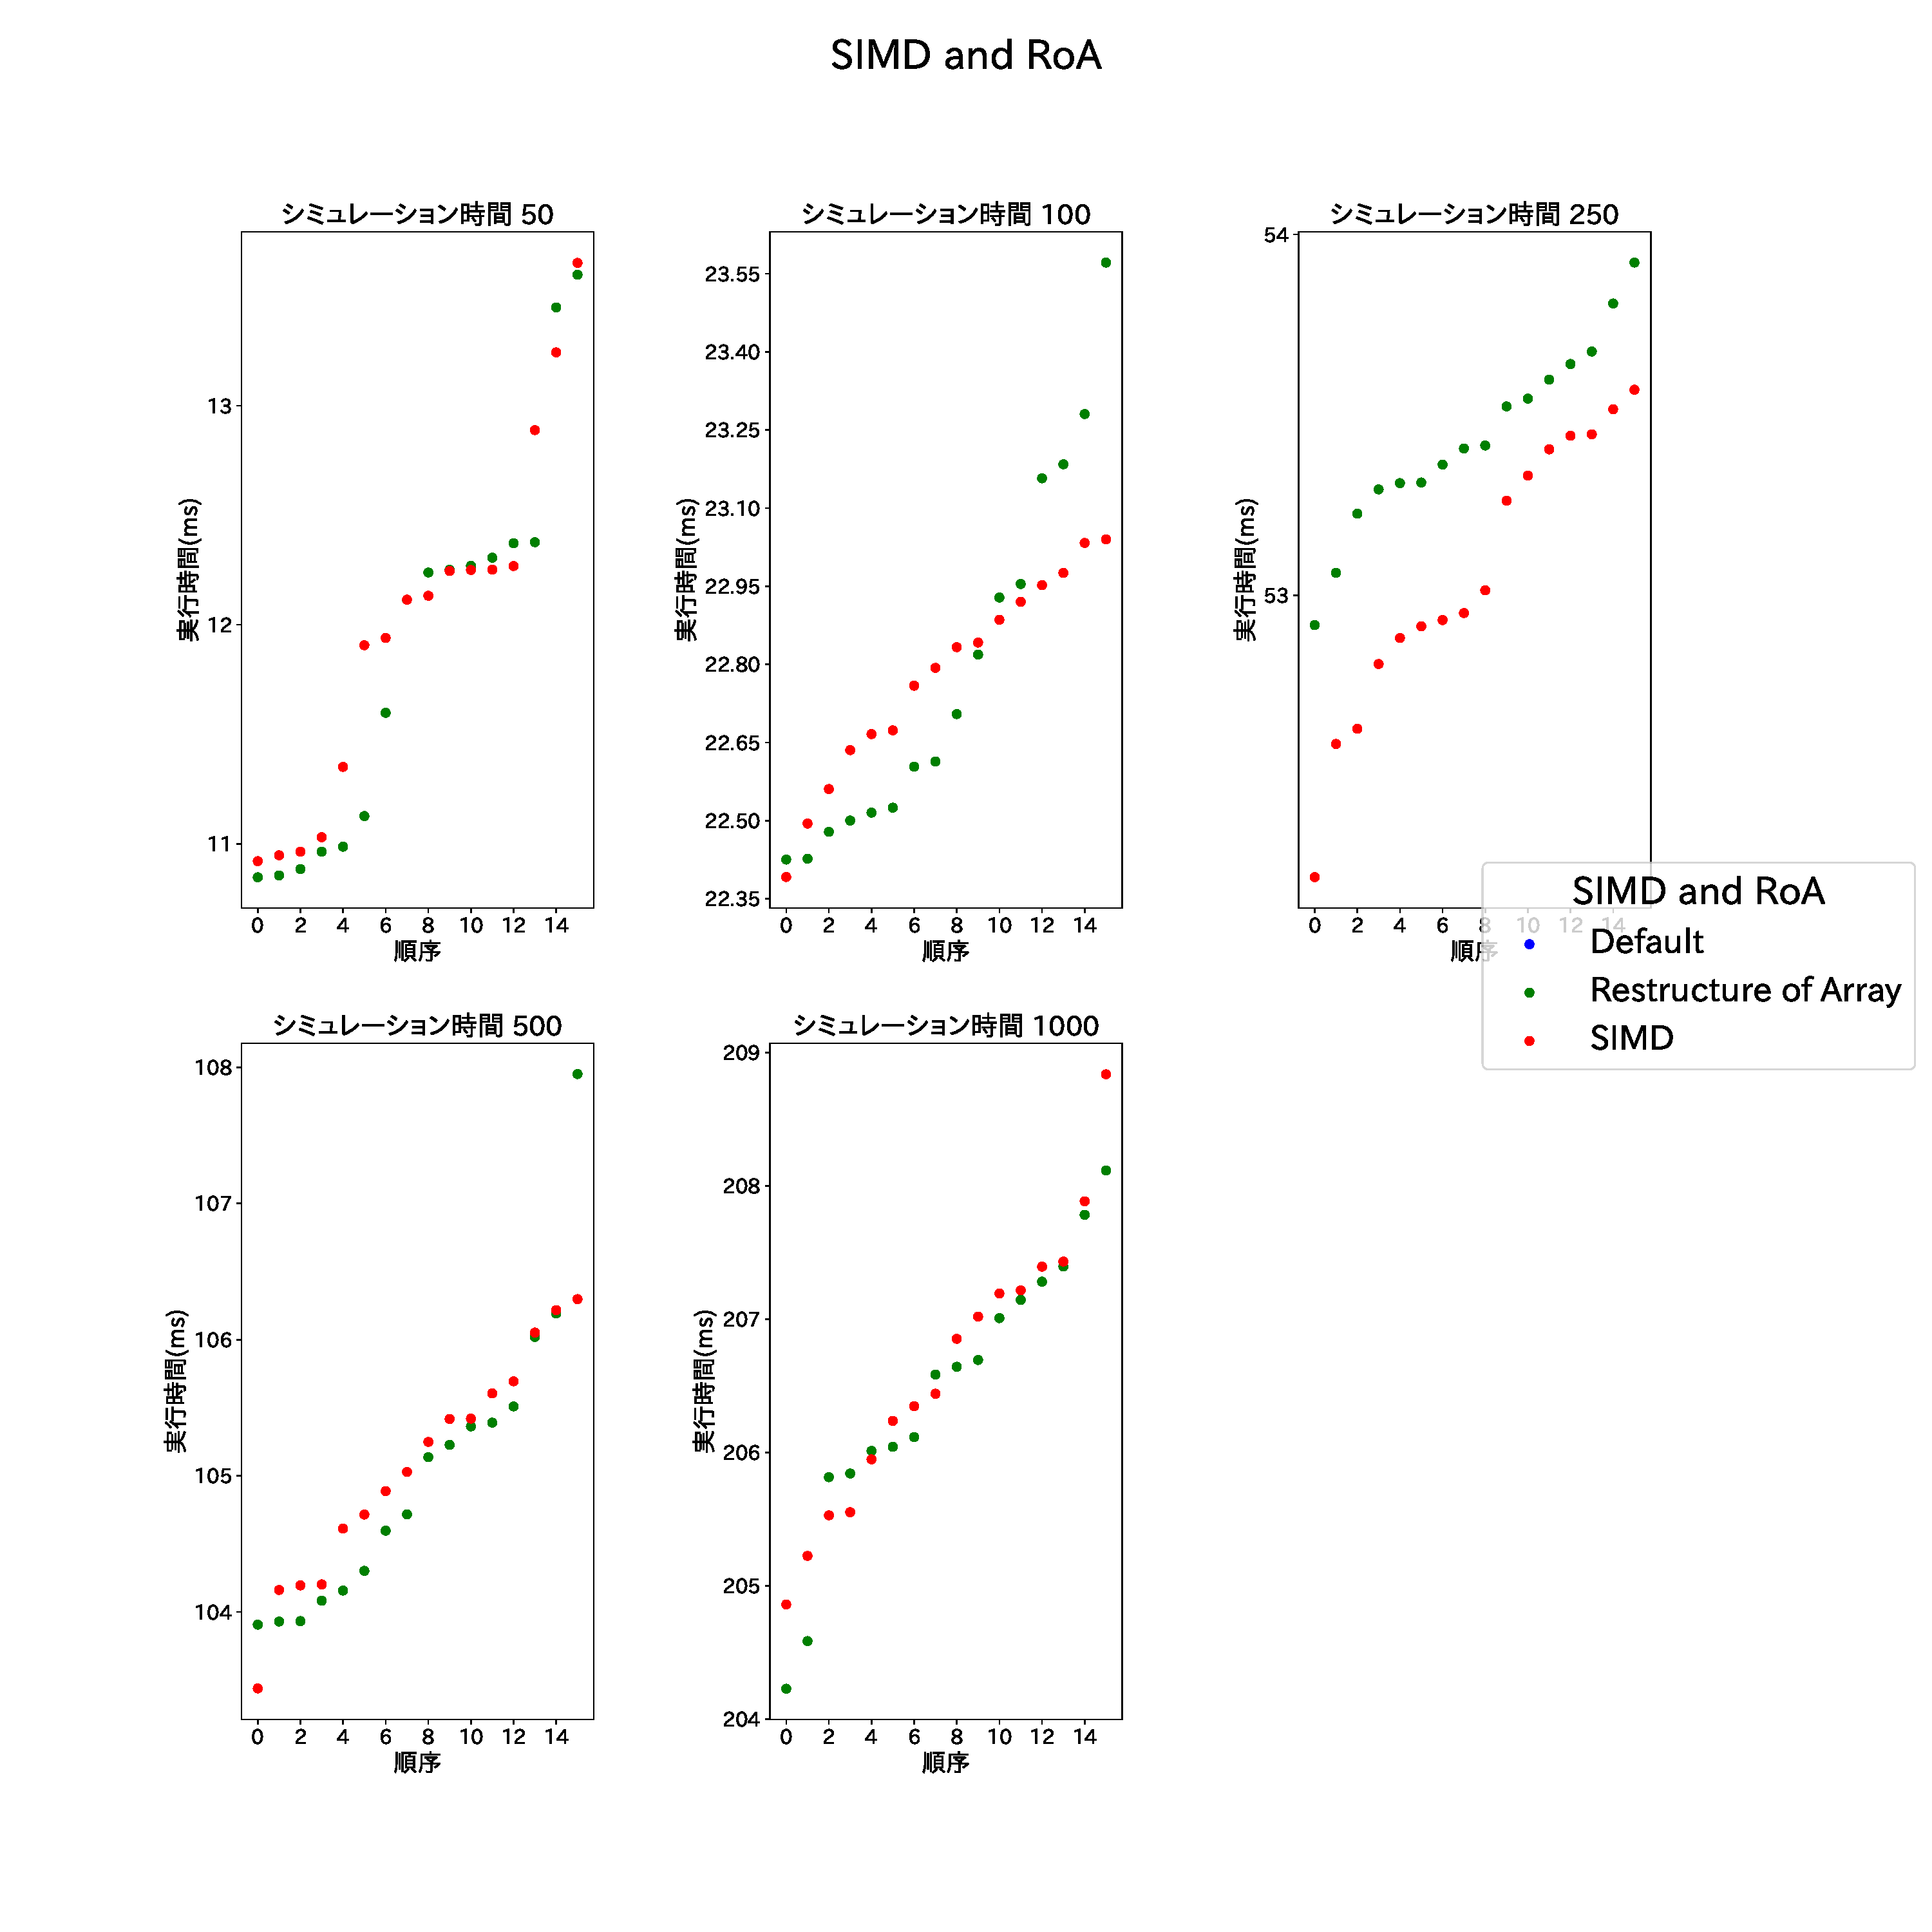
\includegraphics[width=14cm]{./images/k-SIMD-and-RoA.pdf}
    \caption{京 配列のくくり出し シミュレーション結果}
    \label{fig:k-roa}
\end{center}
\end{figure}
\clearpage

\subsection{自動最適化の評価}
\label{subsec:compare}
最後に, \ref{subsec:small-sim}節を通して求めたシミュレーションの実行時間が最も短くなるパラメータを用いて表\ref{table:sim-cond}に示した条件のシミュレーションを行い,
他の方法で最適化を行った結果と比較することで自動最適化の効果を定量的に評価する.\\
\begin{table}[htb]
\caption {自動最適化の評価 シミュレーション条件}
\begin{center}
  \begin{tabular}{|p{6cm}|p{8cm}|}
    \hline
    パラメータ & 値の範囲\\ \hline
    シミュレーション時間 & 1000\\ \hline
    神経細胞数 & 256\\ \hline
    ネットワーク & Watts and Strogatzネットワーク\\ \hline
    試行回数 & 10回 \\ \hline
  \end{tabular}
  \label{table:sim-cond}
\end{center}
\end{table}

また自動最適化の結果として用いたパラメータは,
\ref{subsec:detail-sim}節においてシミュレーション時間1000msで行ったシミュレーションの内,
平均の実行時間がもっとも短いパラメータの組を用いる.\\
\begin{table}[htb]
  \caption {自動最適化パラメータ}
  \begin{center}
    \begin{tabular}{|p{4cm}|p{5cm}|p{5cm}|}
      \hline
      パラメータ & クラスタでの値 & 京での値\\ \hline
      MPIプロセス数 & 26 & 8\\ \hline
      OpenMPスレッド数 & 2 & 11\\ \hline
      SIMD化 & 行う & 行う\\ \hline
      配列のくくり出し & 行わない & 行う \\ \hline
    \end{tabular}
    \label{table:auto-tuned-param}
  \end{center}
\end{table}\\

シミュレーションを行う上で, 比較対象として用いたものを次に示す.
\begin{itemize}
\item 自動最適化を行ったNEURON
\item デフォルトの状態のNEURON
\item MPIプロセス数とOpenMPスレッド数の最適化結果を用いたNEURON
\item ICCを用いてコンパイルを行ったNEURON(クラスタのみ)
\item 手動での最適化を行ったNEURON(先行研究\cite{miyamoto-master}を利用)
\end{itemize}
 尚, デフォルトの状態はMPIプロセス数がCPUの数(クラスタでは2, 京では1)であり,
OpenMPスレッド数は各CPUのコア数(クラスタでは14, 京では8)として定義した.
\subsubsection{クラスタ}~\\
 10回のシミュレーションを行う上で, 平均だけでなく各シミュレーションごとの誤差を見るため,
図\ref{fig:cluster-compare}に示すように箱ひげ図を用いてグラフ化した.\\
 図\ref{fig:cluster-compare}において, デフォルトの設定は実行時間に幅はあるものの多くの場合5000sを超える実行時間がかかっていることがわかる.\\
\begin{figure}[htb]
% h:here, t:top, b:bottom, p:page
 \begin{center}
    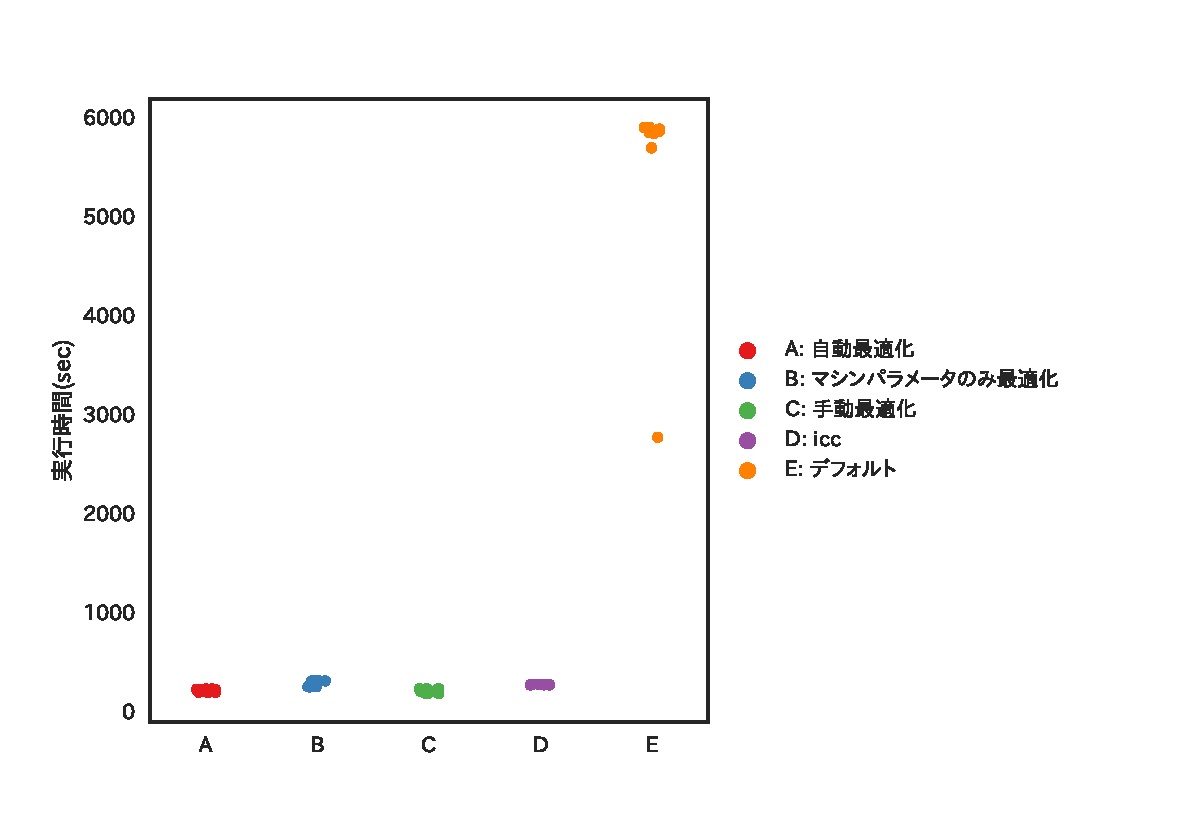
\includegraphics[width=14cm]{./images/cluster-compare.pdf}
    \caption{クラスタ 自動最適化評価}
    \label{fig:cluster-compare}
  \end{center}
\end{figure}~\\
 次にデフォルトを除いた他の4つの条件のみを図\ref{fig:cluster-compare-2}に示す.\\
\begin{figure}[htb]
% h:here, t:top, b:bottom, p:page
 \begin{center}
    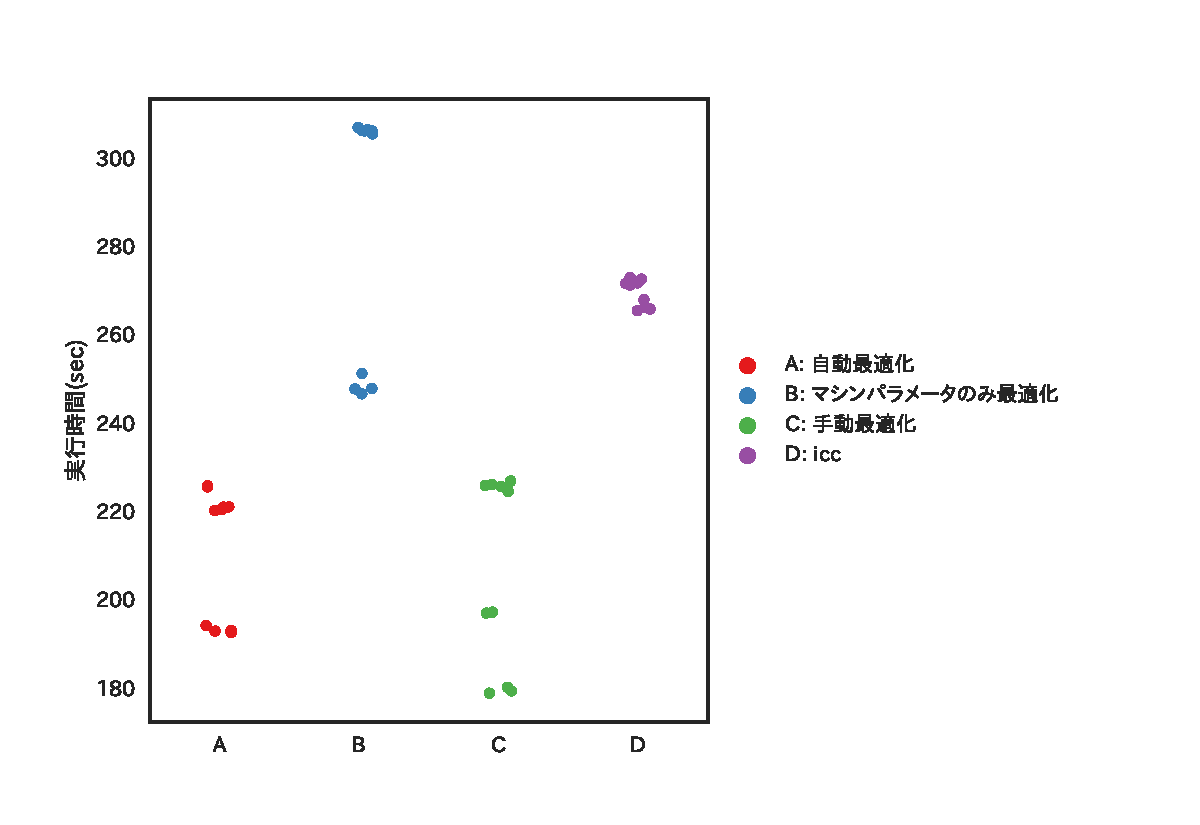
\includegraphics[width=14cm]{./images/cluster-compare-2.pdf}
    \caption{クラスタ 自動最適化評価 (デフォルト以外)}
    \label{fig:cluster-compare-2}
  \end{center}
\end{figure}~\\
 この図から, 自動最適化を行ったものは手動での最適化と比べ多少劣るものの,
マシンパラメータのみの最適化を行ったものや最適化に非常に優れたコンパイラであるiccを用いたもの比較しても
十分に高速化されているといえる.\\
\vspace{10cm}
\subsubsection{京}~\\
 同様にして京においての比較結果を図\ref{fig:k-compare}に示す. また, デフォルトの設定が原因となり実行速度が早いものの結果が潰れてしまっているため, デフォルトの条件を抜いたものを図\ref{fig:cluster-compare-2}に示す.\\
 この図からわかることは, クラスタの結果と比べ個々のシミュレーションの実行時間にばらつきがないことがわかる.
これは京においてログインノードと計算用のノードが分離されているため, シミュレーションが別プロセスの影響を受けにくいからであると考えられる.\\
\begin{figure}[htb]
% h:here, t:top, b:bottom, p:page
 \begin{center}
    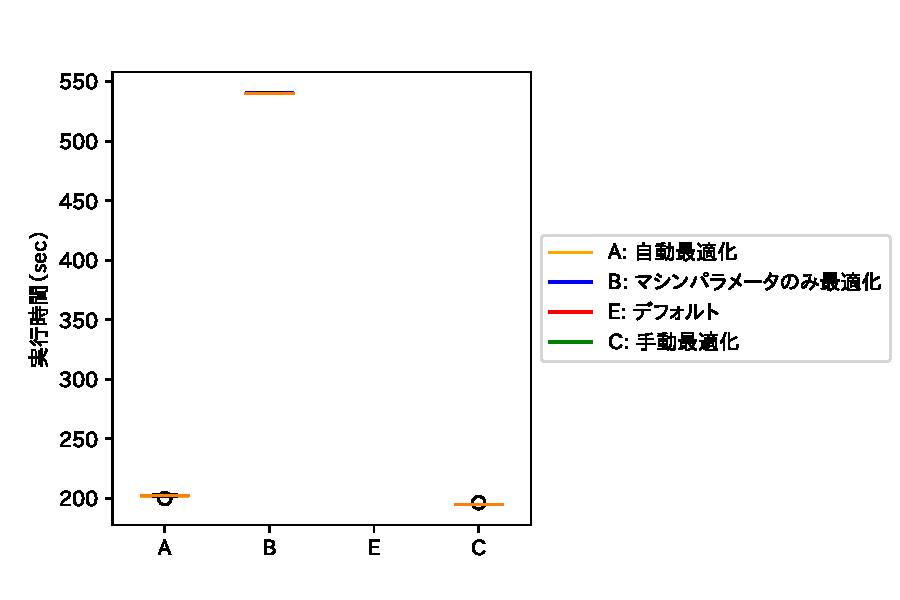
\includegraphics[width=14cm]{./images/k-compare.pdf}
    \caption{京 自動最適化評価}
    \label{fig:k-compare}
  \end{center}
\end{figure}~\\
\begin{figure}[htb]
% h:here, t:top, b:bottom, p:page
 \begin{center}
    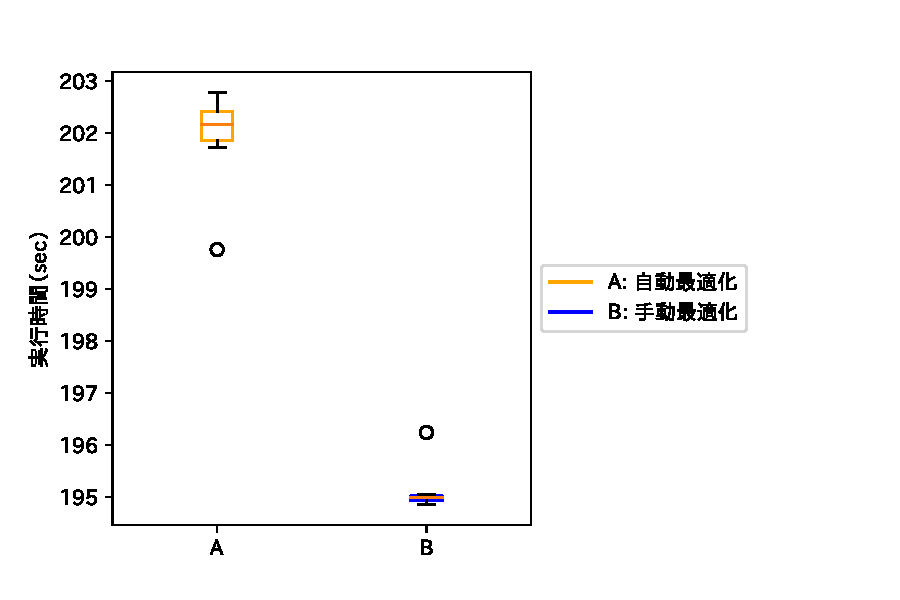
\includegraphics[width=14cm]{./images/k-compare-2.pdf}
    \caption{京 自動最適化評価 (デフォルト以外)}
    \label{fig:k-compare-2}
  \end{center}
\end{figure}~\\
  \clearpage
 最後に自動最適化と手動最適化のみを比較したものを図\ref{fig:k-compare-3}に示す.\\
 先行研究\cite{miyamoto-master}で行われた手動最適化は, この京環境に対して行われていたためクラスタでの実行よりも顕著に差が現れていることが読み取れる. 
この差は, 先行研究\cite{miyamoto-master}においては京上でのみ用いることのできる関数等を用いていることが反映されたものであると考える.\\
\begin{figure}[htb]
% h:here, t:top, b:bottom, p:page
 \begin{center}
    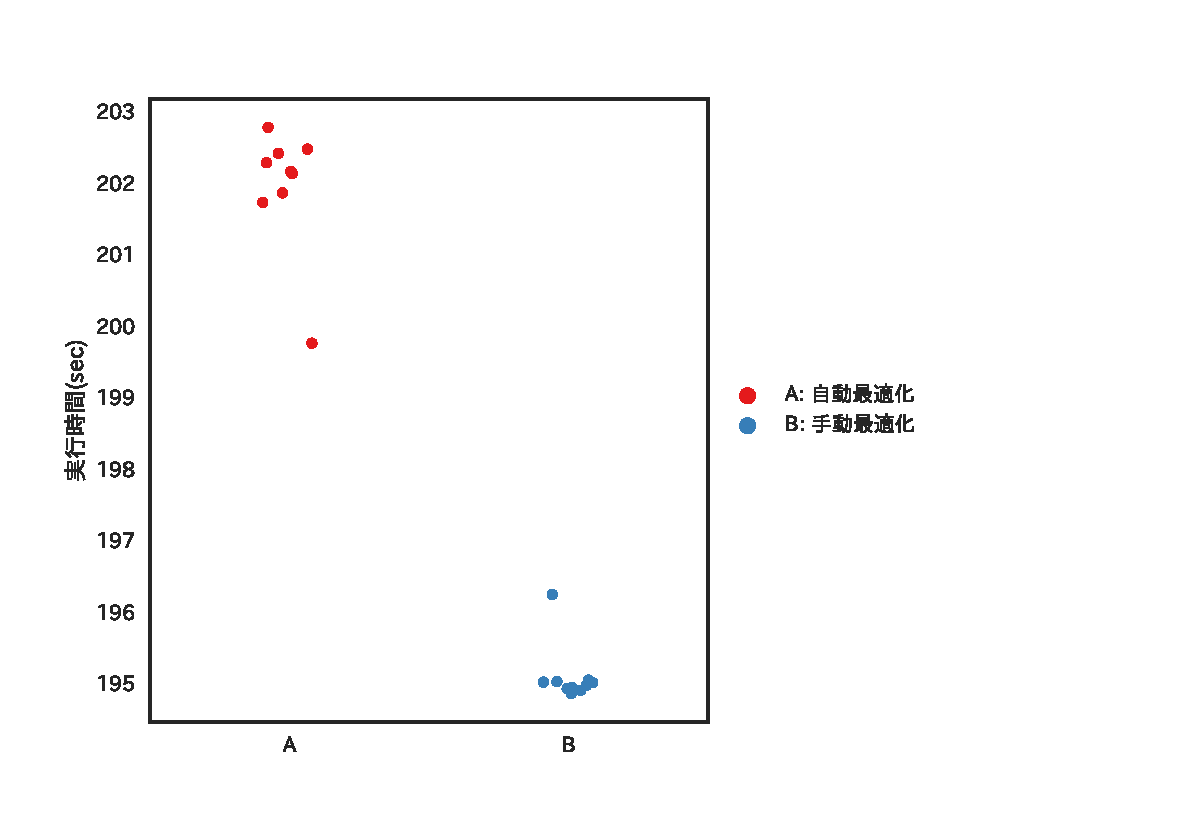
\includegraphics[width=14cm]{./images/k-compare-3.pdf}
    \caption{京 自動最適化評価(自動 vs 手動)}
    \label{fig:k-compare-3}
  \end{center}
\end{figure}~\\
\clearpage
